%------------------------------------------------------------------------------
%
% OS 教科書
%
%------------------------------------------------------------------------------
\documentclass[a4paper,11pt,twocolumn,dvipdfmx]{jsbook}
\usepackage{mySty}
%------------------------------------------------------------------------------
% はじまり
\begin{document}
\frontmatter
%------------------------------------------------------------------------------
% 表紙
\title{オペレーティングシステム\\Ver. 0.0.0}
\author{徳山工業高等専門学校\\情報電子工学科}
\date{}
\maketitle

%------------------------------------------------------------------------------
% 著作権表示
\thispagestyle{empty}
\onecolumn
~
\vfill
\begin{flushleft}
Copyright \copyright ~~ 2017 by \\
Dept. of Computer Science and Electronic Engineering, \\
Tokuyama College of Technology, JAPAN
\end{flushleft}

\vspace{0.8cm}
本ドキュメントはCC-BY-SA 4.0 ライセンスによって許諾されています。

本ドキュメントは
CC-BY-SA 3.0 de ライセンス,
CC-BY-SA 4.0 ライセンス
で許諾された著作物を含みます.

(CC-BY-SA 3.0 de ライセンス全文は
\url{https://creativecommons.org/licenses/by-sa/3.0/de/}で,
CC-BY-SA 4.0 ライセンス全文は
\url{https://creativecommons.org/licenses/by-sa/4.0/deed.ja}で確認できます.)

%------------------------------------------------------------------------------
% 目次
\setcounter{tocdepth}{2}
\tableofcontents

% 本文
%\twocolumn
\mainmatter

% \part{OSの機能を使用してみよう}
% \chapter{システムプログラミング}
% 
\part{OSとは}
\chapter{オペレーティングシステムとは}

オペレーティングシステム(Operating System : OS)は,
Windows,macOS,Linux,FreeBSD,Android,iOS
等である.
皆さんは,これらを使用した経験を持っているだろう.
そして,これらが次のようなソフトウェアから構成されていることを
何となく感じているのではないだろうか.

\begin{enumerate}
\item カーネル(OSの本体)
\item ライブラリ(プログラムが使用するサブルーチン,DLL)
\item ユーザインタフェース(GUI,CLI)
\item ユーティリティソフトウエア
  (ファイル操作,時計,シェル,システム管理 ...)
\item プログラム開発環境
  (エディタ,コンパイラ,アセンブラ,リンカ,インタプリタ)
\end{enumerate}

\emph{広義}では上に列挙した全て\footnote{
  上に挙げたソフトウェアの中で「プログラム開発環境」は,
  LinuxやFreeBSDではOSに含まれているが,
  それ以外では別にインストールする必要がありOSの一部とは言い難くなっている.
}がオペレーティングシステムの一部である.
逆に\emph{狭義}では「カーネル」だけをオペレーティングシステムと考える.
この講義では狭義のオペレーティングシステムの仕組みを勉強する.

%==============================================================================
\section{オペレーティングシステムの役割}
\label{osRole}

オペレーティングシステムの重要な役割は次に述べる二つである.

\subsection{拡張マシンとしてのオペレーティングシステム}
\label{abstruction}

OSはハードウェアの機能を\emph{抽象化}した便利な拡張マシンを提供する.
次に抽象化と拡張マシンの例を示す.

\begin{description}
\item[例1] 二次記憶装置の抽象化(ファイルシステム) \\
  ハードディスク,USBメモリ,CD-ROM等の二次記憶装置は,
  どれもデータを記録する機能を持ったハードウェアである.
  しかし,それらの制御方法や記録されるデータの構造は全く異なる.
  オペレーティングシステムは,
  二次記憶装置をファイルの集合(ファイルシステム)として\emph{抽象化}して
  ユーザプログラム(アプリケーションプログラム)に提供する.

\item[例2] コンピュータそのものの抽象化(プロセス) \\
  プロセスはプロセス専用の仮想CPUと仮想メモリを持つ.
  システムコールを通じて入出力も可能である.
  プロセスはCPU,メモリ,入出力を持っているので
  1台のコンピュータと考えることもできる.

  プロセスはコンピュータを\emph{抽象化}したものだとも言える.
  (プロセス=仮想コンピュータ)

\item[例3] 拡張されたコンピュータ(システムコール) \\
  オペレーティングシステムを備えたコンピュータ上では,
  アプリケーションプログラムがシステムコールを発行できる.
  システムコールを追加命令を考えると,
  オペレーティングシステムを備えたコンピュータは
  追加命令を実行可能な\emph{拡張マシン}だと言える.
  (拡張マシンの命令=機械語命令+システムコール)
\end{description}

オペレーティングシステムが
拡張マシンをアプリケーションプログラムに提供するイメージを
\figref{abstruction}に示す.
ハードウェアの複雑で統一されていない凸凹のインタフェースは,
オペレーティングシステムによってスッキリした円弧の
インタフェース(使いやすい\emph{抽象化}されたインタフェース)に変換される.

オペレーティングシステムの円がハードウェアの外側にあるのは,
オペレーティングシステムによって機能が拡張されたことを示す.
ハードウェアを含む円全体が拡張マシンを表している.

\begin{myfig}{btp}{抽象化}{abstruction}
  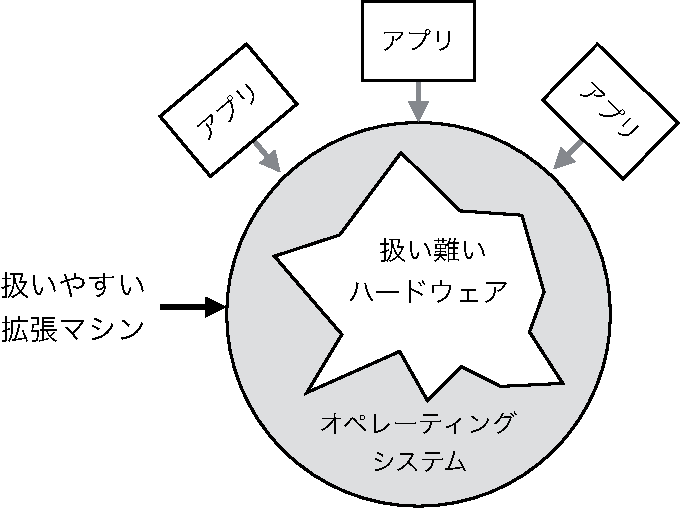
\includegraphics[scale=0.66]{Fig/abstruction-crop.pdf}
\end{myfig}

\subsection{ハードウェア管理プログラムとしてのオペレーティングシステム}
オペレーティングシステムはハードウェア資源を管理・制御し,
アプリケーションプログラムにシステムコール等のサービスを提供する.
\figref{system}はカーネルの役割を説明している.

オペレーティングシステムは,
管理するハードウェア資源をアプリケーションプログラムに割当てる.
複数のアプリケーションプログラムに割り付けるために
資源を\emph{仮想化}して必要な数だけ作り出す.
例えば,CPUは時間を区切って複数のプロセスが共有する
(\emph{時分割多重}による\emph{仮想化}).
メモリはアドレスで区切って複数のプロセスが共有する
(\emph{空間分割多重}による\emph{仮想化}).

\begin{myfig}{btp}{コンピュータシステムの構成}{system}
  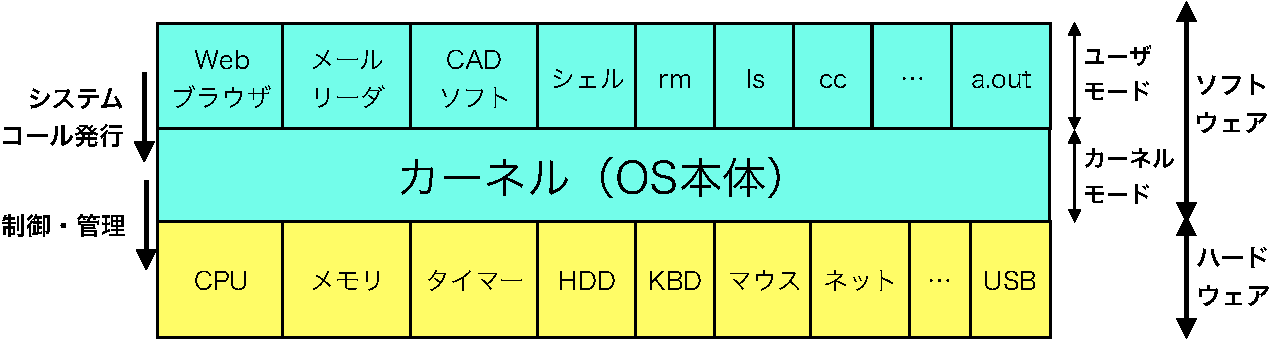
\includegraphics[scale=0.66]{Fig/system-crop.pdf}
\end{myfig}

%==============================================================================
\section{オペレーティングシステムの歴史}

\subsection{第1世代(1945〜1955,真空管の時代)}
初期のコンピュータはコンソールパネルを通して操作する,
巨大なTeC\cite{tec}のようなものだった.
OSは存在せずプログラマはまさにTeCと同様なプログラミングとデバッグを行っていた.

しかし,当時のコンピュータはTeCと異なり大変高価な装置であった.
その高価なコンピュータを一人のプログラマが長時間にわたって
独占使用することになる.
プログラマがバグの原因を考えている間,
とても高価なコンピュータが遊んでしまい勿体ないものであった.

\subsection{第2世代(1955〜1965,トランジスタの時代)}
\label{gen2nd}
コンピュータがトランジスタ回路で製作されるようになり,
\emph{メインフレーム}と呼ばれる大型コンピュータが,
大企業,政府機関や大学等で実用的に使用されるようになった.
メインフレームは数百万ドルと高価だったので,
ハードウェアを遊ばせること無く使用することが優先課題であった.
そこで人手を介すること無く自動的に次々と連続して処理を行う
「コンピュータの自動運転」が行われるようになった.
この処理方式のことは\emph{バッチ処理}と呼ばれた.
\figref{batch}にバッチ処理の概要を示す.

プログラマは\figref{punchcard}のような紙カードに
プログラムやデータを一行ずつ打込む.
100行のプログラムは100枚の紙カードを使用して記録する.
このようにして出来た紙カードの束が一つの処理単位(\emph{ジョブ})になる.
コンピュータでは\emph{バッチモニタ}と呼ばれる常駐プログラムが実行される.
バッチモニタは紙カードからジョブを読み込み実行させる.
ジョブが終了するとバッチモニタに制御が戻り次のジョブが自動的に実行される.
バッチモニタが発展してやがてOSになる.

\begin{myfig}{btp}{バッチ処理}{batch}
  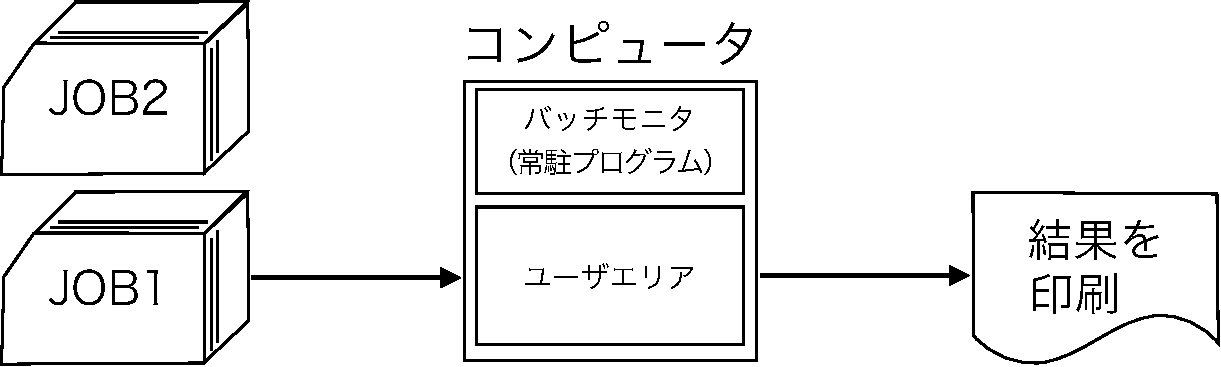
\includegraphics[scale=0.5]{Fig/batch-crop.pdf}
\end{myfig}

\begin{myfig}{btp}{紙カード}{punchcard}
  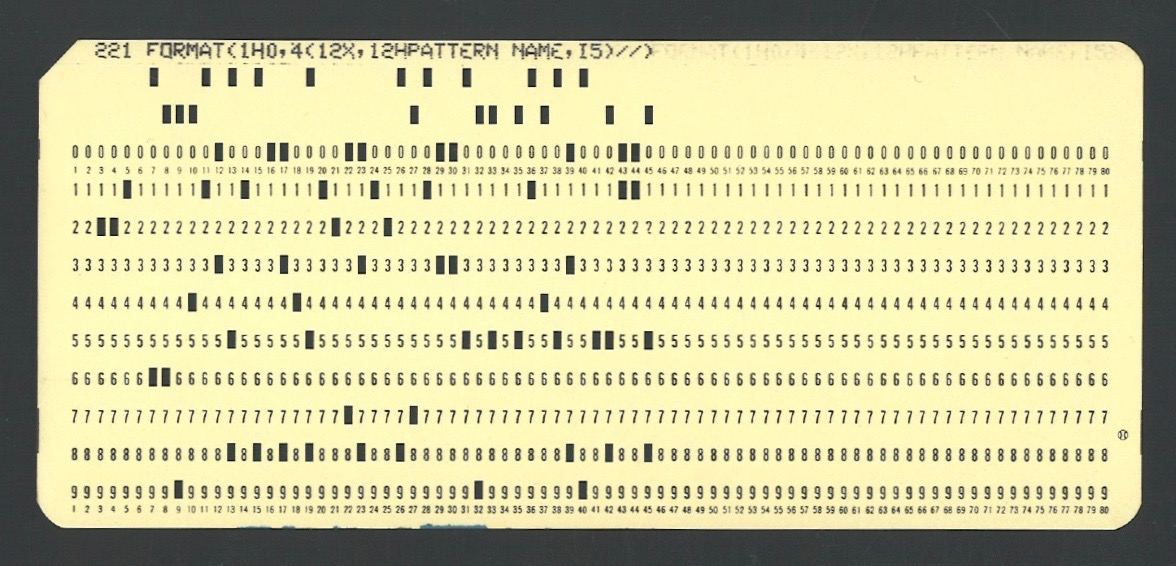
\includegraphics[scale=0.3]{Photo/punchcard.jpg}
\end{myfig}

この方式でうまく処理できるように,次のような発明があった.

\begin{enumerate}
\item \emph{JOB制御言語(JCL : Job Control Language)} \\
  バッチモニタを制御するコマンド言語をJOB制御言語(JCL)と呼ぶ.
  JCLコマンドはジョブ途中の紙カードに記載する.
  \figref{job}にJCLを含むジョブの構成を示す.
  これは,
  FORTRAN言語で記述したプログラムを実行し,
  後半にあるデータを処理するジョブの例になっている.

  \begin{myfig}{btp}{ジョブの構成}{job}
    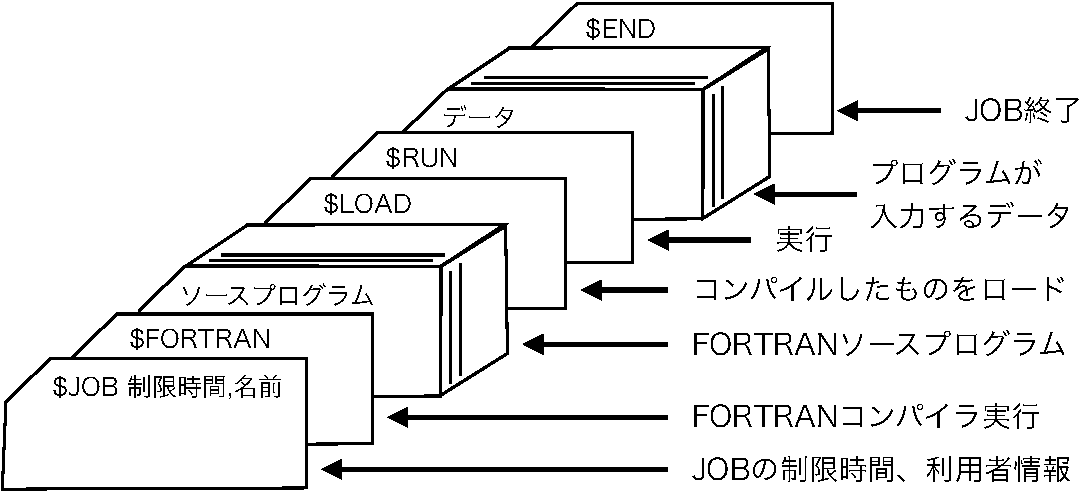
\includegraphics[scale=0.5]{Fig/job-crop.pdf}
  \end{myfig}

\item \emph{実行モード} \\
  ユーザプログラム(ジョブ)のバグで
  バッチモニタが破壊されないようにするために,
  ユーザプログラム実行中なのかバッチモニタ実行中なのか区別する必要がある.
  どちらを実行中なのかを示すハードウェアのフラグを導入し,
  \emph{ユーザモード}と
  \emph{カールモード}(\emph{スーパバイザモード}とも呼ぶ)を
  区別するようになった.
  ユーザモードではハードウェアへのアクセスや,
  実行できる機械語命令に制限がある.

\item \emph{システムコール} \\
  ユーザプログラムが直接に入出力装置等にアクセスすることは,
  バッチ処理を継続できなくする恐れがあるので許されない.
  例えばユーザプログラムがハードウェアのモードを切り換えてしまうと,
  以降のジョブが正常に実行されなくなる恐れがある.
  そこで,ユーザプログラムはバッチモニタに依頼(システムコール)して
  入出力を行う必要がある.

  プログラムが終了する時は
  カーネルモードに切り換えてバッチモニタに戻る必要がある.
  カーネルモードに切り替える機械語命令をユーザプログラムが実行可能だと,
  実行モードが無意味になるので許可すべきではない.
  システムコールを使用してプログラムを終了する.

\item \emph{記憶保護} \\
  ユーザプログラムのバグでバッチモニタが破壊されないように,
  ユーザモードで実行中は
  主記憶のバッチモニタ領域に書込みができないようにする.
\end{enumerate}

\subsection{第3世代(1966〜1980,ICとマルチプログラミングの時代)}
1960年代のコンピュータはIC(Integrated Circuit)を用いて作られるようになり
価格性能比が随分改善された.
第3世代と呼ばれる当時のオペレーティングシステムの中には,
現代のオペレーティングシステムの先祖であったり,
強い影響を与えたものがある.
\figref{tree}に第3世代から現代に至るまでの系統図を示す.


IBMが開発したSystem/360(\figref{system360})は高価な大型のものから,
安価な小型のものまでで同じオペレーティングシステムが使用でき,
同じユーザプログラムを実行できる\emph{シリーズ化}を行い商業的に大成功をおさめた
\cite{third}.
System/360はそれ以前のものとは異なり科学技術計算にも事務処理にも使用できる.
System/360のオペレーティングシステムは,
1966年にデビューしたOS/360である.
\figref{tree}に示すように,
OS/360の子孫であるz/OSが現代でも使用されている\cite{os360}.

\begin{myfig}{btp}{フォルクスワーゲンで使われているSystem/360}{system360}
  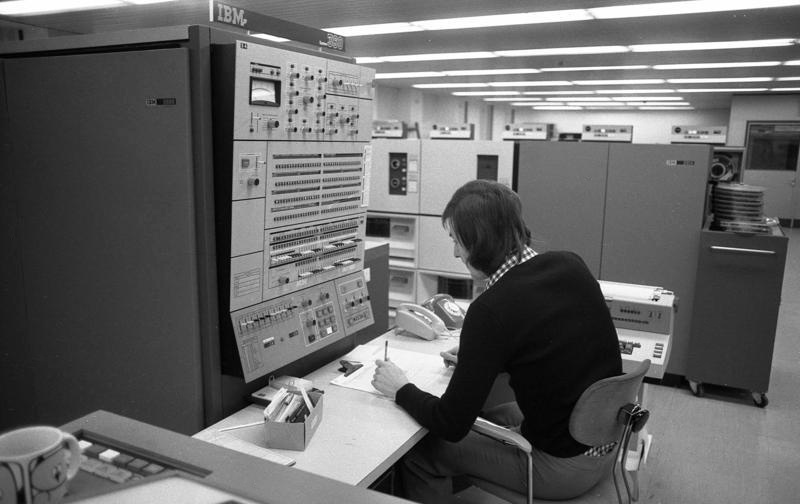
\includegraphics[scale=0.25]
  {Photo/Bundesarchiv_B_145_Bild-F038812-0014,_Wolfsburg,_VW_Autowerk.jpg}\\
  {\small
    ウィキメディア /
    Bundesarchiv, B 145 Bild-F038812-0014 /
    Schaack, Lothar / CC-BY-SA 3.0 de}
\end{myfig}

OS/360を含む第3世代のオペレーティングシステムが
実現した重要な新しい機能を紹介する.

\begin{itemize}
\item \emph{仮想記憶} \\
  主記憶を仮想化し実際より大きい主記憶があるように見せる.
  実際の主記憶より大きいプログラムが実行可能になる.

\item \emph{マルチプログラミング} \\
  \label{multiprogramming}
  \figref{multiprogramming}のように,
  複数のプログラム(ジョブ)を主記憶にロードしておき,
  その中で実行可能なものを選んで実行する.
  入出力待ち等で実行できなくなったら他のプログラムを実行する.
  高価なCPUが入出力待ちで停止する可能性を低くすることができた.

  \begin{myfig}{btp}{マルチプログラミングシステム}{multiprogramming}
    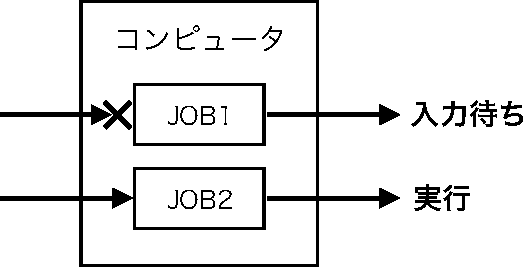
\includegraphics[scale=0.66]{Fig/multiprogramming-crop.pdf}
  \end{myfig}

\item \emph{タイムシェアリング(TSS:Time Sharing System)} \\
  マルチプログラミングの一種である.
  \figref{timesharing}のように,
  複数のターミナルをコンピュータに接続し
  複数のユーザが同時にコンピュータを使用できるようにする.
  短時間(例えば10ms)で処理するジョブを次々に切り換えることで,
  ユーザは自分がコンピュータを独占しているように感じることができる.
  なお,ターミナルは\figref{terminal}のような,
  キーボードと表示装置だけを備えた安価な装置である.

  \begin{myfig}{btp}{タイムシェアリングシステム}{timesharing}
    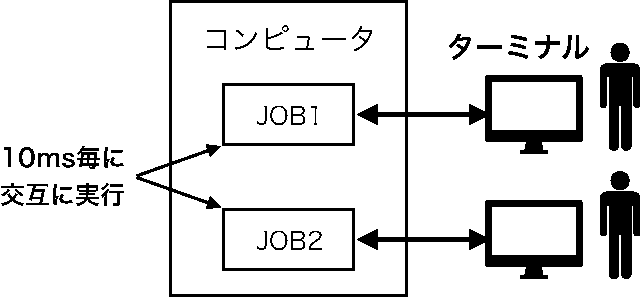
\includegraphics[scale=0.66]{Fig/timesharing-crop.pdf}
  \end{myfig}

  \begin{myfig}{btp}{ターミナル}{terminal}
    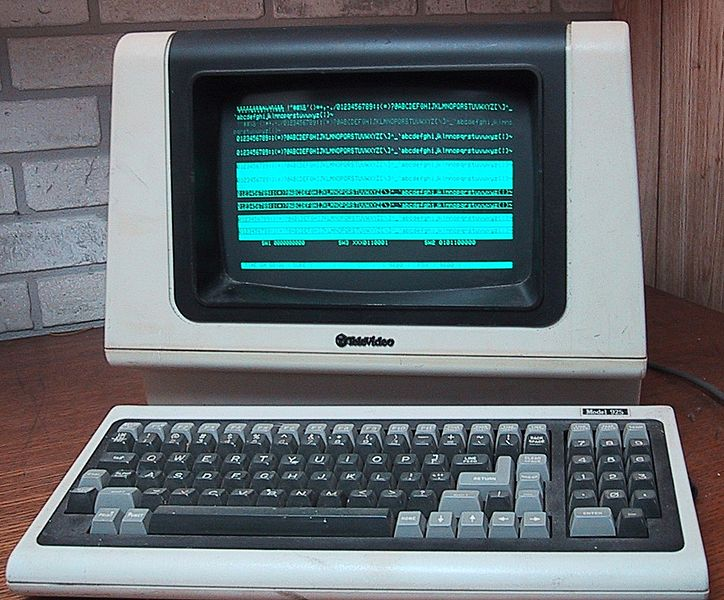
\includegraphics[scale=0.25]
     {Photo/724px-Televideo925Terminal.jpeg}\\
     {\small 写真:
       \url{http://commons.wikimedia.org/wiki/File:Televideo925Terminal.jpg}
       (パブリックドメイン)}
  \end{myfig}
\end{itemize}

この時代のオペレーティングシステムやコンピュータシステム,
そして,それらの開発プロジェクトの中で,
その後のオペレーティングシステムに多くの影響を与えた有名なものを紹介する.

\begin{itemize}
\item OS/360 \\
  世界初の本格的な商用オペレーティングシステムである.
  メインフレームの主流OSとなり子孫は現在でも使用されている\cite{os360}.

\item MULTICS(MULTiplexed Information and Computing Service)プロジェクト
  \cite{third} \\
  MIT,ベル研究所,General Electricが共同で始めた
  巨大で強力なコンピュータシステムを構築するプロジェクトである.
  強力な一台のコンピュータで
  都市一つ分のコンピュータサービスを提供する構想だった.
  完成までに長い期間を要し(その間にベルとGEが脱落し),
  商業的には失敗であったがその後のオペレーティングシステムに影響を与える
  多くのアイデアが出てきた.

\item UNIX(ユニックス) \\
  MULTICSプロジェクトから抜けたベル研のKen Thompsonらにより開発された
  \cite{unix}.
  \figref{tree}に示すように,
  現代のオペレーティングシステムの多くがUNIXを起源にしている.
  子孫ではないものもUNIXの影響を強く受けている.
  LinuxはUNIX互換のオペレーティングシステムを作ろうとして
  開発が始まった\cite{linux}.
  Androidの中身はLinuxである\cite{android}.
  z/OSはUNIX互換環境を備えている\cite{zos}.
  WindowsにもUNIX互換環境(POSIXサブシステム)を
  利用可能なものがある\cite{windows}.

\item DynaBook(ダイナブック:OSだけでなくコンピュータ全体を指す)
  \cite{dynabook2} \\
  アラン・ケイが1972年に著した
  「A Personal Computer for Children of All Ages」\cite{key72, key72J}
  に登場する理想のパーソナルコンピュータである.
  アラン・ケイがゼロックスのパロアルト研究所に在籍中の1970年代に開発した
  Alto上の「暫定ダイナブック環境」(\figref{smalltalk})は
  既にGUIやマウスを使用していた.
  スティーブ・ジョブスがAltoを見たことが
  LISA開発きっかけになったと言われている\cite{dynabook}.

  \begin{myfig}{btp}
    {Alto(Alto エミュレータ)のスクリーンショット}
    {smalltalk}
    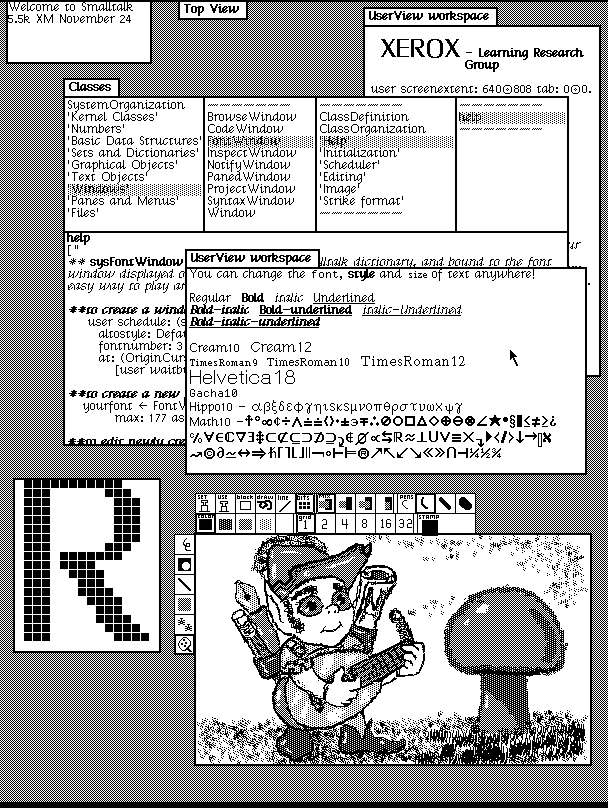
\includegraphics[scale=0.5]{Photo/Smalltalk-76.png}\\
                    {\small
                      ウィキメディア /
                      SUMIM.ST /\\
                      AltoやNoteTakerで動作した
                      アラン・ケイ達の暫定Dynabook環境
                      (Smalltalk-76、同-78の頃) /
                      CC-BY-SA 4.0
                    }
  \end{myfig}

\end{itemize}

\subsection{第4世代(1980〜現代,PCの時代)}

1970年代に単一のLSIにCPU全体を集積したマイクロプロセッサが登場した.
1970年代中頃にはマイクロプロセッサを用いて個人向けのコンピュータである
パーソナルコンピュータ(当時はマイクロコンピュータと呼んでいた)
を作ることが可能になった.
それに伴いパーソナルコンピュータ用のオペレーティングシステムが登場した.

\begin{enumerate}
\item 8bitマイクロコンピュータの時代 \\
  1977年にDigtal Reserch社がCP/M(Control Program for Microcomputer)と呼ばれる
    8bitマイクロコンピュータ用の簡単なオペレーティングシステムを
    開発し成功した.
    しかしこのオペレーティングは16bitパーソナルコンピュータの時代には
    早々に消え去ってしまった\cite{fourth}.

  \item 16bitパーソナルコンピュータの時代 \\
    IBMが1981年に16bitパーソナルコンピュータIBM PC\cite{ibmpc81}
    (\figref{ibmpc})を発売した.
    IBM PCは現在のWindows PCの先祖である.
    IBM PCの子孫は改良や拡張を続けながら現在まで高いシェアを維持し続けている.
    IBM PCのオペレーティングシステムとして開発されたのが,
    Microsoft社のMS-DOS(MicroSoft Disk Operating System)\cite{msdos}である.
    バージョン2からはUNIXのような
    階層ディレクトリやパイプ,リダイレクト等の機能を持っている.
    \figref{tree}に示すように,MS-DOSはWindowsに置き換わりWindows MEまで
    バージョンアップが繰り返された.

    \begin{myfig}{btp}{IBM PC}{ibmpc}
      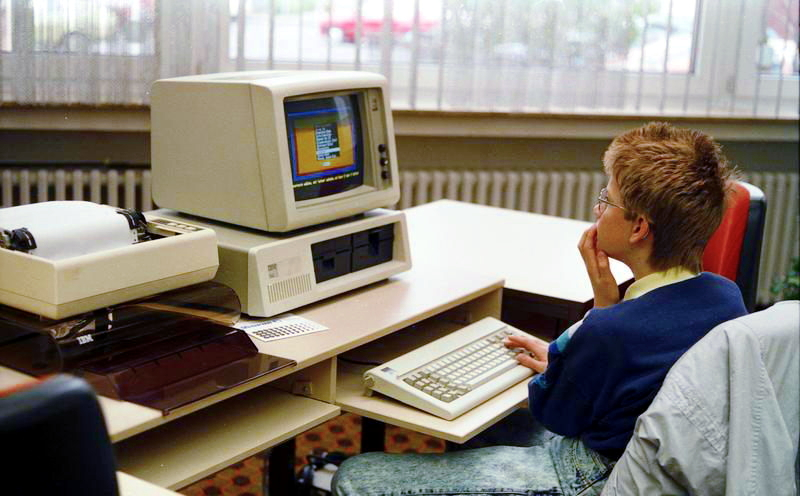
\includegraphics[scale=0.35]
                      {Photo/Bundesarchiv_B_145_Bild-F077948-0006,_Jugend-Computerschule_mit_IBM-PC.jpg}\\
                      {\small
                        ウィキメディア /
                        Bundesarchiv, B 145 Bild-F077948-0006 /
                        Engelbert Reineke / CC-BY-SA 3.0 de}
    \end{myfig}

    Apple社は1984年にMacintosh(\figref{macintosh})を発売した.
    MachintoshのOSであるMacOSはLISAを経てDynaBook\cite{key72, key72J}の
    影響を受けていると言われている\cite{fourth}.
    \figref{tree}に示すように,
    当初のMacOSはMacOS 9\cite{classicmacos}まで改良が続けられた.

    \begin{myfig}{btp}{初代Macintosh}{macintosh}
      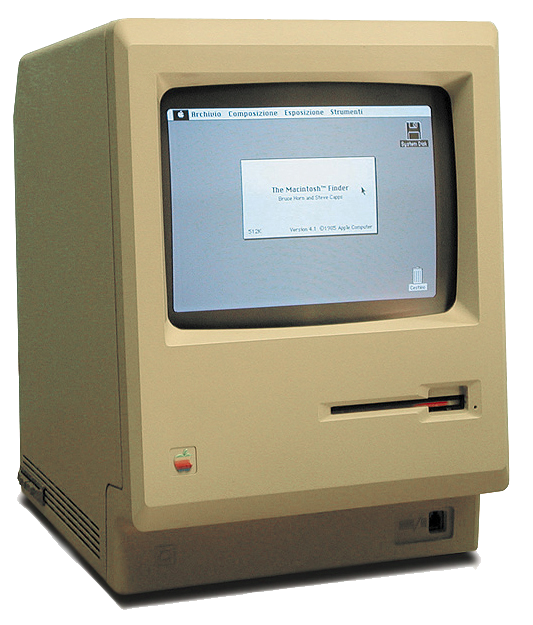
\includegraphics[scale=0.25]{Photo/Macintosh_128k_transparency.png}\\
                      {\small
                        ウィキメディア / w:User:Grm wnr /
                        File:Macintosh 128k transparency.png /GFDL}
    \end{myfig}

  \item 32bitパーソナルコンピュータの時代 \\
    1990年頃には32bitのマイクロプロセッサが
    パーソナルコンピュータにも使用されるようになった.
    32bitのマイクロプロセッサは実行モードを備え,
    またメモリ管理ユニットも利用可能であった.
    つまり,カーネルモードとユーザモードを使い分けたり
    仮想記憶を利用する本格的な第3世代のオペレーティングシステムを
    実行できる環境がパーソナルコンピュータにも整った.

    そこで,
    従来ワークステーションやミニコンで使用されていた
    UNIXを安価なパーソナルコンピュータ(特にIBM PC互換機)で
    動くようにする人たちが現れ,
    オープンソースソフトウェアとしてLinuxやFreeBSD等の開発が始まった.
    また,もともとパーソナルコンピュータ用のWindowsやMacOSも
    32bitマイクロプロセッサの機能を使いこなす
    本格的なオペレーティングシステムに生まれ変わった.

    \begin{itemize}
    \item Linux \\
      1991年に開発が始まったLinuxはUNIX互換のオペレーティングシステムを
      パーソナルコンピュータ(IBM PC互換機)用に
      独自に作成したものである\cite{linux}.
      Linuxは改良され続け,
      現在ではパーソナルコンピュータだけでなく,
      スーパーコンピュータ「京」のオペレーティングシステム\cite{kei}から,
      スマートフォンのオペレーティングシステムであるAndroid\cite{android},
      テレビ等の組込みシステムのオペレーティングシステムまで,
      広く使われるようになっている.

    \item BSD 系の UNIX \\
      386BSD\cite{386bsd}はBSD UNIXをIntel 80386 CPUを搭載した
      パーソナルコンピュータ(IBM PC互換機)で動作するようにしたものである.
      386BSDはFreeBSD等に受継がれるがUNIXのライセンス問題が発生する\cite{unix}.
      ライセンス問題が片付き安心して使用できるようになった
      4.4BSD-Lite Release 2\cite{unix}をベースに
      FreeBSD, NetBSD, OpenBSD 等の多くの BSD 系 PC-UNIXが開発された.

      その後,FreeBSDは MacOS X に取り込まれている.
      また,FreeBSDにZFSが移植された\cite{zfs}ので
      ファイルサーバ用に特化したFreeNAS\cite{freenas}にも使用されている.
      なお,徳山工業高等専門学校・情報電子工学科のパソコン室では
      1993年10月に386BSDの利用を開始して以来,
      2014年3月までFreeBSDを学生用PCやサーバのオペレーティングシステムとして
      使用してきた\cite{iebsd}.

    \item System V 系の UNIX \\
      System V の流れを汲むSolaris\cite{solaris}は,
      RISC マイクロプロセッサ SPARC を搭載するサーバやワークステーションでも,
      パーソナルコンピュータ(IBM PC 互換)でも使用できる.

    \item 従来のパーソナルコンピュータ用オペレーティングシステム \\
      従来のWindowsやMacOSはCPUの実行モード等を使用していなかったので,
      アプリケーションプログラムのバグにより
      システム全体が停止するようなトラブルを防ぐことができなかった.
      そこで,32bitマイクロプロセッサの使用を前提に新しく作り直された.

      新しく作り直された32bitのWindows NT系列の製品は,
      徐々に従来のWindowsを置換えた.
      (\figref{tree}参照).
      現在(2017年10月)の最新版はWindows 10である.

      MacOS は,2001年にUNIXの流れを汲み安定して動作するOPENSTEPベースの
      MacOS X\cite{macos}に置き換わった(\figref{tree}参照).
      その後,名称が OS X, macOS と変更されたがこれらは MacOS X の改良版である.
      現在(2017年10月)の最新版はmacOS 10.13 High Sierraである.
      iPhoneのiOSはMacOS Xをタッチパネル用に再構成したものである\cite{ios}.
    \end{itemize}
\end{enumerate}

\subsection{インターネット世代}
現在のオペレーティングシステムはTCP/IP機構が組込まれ
インターネットに接続することができる.
今ではパーソナルコンピュータやスマートフォンの使用を
インターネット抜きに考えることができない.
オペレーティングシステムにとってインターネットに接続できることは
重要なことである.

TCP/IPを実装した4.2BSDが1984年に公開された\cite{bsd}.
以来,4.2BSDの子孫はインターネットに対応している.
1988年に公開されたSystem V R4はBSD起原のTCP/IPの実装を含んでいた\cite{svr4}.
これの子孫もインターネットに対応している.
Linuxも1.0の頃にはTCP/IPの実装を含んでいた\cite{linux1}.
WindowsはWindows 95からTCP/IPを標準装備している\cite{windows}.
MacOSはMacOS 8が発表されるまでにはインターネット対応がされていた
\cite{classicmacos}.
メインフレームの世界でもOS/390はインターネットに対応した\cite{os390}.

このようにして1990年代の後半には多くのオペレーティングシステムが
インターネット対応を完了させた.
インターネット対応を完了させたオペレーティングシステムを
「インターネット世代のオペレーティングシステム」と言うことができる.

\begin{myfig}{btp}{オペレーティングシステムの系統図}{tree}
  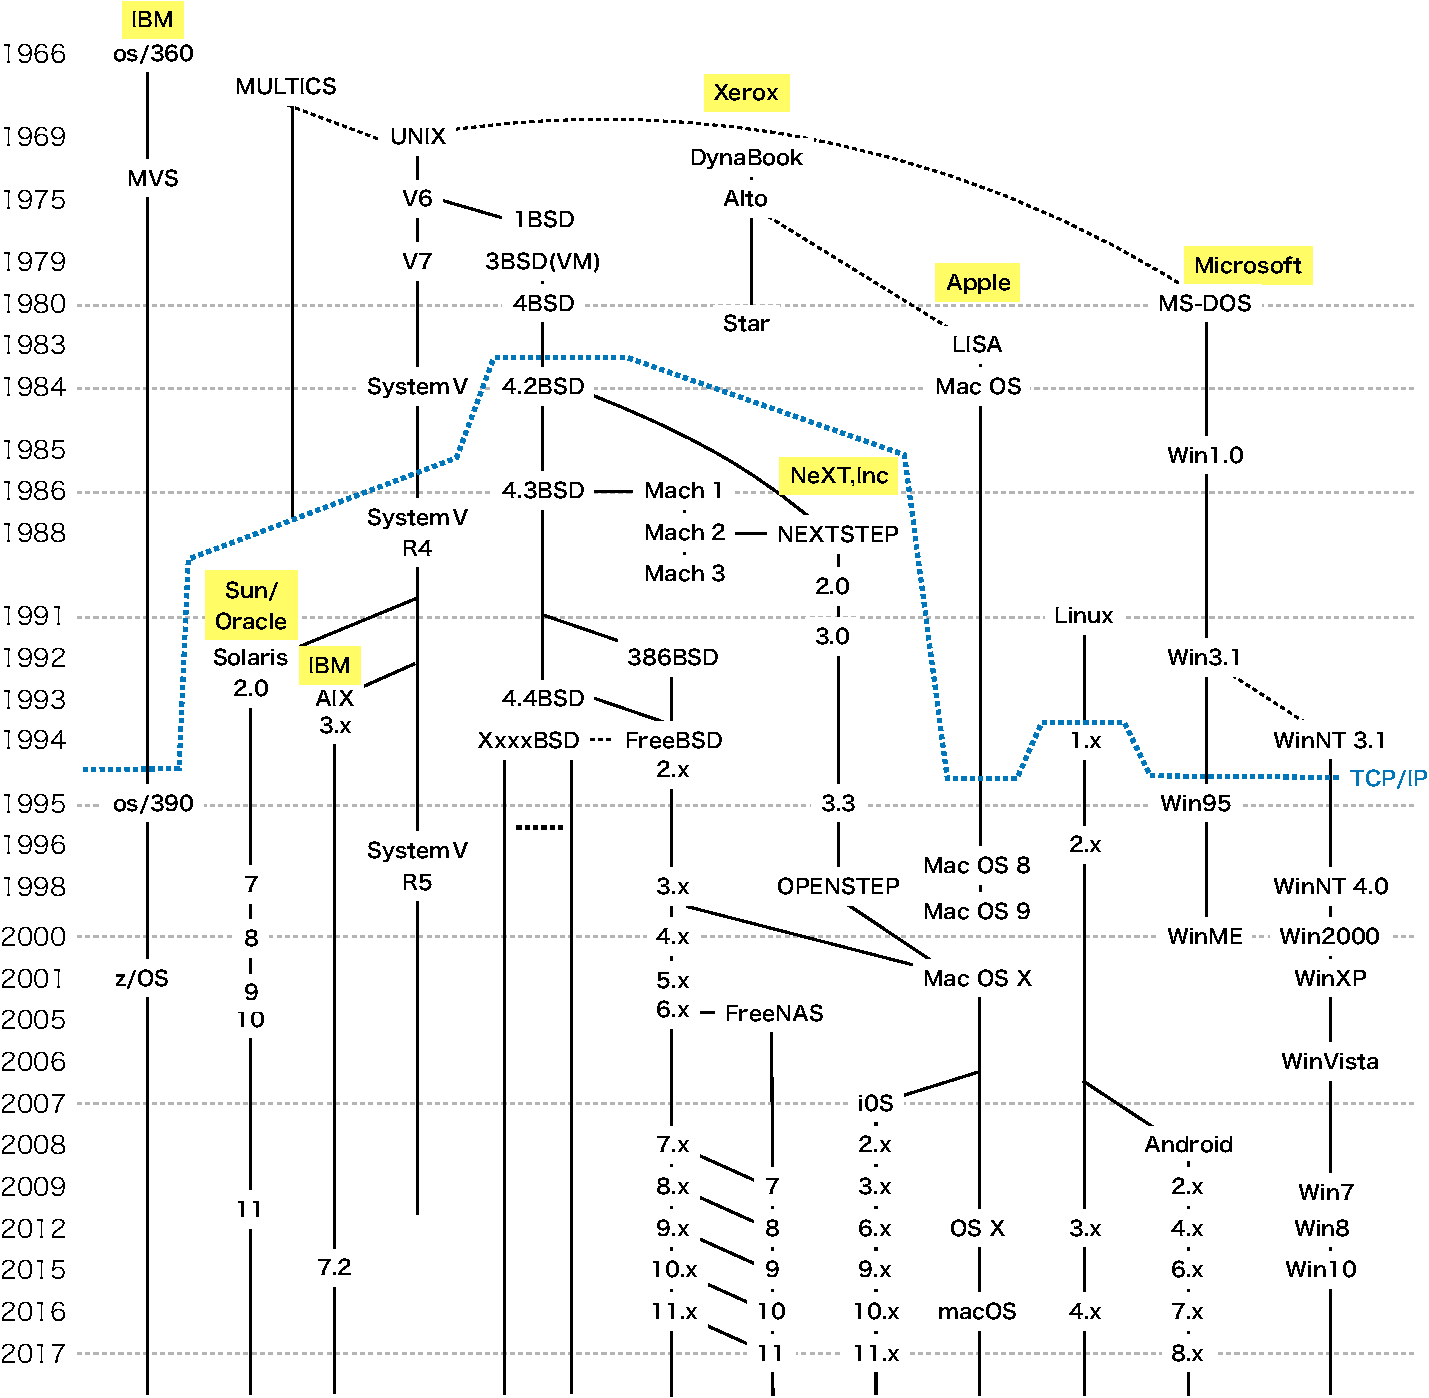
\includegraphics[scale=0.6]{Fig/tree-crop.pdf}\\
                  {\small
                    系統図は\cite{os360,
                      mvs,
                      os390,
                      zos,
                      unix,
                      solaris,
                      aix,
                      mach,
                      bsd,
                      bsdd,
                      386bsd,
                      freebsd,
                      freenas,
                      nextstep,
                      classicmacos,
                      dynabook,
                      macos,
                      ios,
                      linux,
                      android,
                      msdos,
                      windows}
                    の内容を総合して作成した.}
\end{myfig}

%==============================================================================
\section{まとめ}
狭義のオペレーティングシステムは\emph{カーネル}のことを指す.
本書は狭義のオペレーティングシステムについて述べている.

オペレーティングシステムの重要な役割りは,
コンピュータの資源を\emph{抽象化}することと\emph{仮想化}することである.
オペレーティングのユーザは,
使いやすい抽象化されたインタフェースを通して資源を利用できる.
また,ユーサは仮想化された資源を必要なだけ独占して使用することができる.

オペレーティングシステムは,
1950年代に出現したバッチモニタから進化してきた.
現在では,
スーパーコンピュータから組み込み用コンピュータまで,
非常に広い範囲のコンピュータが本格的なオペレーティングシステムを搭載している.


%==============================================================================
\section*{練習問題}
\begin{enumerate}
  \renewcommand{\labelenumi}{\ttfamily\arabic{chapter}.\arabic{enumi}}
  \setlength{\leftskip}{1em}
\item \emph{抽象化}について説明しなさい.
\item \emph{抽象化}の例をいくつか挙げなさい.
\item \emph{仮想化}について説明しなさい.
\item \emph{仮想化}の例をいくつか挙げなさい.
\item 自分がいつも使用しているコンピュータやスマートフォンの
  オペレーティングシステムの種類を調べなさい.
\end{enumerate}
 % オペレーティングシステムとは
\chapter{前提知識}
以下では,
本書で想定しているコンピュータのハードウェアやソフトウェアの
構成について解説する.

\section{コンピュータのハードウェア構成}
本書は,
コンピュータのハードウェア構成が\figref{hardBlock}のようになっている
ことを前提にしている.
複数のCPU(Central Processing Unit)がメモリを共有し,
また,全てのCPUは同じ機能を持ち優劣が無い.
このような方式を
{\bf SMP(対称型マルチプロセッシング:Symmetric Multiprocessing)}と呼ぶ.
メモリはCPUだけでなく,
I/Oコントローラ(\figref{hardBlock}ではアダプタやコントローラ)にも
共有される.

\myfigure{btp}{scale=0.48}{Fig/hardBlock-crop.pdf}{ハードウエア構成}{hardBlock}

\begin{enumerate}
\item CPU \\
CPUはコンピュータの頭脳である.
図はCPUが二つの構成になっているが,
実際は一つの場合も,もっと多い場合もある.

\item メモリ(主記憶装置) \\
プログラムやデータを記憶し,
プログラム実行する際にCPUが直接使用する記憶装置である.

\item タイマー \\
一定間隔で繰り返しCPUに割り込みを発生するインターバルタイマーである.

\item グラフィックアダプタ \\
ディスプレイを接続するためのアダプタである.
表示内容を記憶するメモリを独自に持つ場合と,
主記憶装置を使用する場合がある.
最近のパーソナルコンピュータでは,
グラフィックアダプタにGPU(Graphics Processing Unit)が組込まれている.

\item SATA ホストコントローラ \\
SATA(Serial Advanced Technology Attachment)は,
パーソナルコンピュータと二次記憶装置(ハードディスクやCD-ROM)を接続するための
インタフェース規格である.
SATA ホストコントローラは次のような動作をする.
\begin{enumerate}
\item CPUがSATAホストコントローラにコマンドを書き込む.
コマンドは,
「読み/書き」,「セクタアドレス」,「セクタ数」,「メモリアドレス」
を含んだものである.
\item SATAホストコントローラは,
ディスクコントローラと通信しハードディスクにコマンドを渡す.
\item ハードディスクの読み・書きが可能になったら,
ホストコントローラはハードディスクとメモリの間でデータ転送を行う.
このようなCPUを介さないデータ転送のことを,
{\bf DMA(Direct Memory Access)}と呼ぶ.
\item SATAホストコントローラはCPUに割り込み信号を送り,
データの転送が完了したことを知らせる.({\bf I/O完了割り込み})
\end{enumerate}
CPUは,
SATAホストコントローラにコマンドを送ってから割り込みが発生するまでの間,
他の仕事をすることができる.
ハードディスクの操作(I/O操作)とCPUの計算は並列実行される.

\item USBコントローラ \\
USB(Universal Serial Bus)は,
パーソナルコンピュータと周辺装置を手軽に接続できるインタフェースである.
USBメモリスティックやプリンタ,キーボード,マウス等,多くの周辺装置が
USBを通して接続できる.
USBコントローラもSATAホストコントローラのようにDMA機能を備えている.

\item ネットワークアダプタ \\
パーソナルコンピュータのネットワークアダプタは,
GbE(Gigabit Ethernet)規格のものが普及している.
これもSATAホストコントローラのようにDMA機能を備えている.

\item BUS(バス) \\
パーソナルコンピュータのハードウェアを構成する装置の間で
データをやり取りするための配線である.
CPUだけでなくDMAを使用するコントローラやアダプタが大量のデータ転送を行うので,
バスのデータ転送能力がパーソナルコンピュータの性能向上のボトルネックになる.

そのため後で説明するように,実際の物理的な接続は\figref{hardBlock}とは
かなり異なった構成になっている.
しかし,オペレーティングシステムが意識しなければならない論理的な
接続は\figref{hardBlock}のようなものである.

\end{enumerate}

\section{CPUの構成}
本書では、CPUは\figref{cpuBlock}のような部品で構成されると考える.
\figref{hardBlock}に示したように,CPUはBUSを通して他の装置と接続される.
CPUは,一つの機械語命令の実行が終わり次の命令の実行を開始する前に,
他の装置から割り込みを受け付けることができる\footnote{
例外的に,メモリ管理に関する一部の割込は機械語命令の途中で発生する.}.

\myfigure{btp}{scale=0.66}{Fig/cpuBlock-crop.pdf}{CPUの構成}{cpuBlock}

\begin{enumerate}
\item {\bf PSW(Program Status Word)} \\
PSWは,PC(Program Counter)とFlags(フラグ)から構成されるものとする
\footnote{
教科書によっては,フラグだけをPSWと呼ぶ場合もある.}.
PCはCPUが実行中のプログラムの命令アドレスを保持するカウンタである.
Flagsは計算の結果によって変化するフラグの他に,
割り込み許可/不許可を表現するビット,
実行モード(ユーザモード/カーネルモード)を表現するビット等が含まれる.

\item {\bf CPUレジスタ} \\
計算に使用するCPUの汎用レジスタのことである.
TeCではG0,G1,G2,SPのこと,
情報処理技術者試験のCOMETではGR0,GR1,GR2,GR3,GR4のことである.

\end{enumerate}

PSWとCPUレジスタは,
機械語命令を実行する毎に値が変化・確定しプログラムが意識している\footnote{
一方でCPU内部にはプログラムから見えないレジスタもある.
}ので,CPUを仮想化し実行するプロセスを切換える際に保存・復旧の対象となる.

\section{最近のコンピュータの実際の構成}

Intel社のCPUを使用したデスクトップ・パーソナルコンピュータと
サーバコンピュータの構成を説明する.
バスがボトルネックにならないように,
CPUにメモリを直接接続してある.

\subsection{デスクトップ・パーソナルコンピュータ}
\figref{intelDesktop}はIntel社のCPUを使用した
近年のデスクトップ・パーソナルコンピュータの構成を表している.
Intel社の用語では,これまで「CPU」と読んでいたものが
「{\bf Core(コア)}」と呼ばれる.
「CPU」は複数のコアを含んだLSIのことを指している.
デスクトップ用のCPUには1〜4個のコアが集積されている.

コアに隣接しているL1はレベル1キャッシュ(Level 1 cache)を表している.
L2は複数のコアにシェアされるレベル2キャッシュ(Level 2 cache)を表している.
メモリとのデータ転送量が多いCoreとGPUがCPUに集積され,
I/O装置のコントローラやアダプタはPCHに集積されている.
CPUとPCHはDMIと呼ばれる専用のインタフェースを用いて接続される.

\myfigure{btp}{scale=0.66}{Fig/intelDesktop-crop.pdf}
{デスクトップPCの構成}{intelDesktop}

\subsection{サーバコンピュータ}
より強力な処理能力が必要なサーバ用コンピュータでは,
\figref{intelServer}のように多くのコアを内蔵するCPUを複数個使用する.
現在(2017年秋)最新の Intel Xeon Processor Scalable Family の場合,
CPU同士はUPIと呼ばれる高速な専用インタフェースで接続される.
最大の構成は,28コアのCPUを8個使用し合計224コアのものである.
PCHもサーバ用のものでは,より多くのストレージやネットワークを接続できる.

\myfigure{btp}{scale=0.5}{Fig/intelServer-crop.pdf}
{サーバPCの構成}{intelServer}

\section{オペレーティングシステムの構造}
\figref{osOrganization}にオペレーティングシステムの構造を示す.
オペレーティングシステムのカーネルは
\figref{osOrganization}中央部分のソフトウェアである.
ユーザプロセスはユーザモードで,
カーネルはカーネルモードで実行される.

\subsection{カーネルの構成}
\figref{osOrganization}に示すように,
カーネルは以下のようなモジュールから構成される.

\begin{enumerate}
\item {\bf 割り込みハンドラ} \\
割込みが発生した時に自動的に実行される割込み処理ルーチンである.
割込みが発生した原因を判断し,必要なモジュールを呼出す.
例えば,タイマーからの割込みならタイマーのデバイスドライバを呼出す.

\item {\bf ディスパッチャ} \\
カーネルの処理が終了した時,
実行可能なプロセスの中から一つを選んで実行を再開させる.

\item {\bf コア} \\
割込みハンドラとディスパッチャを含むコアは,
資源の仮想化を行うために必ずカーネルモードで実行される必要がある部分である.

\item {\bf サービスモジュール} \\
サービスモジュールは,
ハードウェアを抽象化した便利なコンピュータを
ユーザ・プロセスに提供するためのプログラムである.
\end{enumerate}

\myfigure{btp}{scale=0.66}{Fig/osOrganization-crop.pdf}
{オペレーティングシステムの構造}{osOrganization}

\subsection{カーネルの動作概要}
通常,コンピュータはユーザ・プロセスを実行し目的の仕事をしている.
何かイベントが発生すると割込みによりCPUに通知される.
CPUはカーネルモードに切り替わり割込みハンドラに制御を移す.
CPUがユーザ・プロセスの実行からカーネルの実行に移行するのは,
{\bf 割込みが発生した時だけ}である.

\subsubsection{割込み原因}
\label{interruptSource}
カーネルへ実行を移すには割込みを発生する以外に方法がない.
割込みが発生する原因には以下のようなものがある.
システムコール以外はユーザ・プロセスが意図しない間に発生する.

\begin{enumerate}
\item I/O完了・タイマー \\
ホストコントローラやネットワークアダプタ,タイマーのようなハードウェアが,
コマンドの実行完了等をCPUに知らせるために発生する.

\item システムコール \\
ユーザ・プロセスは,
割込みを発生する特殊な機械語命令である{\bf SVC(Supervisor Call)}命令
\footnote{
CPUによってはTRAP命令,INT命令と呼ばれることもある.
}
を用いて
システムコールを発行する.
カーネルはSVC命令実行時のCPUレジスタの値などから
システムコールの種類やパラメータを知ることができる.

\item 保護違反 \\
ユーザ・プロセスが,
ユーザ・モードでは実行が許可されない命令を実行したり,
アクセスが許可されないメモリ領域をアクセスした場合に発生する.

\item ソフトウェアのエラー \\
ユーザ・プロセス実行中に計算でオーバーフローが発生したような時に発生する.

\item ハードウェアのエラー \\
ハードウェアの故障や電源の異常を検知した時に発生する.

\end{enumerate}

\subsubsection{割込み発生時のカーネルの動作}
割込みが発生するとカーネル・モードに切り換わり割込みハンドラに制御が移る.
その後,カーネル内では以下のような手順で処理がされる.

\begin{enumerate}
\item 割込みハンドラは後でプロセスの実行を再開できるように,
プロセスのCPUの状態({\bf コンテキスト}:PSW,CPUレジスタ)を保存する.

\item 割込みハンドラは割込み原因を調べ,
原因に応じたカーネル内のサービスモジュールやデバイスドライバに制御を渡す.
例えばファイル操作のシステムコールならファイルシステムへ制御を渡す.

\item サービスモジュールやデバイスドライバの処理が終了したら
ディスパッチャに制御が渡される.
ディスパッチャは実行可能なプロセスの一つを選び,
コンテキストを復旧しプロセスの実行を再開させる.
\end{enumerate}

\subsection{プロセスの構造}
\figref{osOrganization}のユーザ・プロセス部分を詳しく描いたものを
\figref{procOrganization}に示す.
プロセスを構成する各部を以下で説明する.

\myfigure{btp}{scale=0.66}{Fig/procOrganization-crop.pdf}
{プロセスの構造}{procOrganization}

\begin{enumerate}
\item {\bf 仮想CPU} \\
CPUを仮想化し,
プロセス毎にCPUが存在するように見せることで,
マルチプログラミングを可能にする.
プロセスがCPUを使用する時間を区切り,
次々に切替える時分割多重によりCPUの仮想化は達成される.

他のプロセスがCPUを使用している間に,
プロセスのコンテキストを保存する領域を仮想CPUと呼ぶことにする.
ハードウェアの実CPUに対応してPSWとCPUレジスタの保存先が必要である.
前の節で説明したように,
プロセスからカーネルに制御が移る時にプロセスのコンテキストを保存する.
プロセス実行時にはコンテキストが実CPUにロードされる.

\item {\bf 仮想メモリ空間} \\
メモリを仮想化しプロセス毎に専用のメモリ空間が存在するように見せかける.
実現方法は第?章の「メモリ管理」で詳しく学ぶ.
仮想メモリ空間は次の部分から構成される.

\begin{enumerate}
\item プログラム \\
機械語プログラムがここに配置される.
C言語で記述されたプログラムの場合,
関数の実行文(式文,if文,for文,while文など)が
翻訳された機械語が該当する.

\item データ \\
プログラムの変数部分がここに配置される.
C言語ではグローバル変数が該当する.

\item ヒープ \\
プログラム実行時に動的に拡大される領域である.
C言語の\|malloc()|関数はヒープに新しい領域を確保する.
\|malloc()|関数が使用される度にヒープ領域は後ろに向かって拡大していく.

\item スタック \\
プログラム実行時にメモリ空間の最後から前に向かって伸びて行く領域である.
サブルーチン・コール時に戻りアドレスを保存したり,
C言語のローカル変数や関数引数を置いたりするために使用される.

\end{enumerate}

\item {\bf プロセス情報} \\
名前にあたる「プロセス番号」,
実行中/実行可能/待ちのどの状態なのか表す「プロセスの状態」,
使用しているメモリの大きさ等を表す「メモリ管理情報」,
CPUを使用した時間を表す「CPU時間」等の情報のことである\footnote{
これらはUNIXのpsコマンドで表示することができる.}.
その他に,プロセスが現在オープンしているファイルに関する情報や,
親プロセス,子プロセス,シグナルハンドラの登録状況,
プロセスの優先度など,様々な情報がここに記録される.
\end{enumerate}

\section{カーネルの構成方式}
カーネルが動作不良を起こすと
実行中の全てのユーザ・プロセスを巻き込んでシステムが停止するので,
カーネルには非常に高い信頼性が要求される.
しかし,カーネルは非常に大きなプログラムになりがちであり\footnote{
Linux や Windows のカーネルのソースコードは500万行にもなる\cite{lines}.},
高い信頼性を確保するにはカーネルの構成方法に工夫が必要である.
%一方でカーネルの処理が重くなると全てのユーザ・プロセスに影響するので,
%効率も犠牲にすることはできない.

\subsection{単層カーネル(モノリシック・カーネル)}
最も一般的な構成方法である.
\figref{osOrganization}のカーネルは単層カーネルの例になっている.
カーネル内の全てのモジュールがリンクされ,一つのプログラムになる.
カーネル内でモジュールの呼出しはCALL機械語命令を用いて行うので効率が良い.
しかし,モジュール同士が密にリンクされているので,
モジュール間で情報の隠蔽がし難くバグが入りやすい.
また,全てのモジュールがカーネル・モードで実行されるので,
一つのモジュールのバグが致命的な結果を引き起こす.
LinuxやFreeBSDは,この方式のカーネルを持つ.

\subsection{マイクロカーネル(micro-kernel)}
\figref{osOrganization}の「コア」からデバイスドライバを取り除き\footnote{
タイマーのデバイスドライバはCPUの仮想化に必要なので,マイクロカーネルに残す.},
カーネル(マイクロカーネル)とし構成する方式である.
\figref{microkernel}にマイクロカーネル方式の概要を示す.
カーネル・モードで実行されるのはマイクロカーネルだけである.

\myfigure{btp}{scale=0.66}{Fig/microkernel-crop.pdf}
{マイクロカーネル方式}{microkernel}

サービスモジュールはカーネルから独立したサーバ・プロセスとし,
権限の低いユーザ・モードで実行される.
ユーザ・プロセスは,マイクロカーネルが提供する
{\bf IPC(プロセス間通信:Inter-Process Communication)}を用いて,
サーバ・プロセスにサービスを要求する.
サーバ・プロセス同士,サーバ・プロセスとデバイスドライバ・プロセスも
IPCを用いて通信する.

デバイスドライバはI/Oポートにアクセスするのでカーネル・モードで
実行される必要があると考えられるが,
I/Oポートへのアクセスをマイクロカーネルのシステムコールに置換えることで,
デバイスドライバもユーザ・プロセスとして実装することが可能である.
この場合は,デバイスドライバがアクセスしても良いI/Oアドレスの範囲内かどうか,
マイクロカーネルがチェックすることが可能である.

マイクロカーネル方式は,
サービスモジュールやデバイスドライバが権限の低いプロセスとして実行されるので,
これらのバグでシステム全体が停止する危険性が低い。
また,
サービスモジュールやデバイスドライバ毎に独立したプログラムになり
モジュール化が徹底しやすいので,
巨大な単一プログラムであるモノリシックカーネルと比較してバグが発生しにくい.
信頼性の高いオペレーティングシステムを構成するために有利である.
しかし,IPCとプロセス切り換えのオーバヘッドが大きいため性能が低くなる.
{\bf 多くの場合,信頼性と性能はトレードオフの関係にある.}

\section{TaC}
TaC(Tokuyama Advaced educational Computer)は,
TeC7(Tokuyama Educational Computer Ver.7)\footnote{
詳細は\url{https://github.com/tctsigemura/TeC7}を参照のこと.}に内蔵された
16bitのコンピュータである.
TeC7基板上のジャンパ設定によりTaCモードに切り換える.
\figref{tacPhoto}に写真を示す.
TaCは,ディスプレイ,キーボード,マイクロSDカードを接続することで,
1980年代前半の8bitパソコン程度の能力を発揮する.
コンピュータサイエンスを学ぶ大学や高専の学生が,
実際に動作するPCの例として使用したり,
設計を解析する目的で設計してある.

\begin{myfig}{btp}{TeC7とTaC}{tacPhoto}
\begin{minipage}{0.58\columnwidth}
\begin{center}
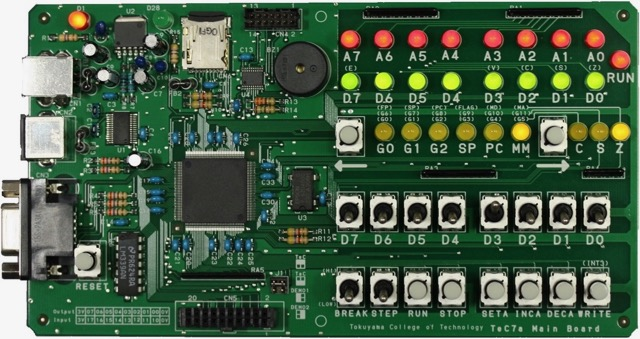
\includegraphics[scale=0.35]{Photo/TeC7.jpg}\\
(a) TeC7の写真
\end{center}
\end{minipage}
\begin{minipage}{0.38\columnwidth}
\begin{center}
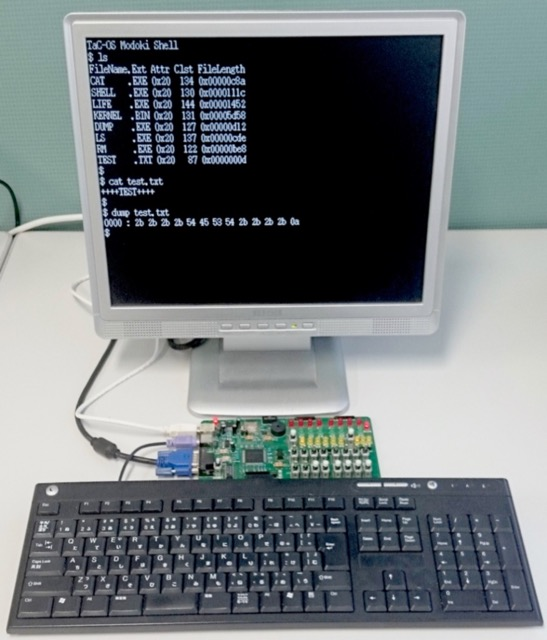
\includegraphics[scale=0.29]{Photo/TaC.jpg}\\
(b) TaCとしての使用例
\end{center}
\end{minipage}
\end{myfig}

TaC上では{\cmm}言語\footnote{
C言語に似た言語,
詳細は\url{https://github.com/tctsigemura/C--/blob/master/doc/cmm.pdf}を
参照のこと.}で記述されたTacOS\footnote{
詳細は\url{https://github.com/tctsigemura/TacOS}を参照のこと.} が動作する.
本書ではTacOSをオペレーティングシステムの実装例として参照する.

\subsection{ハードウェア構成}
\figref{tacBlock}にTaCのハードウェア構成を示す.
16ビットのシングルプロセッサ(CPUが一つ),
主記憶64KiBの非常に単純なシステムである.
単純なのでオペレーティングシステムの構築も容易である.
TaCに関する資料を付録\ref{appTac}にまとめる.

\myfigure{btp}{scale=0.48}{Fig/tacBlock-crop.pdf}
{TaCのハードウェア構成}{tacBlock}

\begin{itemize}
\item {\bf コンソールパネル} \\
\figref{tacPhoto}「(a) TeC7の写真」で,
TeC7本体右半分のランプやスイッチで構成される部分をコンソールパネルと呼ぶ.
コンソールパネルはCPUや主記憶と直接接続されており,
CPUを停止した状態で,
CPUや主記憶の内容を操作したり観察したりすることができる.
また,機械語命令を一命令毎に実行するステップ実行機能や,
ある番地の命令を実行した時点でプログラムを停止する
ブレーク機能ポイントが利用できる.
コンソールパネルの機能はハードウェアで実現されているので,
オペレーティングシステムの内部をステップ実行することも可能である.
TacOSの開発では,コンソールパネルがデバッグに活用された.

\item {\bf CPU} \\
\figref{tacRegPsw}に示すようなCPUレジスタとPSWを持つ16ビットCPUである.
PSWのフラグに実行モードを表すPビットを持ち,
カーネルモードとユーザモードを切り換えることができる.
機械語命令は,\figref{tacInsTbl}に示す46種類が準備されている.
機械語命令のアドレッシングモードは8種類ある.

\item {\bf メモリ} \\
メモリは\figref{tacMap}に示す構成である.
メモリ空間全体で64KiB,
自由に使用できるメモリが56KiB,
2KiBのVRAMと4KiBのIPL,32Bの割込みベクタからなる.
メモリは8ビット単位,または,16ビット単位で読み書きできる.
16ビット単位の場合は偶数アドレスを用いる.

\item {\bf タイマー} \\
$1$ミリ秒から$2^{16}-1$ミリ秒までの間隔で割込みを発生する
インターバルタイマーが二つ利用可能である.

\item {\bf ディスプレイアダプタ} \\
80文字×24行の文字をVGAディスプレイに表示する.
メモリ空間の{\tt E000h}から配置されるVRAMに書き込んだ
ASCIIコードと対応する文字をディスプレイに表示する.
{\tt E000h}番地がディスプレイの左上隅に対応する,
{\tt E001h}番地が一行目の2文字の位置,
{\tt E04Fh}番地が一行目の80文字の位置,
{\tt E050h}番地が二行目の1文字の位置に対応する.

\item {\bf SPIホストコントローラ} \\
スロットに挿入されたμSDカードをSPIモードに切換え読み書きを行う.
SPIホストコントローラに初期化コマンドを発行すると,
μSDカードをSPIモードに切換える.
ブロックアドレスとメモリアドレスを設定して読み出しコマンドを発行すると,
μSDカードの指定したブロックから512バイトのデータを
CPUを介さずに(DMA:Direct Memory Accessを用いて)メモリに読み出す.
書込みコマンドを発行すると,
メモリから指定ブロックにデータを書き込む.

\item {\bf シリアル通信インタフェース} \\
調歩同期方式,9,600Baudの通信インタフェースである.
USBシリアル変換ICを通してPC等のシリアルターミナルと通信できる.
1バイト転送する毎に割込みを発生する.

\end{itemize}

\subsection{TacOS}
\myfigure{btp}{scale=0.66}{Fig/tacosOrganization-crop.pdf}
{TacOSの構成}{tacosOrganization}

\figref{tacosOrganization}にTaC用のOSであるTacOSの構造を示す.
マイクロカーネルがプロセス間通信(IPC)機能を提供し,
サーバプロセスがメモリ管理やファイルシステム機能を提供する.
\figref{microkernel}の一般的なマイクロカーネル方式と異なり,
サーバプロセスがカーネルモードで動作しハードウェアに直接アクセスする.
また,サーバプロセスはマイクロカーネルと同じアドレス空間で動作するので,
カーネル内ルーチンをCALL機械語命令で直接に呼び出すことができる.

割込みやSVC命令の実行が原因で,
ユーザプロセスはカーネルモードに切り換わり
マイクロカーネル内の割込みハンドラが呼び出される.
割り込みハンドラで割込み原因を判断し,
マイクロカーネル内のルーチンを呼び出したり,
サーバプロセスの機能をIPCを用いて呼び出したりする.

\section{もう一つの仮想マシン}

\ref{osRole}で述べたように,
オペレーティングシステムは抽象化され便利な拡張マシン(仮想マシン)を,
必要な数だけ提供する.
ここで述べた仮想マシンは,単一ユーザ・プロセスの実行環境のことである.
同じ「仮想マシン」と言う用語が,
オペレーティングシステムを実行することが可能な,
よりハードウェアを忠実に再現した仮想マシンを指す場合もある.
ここでは,
一台のコンピュータ上で複数のオペレーティングシステムを実行可能な,
もう一つの仮想マシンについて紹介する.

\subsection{Type 2 ハイパーバイザ}
例えば,
Macを使用している人がWindowsでしか動作しないアプリケーションを使用する
場合を想像してしてみる\footnote{
徳山高専情報電子工学科のパソコン室では,
WindowsやLinuxでしか動作しないXilinx ISE WebPACKをMacで使用している.}.
予めMacのハードディスクにmacOSとは別にWindowsもインストールしておき,
電源投入時にmacOSとWindowsを選んでブートする方法もあるが,
オペレーティングシステムを切換える度にコンピュータを再起動するのは不便である.
また,macOSのアプリケーションとWindowsのアプリケーションを同時に実行したい
場合もある.

そこで,\figref{type2Hypervisor}に示すような
「Type 2 ハイパーバイザ(Type 2 Hypervisor)」を用いた仮想化が用いられる.
ハイパーバイザは
{\bf ホスト・オペレーティングシステム}の一つのユーザプロセスとして実行され,
コンピュータ一台の機能をエミュレーションする.
ハイパーバイザがエミュレーションするコンピュータの中で,
{\bf ゲスト・オペレーティングシステム}が稼働する.
エミュレーションはソフトウェアだけで完全に行うのではなく\footnote{
完全にソフトウェアで行う場合もある.},
ハードウェアの支援を受けて行うので高速に行うことができる\cite{virtualization}.
Type 2 ハイパーバイザとして有名は製品は,
VMware Workstation,
VMware Fusion,
VirtualBox\footnote{
徳山高専情報電子工学科のパソコン室では
macOS上のVirtualBoxでWindowsを動作させている.
%このWindowsの中でXlinix ISE WebPACKが使用できる.
}等である.

\myfigure{btp}{scale=0.66}{Fig/type2Hypervisor-crop.pdf}
{Type 2 ハイパーバイザ}{type2Hypervisor}

\subsection{Type 1 ハイパーバイザ}
メインフレーム上で1960年代から使用されている方式である.
現在ではPCサーバの仮想化にも使用されている.
Type 1 ハイパーバイザはホスト・オペレーティングシステム無しに
ハードウェア上で直接実行される.
Type 1 ハイパーバイザとして有名な製品は,
IBM z/VM,
VMware vSphere,
Xen,
Hyper-V等である.

サーバ向けの製品が主流であり,
例えば VMware vSphere は
実行中のゲストを他の物理サーバに移動する等,
非常に高度な機能を持っており\cite{vsphere},
一台のサーバ上に効率よく多数の仮想マシンを動かすことができる.
徳山高専情報電子工学科のパソコン室でも,
2台のサーバ上に50台の仮想デスクトップマシンを動かしていたことがある.

\myfigure{btp}{scale=0.66}{Fig/type1Hypervisor-crop.pdf}
{Type 1 ハイパーバイザ}{type1Hypervisor}

\subsection{仮想アプライアンス}
ゲスト・オペレーティングシステムとアプリケーションまでインストールし,
すぐに使用できる状態で配布される仮想マシンである.
例えば,メールフィルタソフトをインストールした仮想マシンを
入手しハイパーバイザで実行するだけですぐにメールフィルタリングが開始できる.

同じ手法で,
すぐに使用できるパーソナルコンピュータ用の
デスクトップ・オペレーティングシステムが配布されている場合もある.
Linux の一種であるUbuntuの場合,
VirtulBoxですぐに実行できるディスクイメージがダウンロードできる\cite{ubuntu}.
仮想アプライアンスは,
ソフトウェアの新しい流通手法である.

\section{まとめ}
本書は{\bf SMP(対称型マルチプロセッシング:Symmetric Multiprocessing)}の
コンピュータを前提にしている.
CPUは{\bf PSW(Program Status Word)}と{\bf CPUレジスタ}を含んでいる.
最近のIntel社のCPUでは,従来のCPUを{\bf Core(コア)},
複数のコアを含んだLSIのことをCPUと呼ぶ.

オペレーティングシステムのカーネルは,
割込みハンドラ,ディスパッチャ,サービスモジュール,
デバイスドライバ等から構成される.
ユーザ・プロセスからカーネルへの切換え原因は{\bf 割込み}だけである.
ユーザ・プロセス毎に{\bf 仮想CPU},{\bf 仮想メモリ空間},管理情報等を
持っている.

カーネルの構成方式には,
{\bf 単層カーネル(モノリシック・カーネル)}方式と
{\bf マイクロカーネル(micro-kernel)}方式の二種類があった.
マイクロカーネル方式ではサービスモジュールをサーバ・プロセスとし,
{\bf IPC(プロセス間通信)}を用いてサービスを要求する.
サービスモジュール間の独立性が高くなり高信頼性のシステムを構成可能であるが,
IPCはオーバーヘッドが大きい.
信頼性と性能はトレードオフの関係にある.

{\bf TaC}は,本書でオペレーティングシステムの実装例として使用する
TacOSを稼働させるコンピュータである.
コンソールパネルを持ち,
TacOSのカーネル内までステップ実行によるトレースが可能である.
{\bf TacOS}はマイクロカーネル方式の簡単なオペレーティングシステムである.
本書では,しばしばTacOSのソースコードを実装例として参照する.




 % 前提知識
\part{CPU管理}
\chapter{CPUの仮想化}
オペレーティングシステムは,
ハードウェアを抽象化した使いやすい拡張マシン(仮想マシン)を
必要な数だけ提供する.
数に限りがある資源は,必要な数だけあるように見せるために仮想化が行われる.
CPU資源も仮想化し,各プロセスが自分専用のCPUを持っているように見せかける.

%==============================================================================
\section{時分割多重}
CPUを仮想化するためには時分割多重が用いられる.
ハードウェアである実CPUの数は限られているので,
時間を区切って実CPUを使用するプロセスを次々に切換えていく.
\figref{virtualCPU}にCPU仮想化の原理を示す.

\begin{myfig}{btp}{時分割多重によるCPUの仮想化}{virtualCPU}
  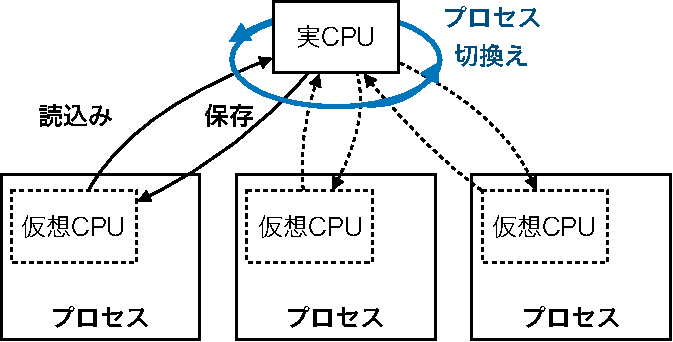
\includegraphics[scale=0.7]{Fig/virtualCPU-crop.pdf}
\end{myfig}

実CPUは\figref{cpuBlock}のような構造をもつハードウェアである.
プロセスの構造は\figref{procOrganization}に示した通りであり,
仮想CPUを含んでいる.
実CPUが短時間(例えば10ms)に次々と実行するプロセスを切換えていくことで,
複数のプロセスが夫々に専用のCPUを持ち並行して実行されているように見せかける.

CPUが実行するプロセスを切り換えるには,まず,
実CPUのコンテキストを現在のプロセスの仮想CPU領域に保存する.
次に,新しく実行するプロセスの仮想CPU領域から実CPUにコンテキストを読込み,
新しいプロセスの実行を再開する.
一つのプロセスから別のプロセスに切換える処理を
\emph{コンテキストスイッチ}と呼ぶ.
また,実CPUにコンテキストを読込んで実行を再開することを\emph{ディスパッチ},
ディスパッチを行うプログラムを\emph{ディスパッチャ}と呼ぶ.
\figref{osOrganization}にもディスパッチャは描かれていた.

%==============================================================================
\section{プロセスの状態}
\label{procState}
プロセスは,
キーボード等の入出力装置からの入力を待つ状態になったり,
時間が経過するのを待つ状態になったりする.
\emph{待ち(Waiting)状態}のプロセスにはCPUを割当てる必要がない.
このようにプロセスは幾つかの状態を持っている.
プロセスの状態はUNIXではpsコマンドで確認できる.
プロセスを模式的に示した\figref{procOrganization}では,
「プロセス情報」の「プロセスの状態」のことである.

\subsection{基本的な三つの状態}
\figref{procState}にプロセスの状態遷移図を示す.
この図は最も簡単なものであり,
実際のオペレーティングシステムでは,
もっと状態数が多くなる\footnote{
  macOSのpsコマンドのオンラインマニュアルで確認すると,
  macOSではプロセスの状態が,
  I(Idle),
  R(Runnable),
  S(Sleep),
  T(sTopped),
  U(Uninterruptible wait),
  Z(Zombie)の六つであることが分かる.}.
図に示された三つの状態を説明する.

\begin{itemize}
\item \emph{Ready(実行可能)} \\
  CPUを割当てれば実行を開始できる状態のことである.
  プロセスはCPUが割当てられるのを待っている.
\item \emph{Running(実行中)} \\
  CPUが割当てられ実行している状態のことである.
  CPUの数より多くのプロセスが同時にRunningになることはできない.
\item \emph{Waiting(待ち)} \\
  シグナルの到着や入出力の完了等の事象(イベント)を待っている状態である.
  プロセスは実行することができない.
\end{itemize}

\begin{myfig}{btp}{プロセスの状態遷移}{procState}
  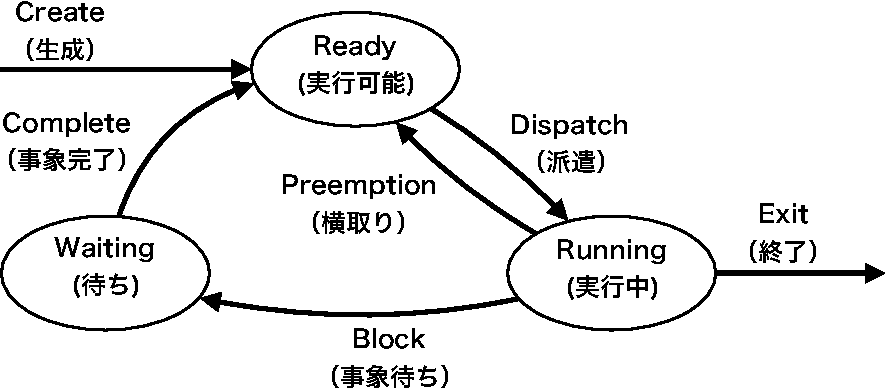
\includegraphics[scale=0.66]{Fig/procState-crop.pdf}
\end{myfig}

\subsection{状態遷移}
\figref{procState}に示された六つの状態遷移の意味は以下の通りである.

\begin{enumerate}
\item \emph{Create(クリエート,生成)} \\
  新しいプロセスが生成されるとReady状態になる.
  親プロセスが\|fork()|システムコール(UNIXの場合)や
  \|CreateProcess()|システムコール(Windowsの場合)を実行すると,
  新しい子プロセスが生成される.
\item \emph{Dispatch(ディスパッチ,派遣)} \\
  Ready状態のプロセスは,
  自分の順番が来たらCPUが割当てられRunning状態に遷移し実行を開始する.
\item \emph{Preemption(プリエンプション,横取り)} \\
  Running状態のプロセスは,
  決められた時間(クオンタムタイム)を使い切ったときや,
  より優先度の高いプロセスがReady状態になったとき,
  CPUを取り上げられReady状態に遷移する.
\item \emph{Block(ブロック,事象待ち)} \\
  Running状態のプロセスが,
  システムコールを発行して自らWaiting状態に遷移することがある.
  例えば入出力システムコール
  (\|open()|,\|read()|,\|write()|,\|close()|等)や,
  シグナル待ちシステムコール(\|pause()|,\|wait()|,\|sleep()|等)
  を発行した場合である.
  また,他のプロセスからシグナルを受信した場合も,
  Waiting状態に遷移することがある.
  更に,仮想記憶の機能を持つオペレーティングシステムでは,
  プロセスが読み書きしようとした領域がメモリ上に存在しない時も
  この遷移が起こり,
  メモリ領域を確保するための処理がカーネル内部で始まる.
\item \emph{Complete(コンプリート,事象完了)} \\
  Waiting状態のプロセスは,
  入出力の完了やシグナルの発生等の事象(イベント)が発生すると
  Ready状態に遷移する.
  Waiting状態のプロセスは停止しているのでプロセスが事象を発生することはない.
  事象はプロセスの外部からもたらされる.
\item \emph{Exit(終了)} \\
  プロセスが自ら\|exit()|システムコール(UNIXの場合)や
  \|ExitProcess()|システムコール(Windowsの場合)を用いて終了する場合,
  または,プロセスがシグナルを受ける等して終了させられる場合に,
  この遷移が起こる.
  シグナルはプロセス(他プロセス,自プロセス)から明示的に送信される場合と,
  自プロセスが保護違反などのエラーを起こして発信される場合がある.
\end{enumerate}

%==============================================================================
\section{プロセスの切換え(コンテキストスイッチ)}
Running状態のプロセスがBlock遷移またはPreemption遷移しCPUを取り上げられると,
他のReady状態のプロセスがCPUを割付けられDispatch遷移し実行を再開する.

\subsection{切換えの原因}
Running状態のプロセスが状態遷移を起こす原因を以下にまとめ直す.

\begin{enumerate}
\item イベント \\
  Running状態のプロセスは,
  自ら「システムコールを発行」することでBlock遷移をすることがある.
  また,他のプロセスからの「\emph{干渉}\footnote{
      干渉には,より優先順位の高いプロセスが実行可能になった,
      別のプロセスからシグナル等を受取った等がある.}
    を受け」Block遷移することがある.
\item タイムスライシング \\
  Running状態のプロセスが長時間の実行を続けるとPreemption遷移をする.
  一度に実行しても良い時間(クオンタムタイム)を使い切ったためである.
  Ready状態のプロセスが他にあれば,そのプロセスに実行が切換わる.
  他に実行すべきプロセスが無い場合は,再度,同じプロセスが実行される.
\end{enumerate}

\subsection{切換え手順}
\figref{procSwitch}に二つのプロセス間で実行が切り換わる様子を示す.
図では時間に従って上から下へ処理が進む.
左側はプロセスAの実行を,
右側はプロセスBに実行を,
中央はカーネルの実行を表している.
以下では,
図の上半分でプロセスAからプロセスBに実行が切り替わる手順を説明する.
図の下半分の説明は省略するが,
上半分と同様な手順でプロセスBからプロセスAに切り替わる手順を示している.

\begin{myfig}{btp}{プロセスの切換え}{procSwitch}
  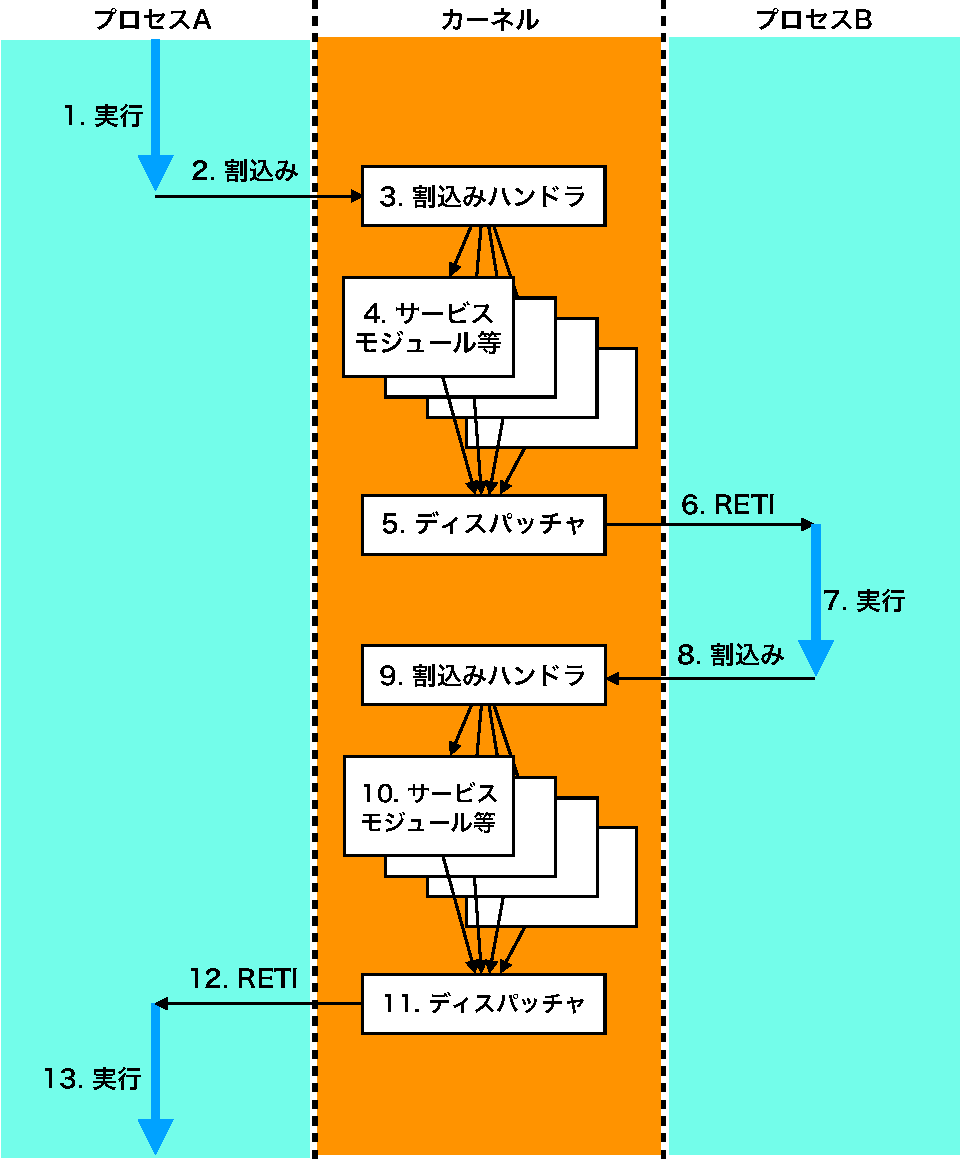
\includegraphics[scale=0.6]{Fig/procSwitch-crop.pdf}
\end{myfig}

\begin{enumerate}
\item 実行 \\
  日頃はCPUがユーザ・プロセスを実行している.
\item 割込み \\
  割込みが発生し処理がプロセスAからカーネル内の割込みハンドラに移る.
  割込みの原因は\ref{interruptSource}で述べた様々なものが考えられる.
  割込みが発生すると以下の処理が\emph{CPUのハードウェアにより自動的に}される.
  \begin{enumerate}
  \item CPUの(PCを含む)PSWがスタックに保存される.
  \item CPUの実行モードがカーネルモードに切り換わる.
  \item 割込みハンドラにジャンプする.
  \end{enumerate}
\item 割込みハンドラ \\
  PSW(スタック上にある)とCPUレジスタ(\figref{cpuBlock}参照)からなる
  プロセスのコンテキストを
  プロセスの仮想CPU領域(\figref{procOrganization}参照)に保存する.
  次に割込み原因を調べ,
  割込み原因に応じた処理(サービスモジュール等)にジャンプする.
  例えば,
  割込み原因が\|open()|システムコールなら,
  openシステムコールの処理を行うファイルシステムの
  サービスモジュールにジャンプする.
  割込み原因がI/O完了なら,
  完了したI/Oに対応するデバイスドライバにジャンプする.
\item サービスモジュール等 \\
  サービスモジュールやデバイスドライバが割込み原因に応じた処理を行う.
  この過程でプロセスの状態が変化することがある.
  例えば,プロセスが発行したシステムコールが原因でBlock遷移する場合や,
  タイマーやI/Oの完了割込によりWaiting状態だった別のプロセスが
  Complete遷移する場合,
  タイマーの完了割込により現在のプロセスがPreemption遷移する場合等が
  考えられる.
  サービスモジュール等の処理が完了するとディスパッチャにジャンプする.
\item ディスパッチャ \\
  実行可能なプロセスの中から一つを選び,
  選んだプロセスの仮想CPU領域の内容をCPUレジスタにロードする.
  最後にPSWを復旧する機械語命令(RETI)を実行しプロセスの実行に戻る.
\item RETI \\
  PSWを復旧する機械語命令として
  割込復帰用の\emph{RETI(RETurn from Interrupt)命令}を用いる.
  RETI命令は単一の命令でPSW(PCとフラグ)を一度にスタックから復旧する.
  CPUの実行モードを表すフラグはPSWに含まれているので,
  PSWが復旧されることで実行モードがカーネルモードからユーザモードに切り換わる.
\item 実行 \\
  新しく選択されたユーザ・プロセスが実行される.
\end{enumerate}

\subsection{切換えの例}
計算に長い時間を要する二つのプロセスだけがある時,
クオンタムタイムを使い切ってもう一方のプロセスに切り換わり,
交互に実行される様子を\figref{procSwitchInst}に示す.
以下に手順を説明する.

\begin{myfig}{btp}{プロセスの切換えの例}{procSwitchInst}
  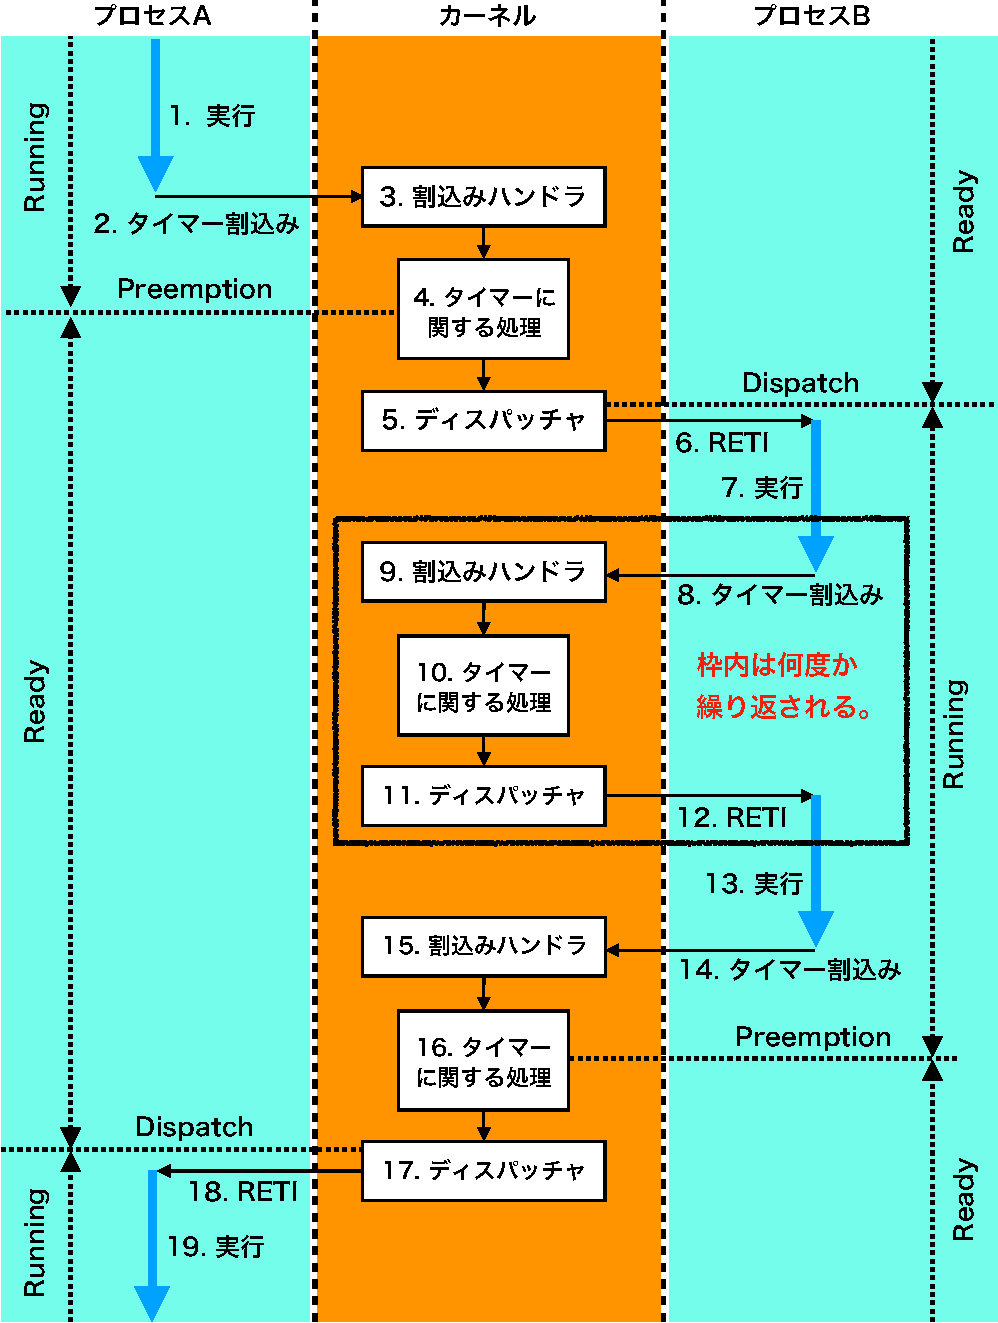
\includegraphics[scale=0.6]{Fig/procSwitchInst-crop.pdf}
\end{myfig}

\begin{enumerate}
\item 実行 \\
  プロセスAは計算処理を続けている.
  長い時間に渡ってシステムコールを発行することは無い.
\item タイマー割込み \\
  タイマーは一定間隔で割込みを発生する.
  割込が発生するとCPUのハードウェアが自動的にPSWを保存し,
  割込みハンドラにジャンプする.
  オペレーティングシステムは,
  主に,この割込みを基準に時間の経過を認識する.
\item 割込みハンドラ \\
  プロセスのコンテキストをプロセスの仮想CPUに保存する.
  その後,割込原因を調べタイマーからの割込みなので,
  「タイマーに関する処理」を行うカーネル内のモジュールへジャンプする.
\item タイマーに関する処理 \\
  一定間隔で発生するタイマーからの割込みを利用して,
  システムの時計を進めたり,
  リソース(CPUやメモリ等)の利用統計データを更新したりする.
  その間にプロセスAがクオンタムタイムを使い切ったことが判明すると,
  プロセスAをPreemption遷移させる.
  この時点でプロセスAの状態がReadyに変化する.
\item ディスパッチャ \\
  Ready状態のプロセスの中から適切な一つを選びDispatch遷移させる.
  \figref{procSwitchInst}はプロセスBが選択された場合である.
  ディスパッチャはプロセスBのCPUレジスタを復旧する.
\item RETI \\
  プロセスBのPSWを復旧し,プロセスBの実行を再開する.
\item 実行 \\
  プロセスBは計算処理を再開する.
  プロセスBも長い時間計算を続けるプロセスとする.
\item タイマー割込み \\
  計算を続けるうちにタイマーからの割込みが発生する.
\item 割込みハンドラ \\
  プロセスBのコンテキストを保存する.
\item タイマーに関する処理 \\
  プロセスBは,まだ,クオンタムタイムを使い切っていないので,
  Preemptionは発生しない.
\item ディスパッチャ \\
  Preemptionは発生しないので,
  プロセスBのコンテキストを復旧する.
\item RETI \\
  プロセスBに戻る.
\item 実行 \\
  プロセスBは計算処理を再開する.
\item タイマー割込み \\
  8.〜13. を何度か繰り返し,
  クオンタムタイムを使い切った時のタイマー割込みである.
\item 割込みハンドラ \\
  プロセスBのコンテキストを保存する.
\item タイマーに関する処理 \\
  クオンタムタイムを使い切ったのでPreemptionが発生する.
\item ディスパッチャ \\
  Ready状態のプロセスAを選択しDispatch遷移させる.
  プロセスAのコンテキストを復旧する.
\item RETI \\
  プロセスAに戻る.
\item 実行 \\
  プロセスAは計算処理を再開する.
\end{enumerate}

%==============================================================================
\section{PCB(Process Control Block)}
PCBはプロセスを表現する重要なカーネル内のデータ構造である.
PCBはカーネル内のプロセステーブルに格納される.

\subsection{PCBの内容}
PCBは,\figref{procOrganization}の
「仮想CPU」と「プロセス情報」を合わせたものに相当する.
PCBには以下のような情報が格納される.

\begin{itemize}
\item 仮想CPU
\item プロセス番号
\item 状態(Running,Waiting,Ready等)
\item 優先度
\item 統計情報(CPU利用時間等)
\item 次回のアラーム時刻
\item 親プロセス
\item 子プロセス一覧
\item シグナルハンドリング
\item 使用中のメモリ
\item オープン中のファイル
\item カレントディレクトリ
\item プロセス所有者のユーザ番号
\item PCBのリストを作るためのポインタ
\end{itemize}

\subsection{PCBリスト}
カーネル内ではPCBがプロセスを表現する.
例えば,優先順にソートされたReady状態のプロセスのリストは,
優先度をキーにソートされたPCBの線形リスト(\emph{待ち行列})として表現される.
この線形リストを\emph{実行可能列}と呼ぶ.
その様子を\figref{procQueue}に示す.
図は,数値が小さいほど優先度が高い意味になっている.

\begin{myfig}{btp}{PCBのリスト}{procQueue}
  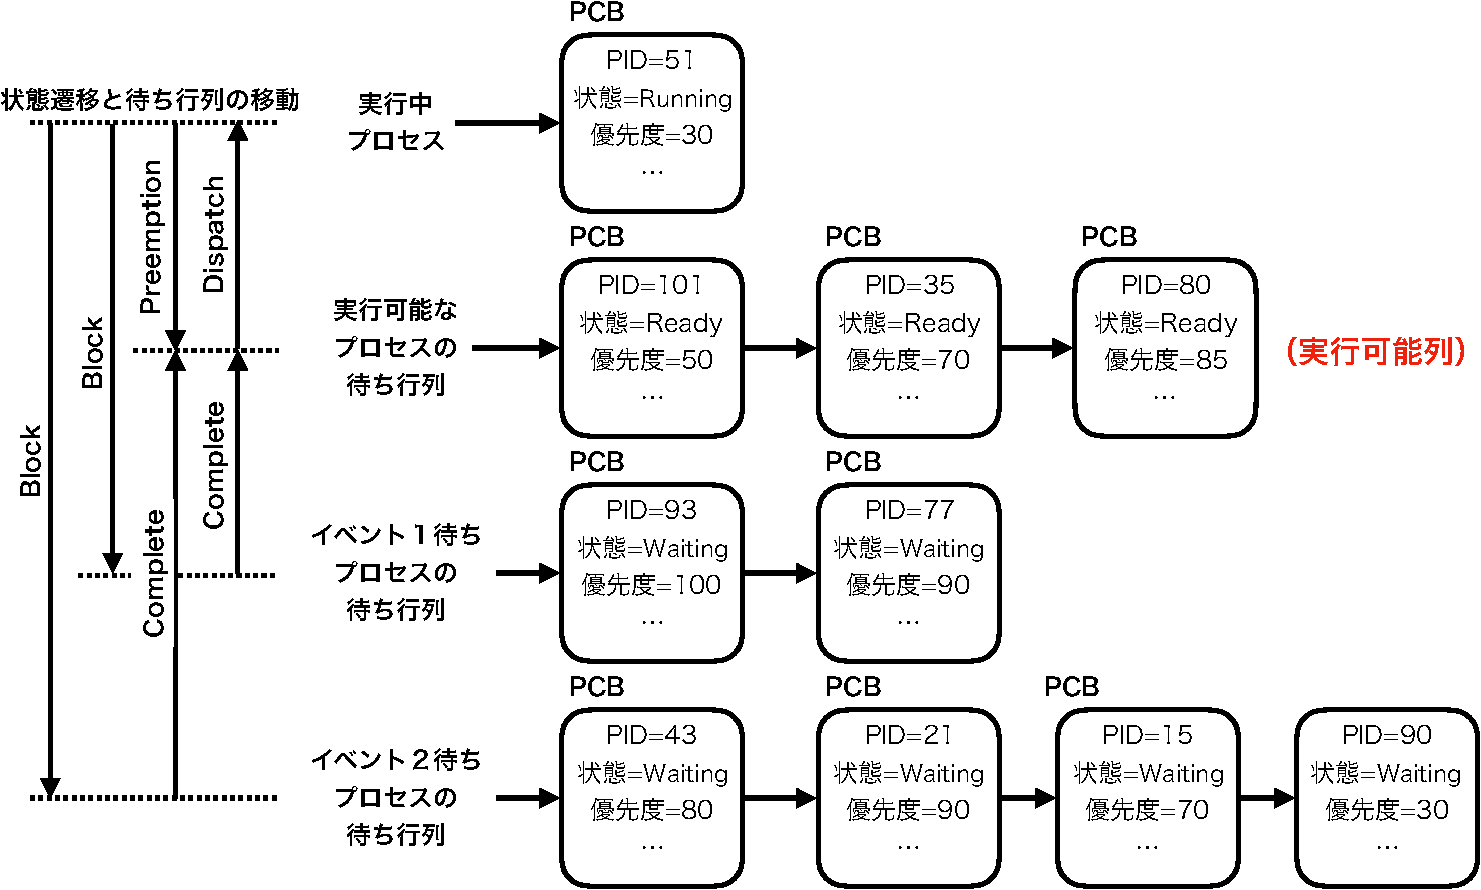
\includegraphics[scale=0.55]{Fig/procQueue-crop.pdf}
\end{myfig}

Ready状態のプロセスだけでなく,
Running状態のプロセスや,
Waiting状態のプロセスも待ち行列で管理される.
Waiting状態のプロセスは,
待ち合わせているイベント毎に待ち行列を作っている.
イベント待ち行列のソート順はイベント毎にルールが決められる.

プロセスの状態遷移に合わせてPCBが待ち行列の間を移動する.
\figref{procQueue}の左側の「状態遷移と待ち行列の移動」が
「どの待ち行列から,どの待ち行列に移動可能か」を表している.
例えば,Running状態(実行中)のプロセスがPreemption遷移をすると,
状態がReadyに変わるだけでなく,
PCBが「実行可能なプロセスの待ち行列」に移動する.
この移動ルールは\figref{procState}の状態遷移と一致している.

%==============================================================================
\section{スレッド(Thread)}
ここまで,一つのプロセスが一つの仮想CPUを持つモデルを考えてきた.
しかし,実際のコンピュータハードウェアはCPUを複数持つSMPの場合もある.
これでは
「ハードウェアの機能を抽象化した便利な\emph{拡張マシン}」
(\ref{abstruction}参照)であるはずのプロセスが,
「CPUが一つしかない\emph{縮小マシン}」なっている.
そこで,SMPに対応しプロセスが複数の仮想CPUを持つモデルを導入する.
これにより,一つのプロセスが
並列実行する複数の処理の流れ(スレッド)を持つことが可能になる.

\subsection{スレッドの役割}
複数のプロセス(ジョブ)を主記憶にロードしておくことで
CPUの利用効率を高くできることは既に説明した
(\pageref{multiprogramming}ページ,マルチプログラミング参照).
マルチプログラミングの,もう一つのメリットは,
プログラミングが簡単になる場合があることである.
以下ではWebサーバを例に,
マルチプログラミングによる改善を紹介する.

\begin{itemize}
\item マルチプロラミングなし \\
  \figref{singleProcSingleClient}に最も簡単なモデルを示す.
  Webサーバはリクエストを受信すると,それに対するレスポンスを返す.
  処理は1番目のクライアントから順に行われ,
  2番目のクライアントは1番目の処理が終了するまで待たされる.
  このモデルの問題点は,
  処理中にWebサーバプロセスがI/O待ち等でブロック(Block)する可能性があり,
  その間,他のクライアントへのサービスがされないことである.

  2番目以降のクライアントが長時間待たされないように,
  複数のクライアントの処理を並行してできるように改良したモデルが
  \figref{singleProcMultiClient}である.
  「I/O完了の監視」は通信を含む複数の入出力を同時に監視し,
  どれかが読み書き可能になるのを待つ機能である.
  UNIXでは\|select()|システムコールがこの機能を持つ.
  読み書き可能になったことを確認後に読み書きを行うので
  プロセスがブロックすることが無くなり,
  複数のクライアントに対して同時にサービスを行うことができる.

  しかし,Webサーバのプログラミングは難しくなる.
  一方のクライアントの処理が終わらないうちに,
  別のクライアントの処理を開始する必要があるからである.
  クライアント毎に処理がどこまで進んでいるのかを表す
  \emph{状態}を持つ必要がある.
  また,CPUが複数存在する場合でも,
  同時には一つのCPUしか働かないことも問題である.

  \begin{myfig}{btp}{マルチプログラミングを用いないWebサーバ}
    {singleProcSingleThread}
    \begin{minipage}{0.49\columnwidth}
      \begin{center}
        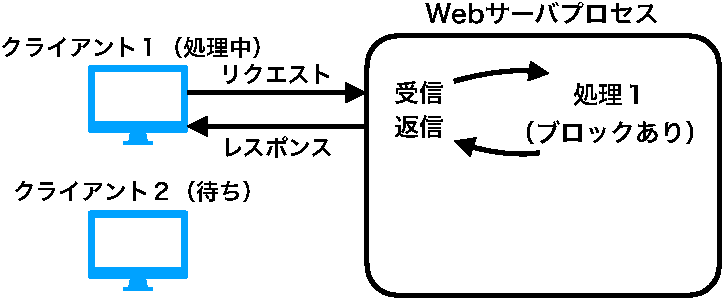
\includegraphics[scale=0.6]{Fig/singleProcSingleClient-crop.pdf}
        \subcaption{最も基本的なWebサーバのモデル}
        \label{fig:singleProcSingleClient}
      \end{center}
    \end{minipage}
    \begin{minipage}{0.49\columnwidth}
      \begin{center}
        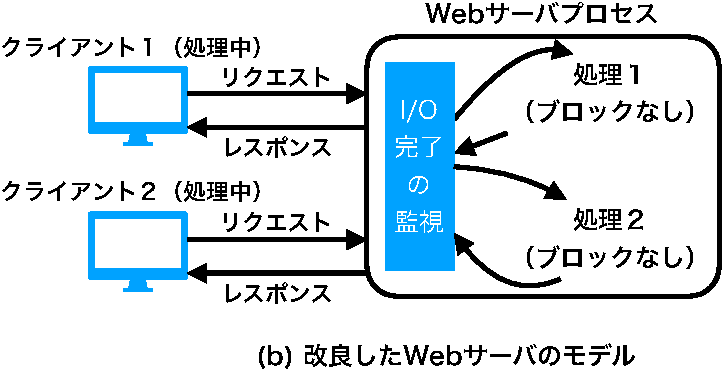
\includegraphics[scale=0.6]{Fig/singleProcMultiClient-crop.pdf}
        \subcaption{改良したWebサーバのモデル}
        \label{fig:singleProcMultiClient}
      \end{center}
    \end{minipage}
  \end{myfig}
  
\item マルチプロセス \\
  マルチプログラミングを用いることで前記の問題を解決したモデルを
  \figref{multiProc}に示す.
  Webサーバプロセスは,
  まず,接続要求を待ちクライアント1からの接続を受け入れる.
  次に,クライアント1専用のサーバプロセスを生成し処理を任せる.
  Webサーバプロセスは,
  生成したプロセスの終了を待たずに,
  次の接続要求待ちになる.
  クライアント2からの接続要求があったら
  クライアント2専用のサーバプロセスを生成し,
  接続要求待ちに戻る.

  このモデルなら,
  各クライアントの処理を別々のプロセスが行っているので,
  プロセスがブロックしても構わない.
  そのため,プログラミングは簡単になる.
  また,CPUが複数あればプロセスが真に並列に実行される.
  しかし,プロセスの生成はメモリ空間の確保や初期化を含み\emph{重い処理}である.
  また,
  プロセスはメモリを共有していないのでプロセス間の情報共有には効率が悪い.

\item マルチスレッド \\
  複数のスレッドを使用したモデルを\figref{multiThread}に示す.
  マルチプロセスの場合と良く似たプログラムであるが,
  クライアント毎に専用のプロセスを作る代わりに,
  クライアント毎に専用のスレッドを作る.
  スレッドの生成はプロセス生成より10〜100倍速いと
  言われている\cite{lightWeight}.
  また,スレッドはメモリを共有しているので情報共有には都合が良い.
  例えば,Webサーバが頻繁に参照されるページをメモリ上にキャッシュする場合,
  キャッシュをスレッドで共有できる.

  \begin{myfig}{btp}{マルチプログラミングを用いるWebサーバ}{multiPrograming}
    \begin{minipage}{0.49\columnwidth}
      \begin{center}
        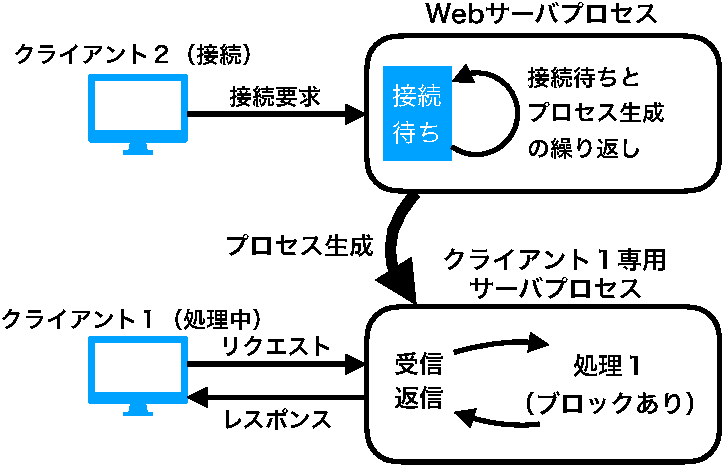
\includegraphics[scale=0.6]{Fig/multiProc-crop.pdf}
        \subcaption{マルチプロセスにしたWebサーバのモデル}
        \label{fig:multiProc}
      \end{center}
    \end{minipage}
    \begin{minipage}{0.49\columnwidth}
      \begin{center}
        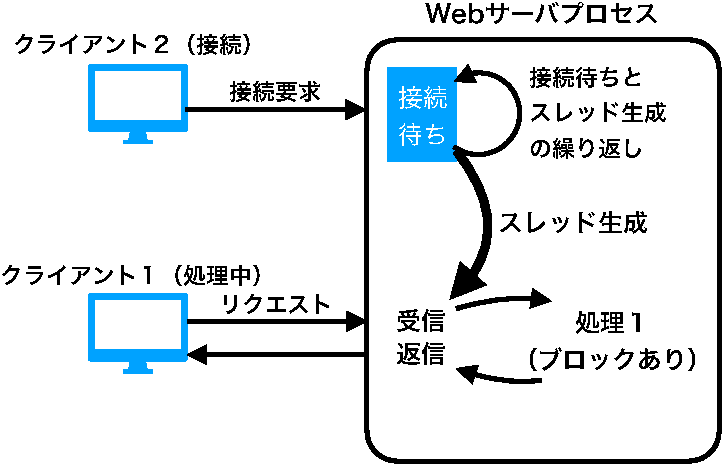
\includegraphics[scale=0.6]{Fig/multiThread-crop.pdf}
        \subcaption{改良したWebサーバのモデル}
        \label{fig:multiThread}
      \end{center}
    \end{minipage}
  \end{myfig}
\end{itemize}

\subsection{スレッドの形式}
読者は,「スレッドはカーネルが実現する」と暗黙のうちに考えていたかも知れない.
しかし,ユーザプログラム(ライブラリ)内でスレッドを実現することもある.
カーネルが実現するスレッドを\emph{カーネルスレッド},
ユーザプログラム内で実現するスレッドを\emph{ユーザスレッド}と呼ぶ.

\begin{myfig}{btp}{ユーザスレッドとカーネルスレッド}{threadOrganization}
  \begin{minipage}{0.49\columnwidth}
    \begin{center}
      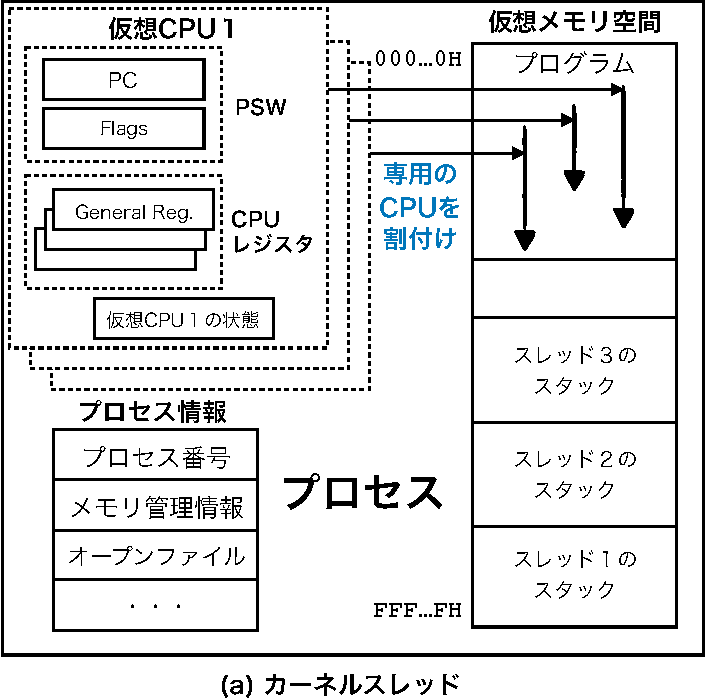
\includegraphics[scale=0.6]{Fig/kernelThread-crop.pdf}
      \subcaption{カーネルスレッド}
      \label{fig:kernelThread}
    \end{center}
  \end{minipage}
  \begin{minipage}{0.49\columnwidth}
    \begin{center}
      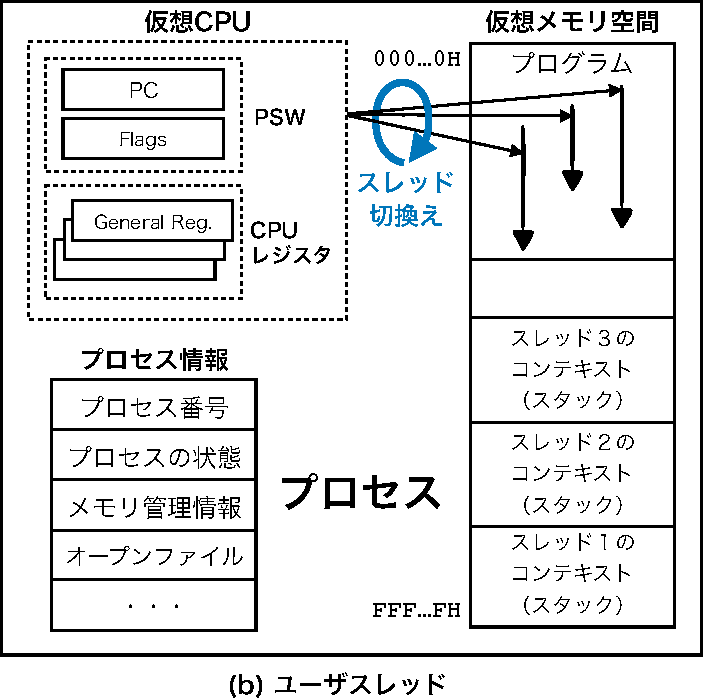
\includegraphics[scale=0.6]{Fig/userThread-crop.pdf}
      \subcaption{ユーザスレッド}
      \label{fig:userThread}
    \end{center}
  \end{minipage}
\end{myfig}

\begin{itemize}
\item \emph{カーネルスレッド} \\
  カーネルスレッドの模式図を\figref{kernelThread}に示す.
  カーネルスレッドはプロセスの仮想CPUを複数にし,
  仮想CPUがプログラムを並行して実行する.
  「プロセス情報」から「プロセスの状態」は無くなり,
  代わりに仮想CPU毎に「仮想CPUの状態」を管理するようになる.
  CPUが複数ある時,カーネルスレッドであれば,
  プロセス内を真に並列実行することが可能である.
\item \emph{ユーザスレッド} \\
  ユーザスレッドの模式図を\figref{userThread}に示す.
  プロセスには単一の仮想CPUしかない.
  ユーザスレッドは仮想CPUを時分割多重して実現される.
  カーネルを経由しないでスレッドの生成や切換えをすることができるので,
  オーバーヘッドが非常に小さい.
\end{itemize}

以下に述べるように,両者を組合せた三つのスレッドモデルが使用される.

\begin{enumerate}
\item \emph{One-to-One Model} \\
  全てのスレッドがカーネルスレッドのモデルである.
  \figref{kernelThread}に相当する.
  プロセス内にカーネルが管理する仮想CPUが複数あるので,
  複数プロセスと同等な並列実行が可能である.
  しかし,スレッドの生成や切換えにカーネルが介入するので,
  処理は重くなる.
  また,システムによっては生成できるスレッド数に制限がある.
\item \emph{Many-to-One Model} \\
  複数(Many)のユーザスレッドを
  一つ(One)のカーネルスレッドで実行するモデルである.
  \figref{userThread}に相当する.
  プロセス内にカーネルスレッドは一つしか存在しない.
  ユーザスレッドはユーザプログラム(ライブラリ)の工夫で
  単一のカーネルスレッドを複数に見せかけているだけなので,
  真の並列実行にはならない.
  また,何れかのスレッドがシステムコールでブロックすると,
  全てのスレッドが停止してしまう問題がある.
\item \emph{Many-to-Many Model} \\
  複数の(Many)のユーザスレッドを
  複数の(Many)のカーネルスレッドで実行するモデルである.
  カーネルスレッドの数をユーザスレッドの数より多くすることはない.
  前記二つのモデルの折衷案である.
\end{enumerate}

\subsection{スレッドプログラミング}
配列データの合計を求める処理をスレッドを用いて高速化する例を考えよう.
\figref{threadedSum}に原理を示す.
配列\|a|をM分割し個別スレッドで(CPUが複数あれば)同時に小計を計算する.
小計は配列\|total|に格納する.
最後に\|main|スレッドが\|total|の合計を求めると全体の合計\|sum|が計算できる.

\begin{myfig}{btp}{M個のスレッドで手分けして合計を計算する様子}{threadedSum}
  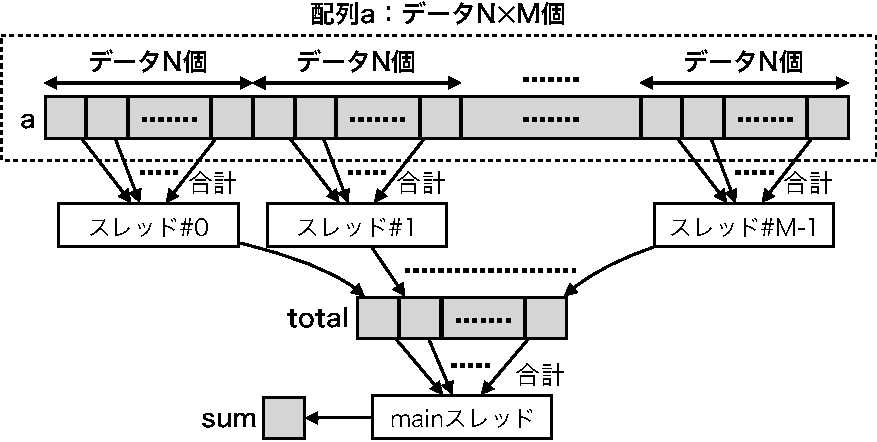
\includegraphics[scale=0.66]{Fig/threadedSum-crop.pdf}
\end{myfig}

\subsubsection{POSIXスレッドによる実装}
このアイデアをPOSIXスレッド\footnote{
  POSIXスレッドはUNIX系のオペレーティングシステムで使用できる.
}を用いたC言語プログラムにしたものをリスト\ref{threadTest}\footnote{
  このプログラムは macOS High Sierra で動作確認をした.
}に示す.

\lstinputlisting[numbers=left,float=btp,label=threadTest,
  caption=M個のスレッドで分担して配列データの合計を求めるプログラム]
  {SampleCode/pThread/threadTest.c}

12行の\|thread()|関数はM個のスレッドで同時に並列実行される.
配列\|a|の担当範囲等は引数\|arg|により指示される.
関数の引数(\|arg|)やローカル変数(\|args|,\|sum|,\|i|)は,
スレッドのスタック(\figref{threadOrganization}参照)に割付けられるので,
スレッド毎に別の実体を持つ.
グローバル変数\|a|や\|total|等は全てのスレッドで共有される.

32行の\|pthread_attr_init()|は引数の\|pthread_attr_t|型変数を
デフォルトのアトリビュート値で初期化する.
33行の\|pthread_create()|がスレッドを生成する関数である.
新しいスレッドの実行は引数で指定された\|thread()|関数から始まる.
\|pthread_create()|の引数\|p|は,
\|thread()|関数が実行を開始する時に\|arg|引数に渡される.

38行の\|pthread_join()|はスレッドの終了を待つ関数である.
スレッドの終了が確認できたら,39行で小計を\|sum|に足し込む.

\subsubsection{実行時間の計測結果}
リスト\ref{threadTest}のプログラムの実行時間を\tabref{threadTimeTbl}に,
グラフにしたものを\figref{threadTimeGrph}に示す
\footnote{
  実行時間の計測にはOS X の \texttt{time} コマンドを用いた.
}
\footnote{
  実行時間が短すぎて比較し難いので,
  プログラムの14行から17行を10万回繰り返すように改造した上で計測した.}
\footnote{
  計測に使用したコンピュータは
  OS X Yosemite をインストールした
  Mac Pro(Late 2013, 3.5GHz 6-Core Intel Xeon E5)である.
  %macOS High Sierra をインストールした
  %MacBook Pro(Retaina, 13-inch, Mid 2014, 2.8GHz Intel Core i5)である.
  C言語コンパイラは
  Apple LLVM version 7.0.0(clang-700.0.72)を使用した.
}.

\begin{mytable}{btp}{スレッド数による実行時間比較}{threadTimeTbl}
  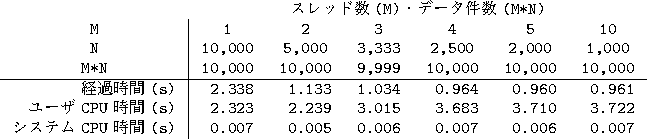
\includegraphics[scale=1.0]{Tbl/threadTimeTbl.pdf}
\end{mytable}

\begin{myfig}{btp}{スレッド数による実行時間の変化}{threadTimeGrph}
  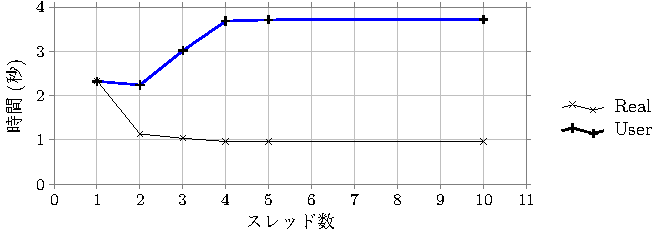
\includegraphics[scale=1.0]{Tbl/threadTimeGrph.pdf}
\end{myfig}

スレッド数が1の時は,経過時間(Real)とユーザCPU時間(User)が,
ほぼ,同じになる.
一つのコア\footnote{従来のCPUのこと.}が全力で合計を計算した結果である.

スレッド数が1〜6の間は,経過時間がスレッド数に反比例して短くなる.
合計の計算時間に対応するユーザCPU時間は,ほぼ一定である.
使用したコンピュータが持つ六つのコアが,
最大で六つのスレッドに割当てられ,
真に並列実行された結果である.

スレッドの数が6〜10に増加する間,経過時間は,ほぼ一定である.
しかしユーザCPU時間が増加している.
必要な計算量は一定なのに長いCPU時間を必要とするので,
コアの性能が悪化したように見える.

コアの性能が悪くなったように見えるのは,
ハイパースレッディング・テクノロジー\cite{hyperThreading}により,
コアの数が倍(12個)あるように見せかけているためである.
ハイパースレッディング・テクノロジーは,
単一スレッドを実行する場合は遊んでしまうコア内のユニットを,
二つのスレッドを同時に実行することで効率よく使用する技術である.
見かけ上コアの数が二倍になるが,合計の性能は二倍には達しないので,
コアあたりの性能が下がったように見える.
%\footnote{
%この計測結果からは,
%ハイパースレッディング・テクノロジーは,
%性能の改善に余り寄与していないように見える.
%}

%スレッド数を12以上にすると,
%(見かけ上の)コア全てが常時使用されるので,
%経過時間,ユーザ時間の合計のどちらも一定になる.

%==============================================================================
\section{CPU仮想化の実装例}
第\ref{tacosVirtualCPU}章にTacOSのCPU仮想化の例を示す.
この例は,{\cmml}で記述したカーネル内データ構造や,
プロセス切換えプログラム,プロセススケジューラ等の実装を含む.
また,プロセスのメモリ配置についても説明している.

%==============================================================================
\section{まとめ}
本章では,時分割多重によるCPUの仮想化について学んだ.
プロセスは幾つかの状態を持ち,
実行できない状態の場合はCPUを割当てない.
プロセスはイベントやタイムスライシングにより状態が変化する.
CPUは,実行を中断するプロセスから次に実行するプロセスに,
コンテキストスイッチを行う.

PCBはプロセスを表現するカーネル内の重要なデータ構造である.
例えばプロセスの待ち行列はPCBの待ち行列として表現されるし,
プロセスの実行が中断する時はPCBにコンテキストが保存される.

スレッドを導入することで,
SMPに対応したプロセスのモデルを表現できる.
スレッドにはカーネルスレッドとユーザスレッドがあった.
また,これらを組み合わせた三つのスレッドモデルがあった.
POSIXスレッドを用いてデータの合計を計算する処理を高速化する
プログラム例を紹介し,実行時間の計測結果を示した.
スレッド数がCPU(コア)数以内の場合は,
スレッド数に反比例して実行時間が短くなることが確認できた.

%==============================================================================
\section*{練習問題}
\begin{enumerate}
  \renewcommand{\labelenumi}{\ttfamily\arabic{chapter}.\arabic{enumi}}
  \setlength{\leftskip}{1em}
\item 次の言葉の意味を説明しなさい.
  \begin{enumerate}
    \item 時分割多重
    \item コンテキストスイッチ
    \item Dispatch(ディスパッチ)
    \item Preemption(プリエンプション)
    \item プロセスの状態
    \item プロセスの状態遷移
    \item RETI命令
    \item PCB
    \item 待ち行列
    \item 実行可能列
    \item スレッド
    \item カーネルスレッド
    \item ユーザスレッド
    \item One-to-One Model
    \item Many-to-One Model
    \item Many-to-Many Model
  \end{enumerate}
\item POSIXスレッドについて調査しなさい.
\end{enumerate}
 % CPUの仮想化
\chapter{CPUスケジューリング}
プロセス(スレッド)の実行順序を決めることをスケジューリングと呼ぶ\footnote{
プロセスとスレッドの両方にあてはまることが多いので,
この章ではプロセスのスケジューリングを前提に議論する.}.
システム内で最も貴重な資源であるCPUの割当てを決める重要な機能である.

\section{評価基準}
スケジューリングの良し悪しを判断する評価基準には次のようなものがある.

\begin{description}
\item[スループット(Throughput)]
単位時間あたりに処理できるジョブ数のことである.
大きい方が良い.

\item[ターンアラウンド時間(Turnaround time)]
プロセスが実行できるようになってから終了するまでの時間のことである.
短いほうが良い.
バッチ処理で,
ユーザがジョブを提出してから実行結果の印刷物が届くまでの時間を
イメージすると分かりやすい.

\item[レスポンス時間(Response time)]
対話的なシステム(TSSやデスクトップパソコン)において,
ユーザが操作した影響で出力が変化し始めるまでの時間である.
例えば,エンターキーを入力したあと画面が変化を始めるまでの時間である.
対話的なアプリケーションの操作性に大いに影響がある.
当然,短いほうが良い.

\item[締め切り(Deadline)]
制御用に用いられる{\bf リアルタイムシステム(Real-time system)}では,
決められた時刻(締め切り)までに結果を出すことが求められる.
必ず時間を守らなければならない場合を
{\bf ハードリアルタイム(Hard real time)},
できる限り時間を守らなければならない場合を
{\bf ソフトリアルタイム(Soft real time)}と呼ぶ.
オペレーティングシステムは,
制御用プロセスが締め切りを守ることができるスケジューリングを行う必要がある.

\item[その他]
システムの使用方法などにより様々な評価基準が考えられる.
例えば,
モバイルデバイスではバッテリーために{\bf 省エネルギー}が評価基準になり得る.
\end{description}

\section{システムごとの目標}
システムの種類によって,
スケジューリングの目標は異なる.
\tabref{schedulingObjective}に概略をまとめる.

\begin{itemize}
\item メインフレームでバッチ処理を行う場合は,
ユーザとの対話的な処理ではないので,
{\bf スループット}を優先する.
例えば,コンテキストスイッチにも処理時間が必要なので,
プリエンプションを行わないスケジューリング方式を採用し,
コンテキストスイッチの回数を少なくすること等が考えられる.
また,ユーザが結果を早く受取ることができるように,
{\bf ターンアラウンド時間}にも気を使う必要がある.

\item ネットワークサーバはネットワークに接続され,
複数のクライアントから同時に多数の要求を受付けて処理する.
この場合は,
クライアントを操作しているユーザの操作性を損なわない{\bf レスポンス時間}と,
多数の要求を処理するための{\bf スループット}が両立することが望まれる.
両者のバランスが良いスケジューリングが求められる.

\item デスクトップパソコンは一人のユーザが独占して使用するコンピュータである.
ユーザは,複数の処理を同時にすることは少ない.
ユーザの操作に素早く反応するために{\bf レスポンス時間}が重要である.
例えば,ユーザがワードプロセッサを操作している間に
バックグラウンドでメールの着信チェックを行うプロセスが動く場合,
ワードプロセッサが軽快に動くことを重視し,
メールの着信チェックプロセスの性能が落ちても構わない.
ユーザが直接操作するプロセスを優先するスケジューリングが求められる.

\item ノートパソコンやスマートフォンのようなモバイルデバイスでは,
基本的にはデスクトップパソコンと同じように{\bf レスポンス時間}が重視される.
しかし,バッテリーで駆動される場合は
消費電力が少なくなるような工夫も必要である.
例えば,プロセスの切換え頻度を少なくすることで,
エネルギーの消費を小さくするスケジューリングを採用することが考えられる.

\item 組込み制御用のコンピュータの場合,
{\bf 締め切り}までに処理を完了することが重要である.
例えば,時速50kmで走行するエレベータ\footnote{
高層ビルのエレベータの中にはもっと高速なものもある.
}の制御コンピュータが,
1秒遅刻してブレーキを掛けたらどうなるだろうか.
時速50kmは秒速13mなので,エレベータは13m行き過ぎて停まることになる.
最上階,または,最下階を目指しているとき13m行き過ぎると
エレベータは天井か床に激突してしまう.
エレベータのブレーキ制御プロセスは{\bf ハードリアルタイム}に分類できる.
同じエレベータでも,
現在階数の表示はタイミングが少し遅れても大きな影響はない.
エレベータの階数表示プロセスは{\bf ソフトリアルタイム}に分類できる.
\end{itemize}

\begin{mytable}{btp}{スケジューリングの目標}{schedulingObjective}
  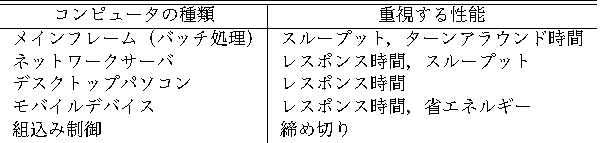
\includegraphics[scale=1.0]{Tbl/schedulingObjective.pdf}
\end{mytable}

\section{プロセスの振舞}
一般に,プロセスは計算と入出力を繰り返す.
計算と入出力にかかる時間の割合に応じて,
二種類のプロセスに分類できる.

\subsection{CPUバウンドプロセス}
例として,動画を圧縮するビデオエンコーディング・プロセスを考えてみよう.
プロセスは,\figref{cpuIoBound}(a)に示すように,次の三つの処理を繰り返す.

\begin{enumerate}
\item 未圧縮の動画ファイルを少し読む.
\item 圧縮処理を行う.
\item 結果を圧縮済み動画ファイル書込む.
\end{enumerate}

ビデオエンコーディング・プロセスはCPUが行う圧縮処理に長い時間がかかり,
入出力にかかる時間が短い.
このようにCPU処理にかかる時間が相対的に長いプロセスのことを
{\bf CPUバウンド(CPU-bound)プロセス}と呼ぶ.
また,CPUが使用される期間を{\bf CPUバースト(CPU burst)},
I/Oが使用される期間を{\bf I/Oバースト(I/O burst)}と呼ぶ.
CPUバウンドプロセスは長いCPUバーストと短いI/Oバーストを持つ.

\begin{myfig}{btp}{CPUバウンドとI/Oバウンドプロセス}{cpuIoBound}
\myincludegraphics{cpuBound-crop.pdf}{scale=0.66}
%~~~~

\vspace{0.8cm}

\myincludegraphics{ioBound-crop.pdf}{scale=0.66}
\end{myfig}

\subsection{I/Oバウンドプロセス}
二つ目の例としてスプレッドシート・プロセスを考えてみよう.
スプレッドシート・プロセスは,
まず,ユーザが何れかのセルにデータを入力するのを待つ.
次に,入力されたデータを用いてスプレッドシートの再計算を行い結果を表示する.
ユーザがセルにデータを入力するたびに同様な処理を繰り返す.
このプロセスは\figref{cpuIoBound}(b)に示すように,
ユーザ操作を待つ長い入力待ちと,
再計算と表示を行う短いCPU処理を行う.
このような,長いI/Oバーストと短いCPUバーストを持つプロセスを
{\bf I/Oバウンド(I/O-bound)プロセス}と呼ぶ.

\section{スケジューリング方式}
いくつかの代表的なスケジューリング方式を紹介する.

\subsection{First-Come, First-Served(FCFS)スケジューリング}
Ready状態になった順(到着順)に実行する方式である.
Running状態になったらブロックするまで実行を継続する.
プリエンプションはしない.
以下の例ではCPUバースト一回分の期間しか示さないが,
実際は,\figref{cpuIoBound}に示すようにCPUバースが繰り返し発生する.

FCFS方式は実行可能列をFIFOにするだけで実現できるが性能は良くない.
例えば次の三つのプロセスが時刻0で,
$P_1$,$P_2$,$P_3$の順にReady状態になったとする.

\begin{center}
\begin{tabular}{c c c}
プロセス & 到着時刻 & CPUバースト時間(ms) \\
\hline
$P_1$    & 0 & 100 \\
$P_2$    & 0 & 20 \\
$P_3$    & 0 & 10 \\
\end{tabular}
\end{center}

この時,三つのプロセスの実行開始・終了の時刻を図で表すと次のようになる.

\begin{center}
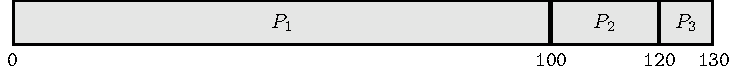
\includegraphics[scale=1.0]{GanntChart/fcfs1.pdf}
\end{center}

平均ターンアラウンド時間を計算すると,
$(100+120+130) / 3 = 117$ ms となる.
もしも,プロセスの到着順が$P_2$,$P_3$,$P_1$の順だったとすると,
三つのプロセスの実行開始・終了の時刻は図のようになる.

\begin{center}
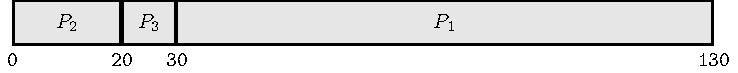
\includegraphics[scale=1.0]{GanntChart/fcfs2.pdf}
\end{center}

この場合の
平均ターンアラウンド時間を計算すると,
$(20+30+130) / 3 = 60$ ms となる.
このように,FCFSでは最悪な平均ターンアラウンド時間を選択することもある.
プリエンプションをしないので,
一旦,CPUバウンドなプロセスが実行を開始すると,
他のプロセスは長い時間待たされる.

\subsection{Shortest-Job-First(SJF)スケジューリング}
SJF方式\footnote{皆さんの教科書ではSPTのこと.}は,
平均ターンアラウンド時間を最小にするスケジューリング方式である.
SJF方式ではCPUバースト時間が短いものを先に実行するようにスケジューリングする.
実行可能列はCPUバースト時間が短い順にソートされている.

三つのプロセスがあった時,
実行順に各プロセスの実行時間が$T_1$,$T_2$,$T_3$とすると,
平均ターンアラウンド時間は,
$(T_1+(T_1+T_2)+(T_1+T_2+T_3))/3=T_1+T_2*2/3+T_1/3$となるり,
先に実行したプロセスの実行時間ほど結果に及ぼす影響が大きいことが分かる.
実行時間が短いプロセスを先に実行するスケジューリング方式は,
平均ターンアラウンド時間を最小にする.

前出の三つのプロセスをSJF方式でスケジューリングした時の,
実行開始・終了時刻は次の図のようになる.

\begin{center}
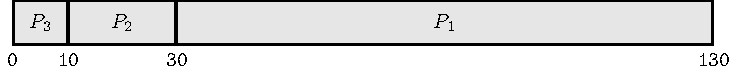
\includegraphics[scale=1.0]{GanntChart/sjf1.pdf}
\end{center}

この図より平均ターンアラウンド時間を求めると
$(10+30+130)/3 = 57$ ms となり,これまでで最短である.
しかし,次回のCPUバースト時間を知ることは一般には不可能なので,
SJF方式は現実的な方式ではない.
次回のCPUバースト時間を予測することで擬似的なSJF方式を実現する.

次回のCPUバースト時間を予測する方法として,
指数平滑平均(exponential average)を用いる例を紹介する.
次回の予測時間を$T_{n+1}$,
前回の予測時間を$T_{n}$,
前回の実際のCPUバースト時間を$t_{n}$とすると,
$0 \le \alpha \le 1$の時,
指数平滑平均は次の式で表すことができる.

\[T_{n+1} = \alpha t_n + ( 1 - \alpha ) T_n\]

この式から

\[T_{n+1} = \alpha t_n + ( 1 - \alpha ) \alpha t_{n-1} + \dots +
 ( 1 - \alpha )^j \alpha t_{n-j} + \dots + (1 - \alpha )^{n+1} T_0 \]

を得る.$\alpha = 0.5$ の場合は,

\[T_{n+1} = 0.5 t_n + 0.5^2 t_{n-1} + \dots +
0.5^{j+1} t_{n-j} + \dots + 0.5^{n+1} T_0 \]

となる.
この式は,過去のCPUバースト時間を,
最近のものほど大きな重みを付けて平均したものになっている.
つまり,次回のCPUバースト時間は,
過去のCPUバースト時間と同程度であろうとの仮定に基づいた予測値を計算している.

\subsection{Shortest-Remaining-Time-First(SRTF)スケジューリング}
SRTF方式\footnote{皆さんの教科書ではSRPTのこと.}は,
プリエンプション付きのSJF方式である.
プロセスがReady状態になるとき,
このプロセスのCPUバースト時間と
実行中のプロセスの{\bf 残りCPUバースト時間}とを比較し,
{\bf 残りCPUバースト時間}の方が長いときプリエンプションをおこす.
次の例でSJTとSRFTを比較してみよう.

\begin{center}
\begin{tabular}{c c c}
プロセス & 到着時刻 & CPUバースト時間(ms) \\
\hline
$P_1$    & 0  & 60 \\
$P_2$    & 10 & 40 \\
$P_3$    & 60 & 30 \\
\end{tabular}
\end{center}

三つのプロセスをSJFでスケジューリングした場合は次の図のようになる.

\begin{center}
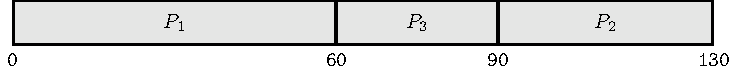
\includegraphics[scale=1.0]{GanntChart/sjf2.pdf}
\end{center}

平均ターンアラウンド時間を計算すると,
$((60-0)+(90-10)+(130-60))/3=70$ ms となる.
三つのプロセスをSRTFでスケジューリングした場合は次の図のようになる.

\begin{center}
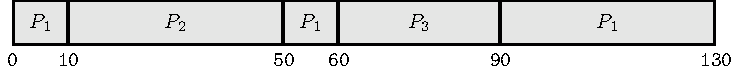
\includegraphics[scale=1.0]{GanntChart/srtf1.pdf}
\end{center}

$P_2$が到着した時,
$P_2$のCPUバースト時間($40$ ms)の方が
$P_1$の残りCPUバースト時間($60 - 10 = 50$ ms)より短いので,
$P_1$はプリエンプションし$P_2$が先に実行される.
$P_3$が到着した時も同様である.
平均ターンアラウンド時間を計算すると,
$((130-0)+(50-10)+(90-60))/3=67$ ms となり,
SJFよりも改善されている.

\subsection{Round-Robin(RR)スケジューリング}
{\bf タイムシェアリングシステム(TSS)}で使用された方式である.
{\bf クォンタム時間(time quantum)},または,
{\bf タイムスライス(time slice)}と呼ばれる10 ms 〜 100 ms 程度の
一定の時間が予め決められている.
実行可能列はFIFOになっている.
実行可能列の先頭のプロセスにCPUが割り付けられてRunning状態になる.
プロセスの実行が{\bf クォンタム時間}連続するとプリエンプションが発生し,
プロセスは実行可能列の最後尾に付け加えられる.

{\bf クォンタム時間($q$)}が短いと{\bf レスポンス時間}が短くなり,
対話的な処理が円滑に行える.
例えば,10個のプロセスがCPUを奪い合うような状況でも,
$q = 10$ ms なら$100$ ms に一度は全てのプロセスにCPUが割り付けられる.
しかし,$q$ を小さくしすぎるとコンテキストスイッチの回数が多くなり,
オーバーヘッドが大きくなる.
逆に $q$ が長いとFCFSと同じ結果になる.

前出の三つのプロセスをRR方式($q = 10$ ms)でスケジューリングした例を
次の図に示す.
なお,
新規プロセスと,
クォンタム時間を使い切りプリエンプションしたプロセスが,
同時に実行可能列に追加される場合は,
新規プロセスを優先することにする.

\begin{center}
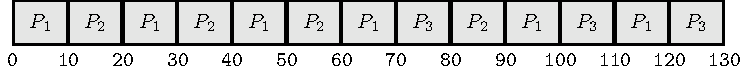
\includegraphics[scale=1.0]{GanntChart/rr1.pdf}
\end{center}

平均ターンアラウンド時間を計算すると,
$((120-0)+(90-10)+(130-60))/3=90$ ms となる.
次に $q = 50$ ms でスケジューリングした例を示す.

\begin{center}
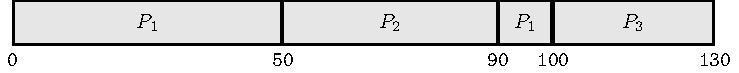
\includegraphics[scale=1.0]{GanntChart/rr2.pdf}
\end{center}

平均ターンアラウンド時間を計算すると,
$((100-0)+(90-10)+(130-60))/3=83$ ms となる.
$q = 50$ ms でスケジューリングした方が,
平均ターンアラウンド時間が短くなった上に,
コンテキストスイッチの回数が少ない.
このようなプロセスの集合に対しては,
$q = 10$ ms はクォンタム時間が短すぎると言える.

\subsection{Priority (優先度順)スケジューリング}
プロセス毎に決められた{\bf 優先度}を基に行うスケジューリング方式である.
実行中に優先度が変化する{\bf 動的優先度}を用いる方法と,
プロセス生成時に決められ変化しない{\bf 静的優先度}を用いる方法がある.
TacOSは{\bf 静的優先度}を用いる優先度順スケジューリング方式を用いる.
SRTF方式は,
次回CPUバースト時間が短い順の{\bf 動的優先度}方式と考えられる.

優先度順スケジューリング方式の問題点は,
優先度の低いプロセスが全く実行されない{\bf スタベーション(stavation)}が
発生することである.
これの対策として,
実行可能列に留まるプロセスの優先度を徐々に高くしていく
{\bf エージング(aging)}が用いられる.
実行可能列に長く留まるプロセスは優先度が高くなり,
やがて実行される.

\subsection{Multilevel Feedback Queue(FB)スケジューリング}
Windows,macOS,UNIX等で広く使用されているスケジューリング方式である.
\figref{multilevelFeedbackQueue}に示すように実行可能列を優先度別に複数設ける.
優先度が近いプロセスが同じ実行可能列に登録される.
同じ実行可能列ではRR方式でスケジューリングするので\footnote{
実行可能列ごとに,異なるスケジューリング方式を採用することも可能である.
},
列内でプロセスの順番は優先度とは関係がない.
CPUを割り付ける際は,
優先度の高い実行可能列から順に調べ,
最初に見つかった空ではない実行可能列を使用する.

\myfigure{btp}{scale=0.6}{multilevelFeedbackQueue-crop.pdf}
{Multilevel Feedback Queue}{multilevelFeedbackQueue}

プロセスの優先度は動的に変化する方式を用いる.
CPUバウンドなプロセスの優先度は急激に引き下げられ,
プロセスは下位の実行可能列に移動する.
長く実行可能列に留まっているプロセスは{\bf エージング}により
優先度が引き上げられ,上位の実行可能列に移動する.
実行中のプロセスより上位の実行可能列にプロセスが登録されると
プリエンプションが発生し,実行中のプロセスはCPUを取り上げられる.

\section{TacOSのスケジューラ}
実行可能になったプロセスをスケジューリングするプログラムを{\bf スケジューラ}と呼ぶ.
スケジューラの例として,
TacOSのスケジューラのソースプログラムを\figref{tacosSch}に示す\footnote{
\figref{tacosSch}はTacOSのソースコード
\url{https://github.com/tctsigemura/TacOS/blob/master/os/kernel/kernel.cmm}
の一部である.}.
TacOSの実行可能列は,
PCBの番兵付き重連結環状リストとして表現する
(\figref{tacosReadyQueue}参照).

\begin{figure}[btp]
\lstinputlisting{Lst/sch.cmm}
\caption{TacOSのスケジューラ・ソースプログラム}
\label{fig:tacosSch}
\end{figure}

\begin{description}
\item[1〜7行] 関数\|insProc()|は,
実行可能列にPCBを登録するために使用される.
スケジューラ以外からも呼出される汎用的なものである.

\item[9〜19行] 関数\|schProc()|がスケジューラである.
\|enice|がプロセスの優先度である.
\|enice|は値が小さい方が優先度が高い.
スケジューラは,
実行可能列(\|readyQueue|)を番兵PCBの次のPCBから開始して(14行),
挿入するプロセスの\|enice|より大きいものを探す(15,16行).
大きいものを見つけたら\|insProc()|を使用して,
見つけたPCBの直前に新しいプロセスのPCBを挿入する(17行).
実行可能列の最後には,常時IdleプロセスのPCBが置かれている
(\figref{tacosReadyQueue}参照).
Idleの\|enice|は最大値に設定されているので15行のループは必ず正常に終了する.

現在の実装では,\|enice|はプロセス生成時に\|nice|と同じ値に設定され,
その後は変化しない.
TacOSは{\bf 静的優先度}を用いる{\bf 優先度順スケジューリング方式}を用いていることになる.
将来,\|enice|の値を動的に変化させるように変更すれば,
{\bf 動的優先度}方式になる.

\|setPri()|関数はPSWの割込み許可フラグを操作するために使用している.
詳しくは「\ref{setPri} setPri()関数」で説明する.
\end{description}
 % スケジューリング
\chapter{プロセス同期}
\label{synchronaization}
これまで見てきたように,
複数のプロセス(スレッド)が並行して実行される.
複数の並行して実行されるプロセス(スレッド)が,決して競合することなく,
必要に応じて協調して動作するために,プロセス(スレッド)間で同期をとる必要がある.
この章ではプロセス(スレッド)間の同期について勉強する.

\section{競合(Race Condition, Competition)}
複数のプロセス(スレッド)が資源を共有して処理を進めることがある.
ここで言う資源とは
「スレッド間で共有する変数」,
「プロセス間で共有するメモリ」,
「カーネル内部のデータ構造」,
「ファイル」,
「入出力装置」
等が考えられる.
共有する資源をプロセス(スレッド)がアクセスする時,
きちんとした取り決めが無いと誤った結果になる場合がある.

例えば,銀行口座を管理する架空の例を考えよう.
一つのプロセス内で,
入金を処理するスレッドと,
引き落としを処理するスレッドが並行して実行されているとする.
\figref{race}にこのプロセスの処理内容の一部をTeC風のアセンブリ言語で示す.

\begin{myfig}{btp}{共有変数をアクセスする二つのスレッド}{race}
\lstinputlisting[numbers=none]{Lst/race.txt}
\end{myfig}

ほぼ同時に,プロセスが給料3万円の振込と,カード料金2万円の引き落としを受信した場合を考えてみよう.
二つのスレッドが競って\|account|変数の更新をすることになる.
処理前は\|account|変数に口座の残高10万円が記録されていたとする.

\begin{quote}
\begin{enumerate}
\item (1)→(2)→(3)→(a)→(b)→(c)の順で実行された場合 \\
\|account|変数の値は11万円になり正しい結果になる.

\item (a)→(b)→(c)→(1)→(2)→(3)の順で実行された場合 \\
\|account|変数の値は11万円になり正しい結果になる.

\item (1)→(2)→(a)→(b)→(c)→(3)の順で実行された場合 \\
入金管理スレッドが途中でpreemptionし,
引き落としスレッドが実行された後,
入金管理スレッドが再開された場合である.
\|account|変数の値は13万円になる.

\item (1)→(a)→(2)→(b)→(3)→(c)の順で実行された場合 \\
二つのCPUが並列にスレッドを実行した場合である.
\|account|変数の値は8万円になる.
\end{enumerate}
\end{quote}

以上のように,
スレッドの実行順序等により計算結果が間違ってしまうことがある.
これは資源の利用について,
{\tt 競合(Race Condition または Competition)}が発生しているからである.

\section{クリティカルセクション(Critical Section)}
\label{criticalsection}
競合が発生するのは,
一方のスレッドが自分のCPUレジスタにコピーした\|account|の値を
変更し書き戻すまでの間(変更中)に,
もう一方のスレッドが\|account|の値を
自分のCPUレジスタにコピーすることが原因である.
「変更中」の共有変数に他のスレッドがアクセスすることを禁止する必要がある.
他のスレッドが共有変数にアクセスすることが許されないプログラムの区間を
{\tt クリティカルセクション(Critical Section)},または,
{\tt クリティカルリージョン(Critical Region)}と呼ぶ.

\figref{race}の例で「(1)から(3)」と「(a)から(c)」は
\|account|変数のクリティカルセクションであり,
この区間をどれかのスレッドが実行している間は,
他のスレッドが\|account|変数にアクセスしてはならない.
クリティカルセクションの競合問題を効率よく解決するためには,
次の三つの条件を満たす必要がある.

\begin{quote}
\begin{enumerate}
\item 二つ以上のプロセス(スレッド)が同時にクリティカルセクションに入らない.
\item クリティカルセクションに入っているプロセス(スレッド)がない時は,
待たされることなくクリティカルセクションに入ることができる.
\item クリティカルセクションに入るために永遠に待たされることがない.
\end{enumerate}
\end{quote}

\section{相互排除(Mutual Exclusion)}
複数のプロセス(スレッド)が同時にクリティカルセクションに
入らないように制御することである.
{\bf 排他制御}または{\bf 相互排他}とも呼ばれる.
{\bf 相互排除}を達成するために,
プロセス(スレッド)は,
クリティカルセクションに入る際に権利を得る手続きを行う.
これを行うプログラムの部分を
{\bf エントリーセクション(Entry Section)}と呼ぶ.
クリティカルセクションを出る際に権利を返却する手続きを行う.
これを行うプログラムの部分を
{\bf エグジットセクション(Exit Section)}と呼ぶ.

\subsection{割込み禁止}
\label{disableInterrupt}
シングルプロセッサ(CPUが一つしかない)システムでは,
クリティカルセクションを実行するとき割込みを禁止することで目的を達成できる.
\figref{disableInterrupt}に\figref{race}を改良したプログラムを示す.

\begin{myfig}{btp}{割込み禁止による相互排除}{disableInterrupt}
\lstinputlisting[numbers=none]{Lst/disableInterrupt.txt}
\end{myfig}

エントリーセクションで
DI(Disable Interrrupt)命令を実行し割込みを禁止する.
エグジットセクションで
EI(Enable Interrrupt)命令を実行し割込みを許可する.
クリティカルセクションでは,
CPUが割込みを受付けない\footnote{
再度,割込みが許可されるまで保留になる.
プリエンプションはクリティカルセクションを出るまで遅延する.
}のでプリエンプションは発生しない.
クリティカルセクションの終わりまでCPUは連続して命令を実行する.
また,CPUが一つしかないので他のCPUが\|account|変数をアクセスこともない.
よって,\|account|変数の変更中に他のプロセス(スレッド)が
\|account|変数をアクセスすることはない.

この方法は簡単に相互排除を行うことができるが,
割込み禁止時間が長くならないように注意する必要がある.
割込み禁止が長くなると,
タイマーからの割込みを取りこぼし時計が正確に進まなくなったり,
入出力装置の制御が間に合わなくなるなどの弊害が生じる\footnote{
割込み禁止期間に同じ割込みが複数回発生した場合,
割込み許可になったとき割込みの種類につき一度だけ割込みが発生する.
ハードウェアに,保留になった割込みのカウンタはない.}.
また,DI命令,EI命令は特権命令なので,
カーネル内だけで使用できる手法である.

\subsection{専用命令を用いる方式}
マルチプロセッサ(CPUが複数ある)システムでは,
割込み禁止による方法では目的を達成することができない.
クリティカルセクションでプリエンプションが発生しなくても,
他のCPUによって実行されるプロセス(スレッド)がクリティカルセクションに
入る可能性があるからである.

マルチプロセッサシステムとは,
\figref{hardBlock}に示したメモリを共有するSMPシステムのことである.
複数のCPUによるメモリのアクセスはハードウェアにより順序付けされる.
同じメモリアドレスへのアクセスが競合し,
どちらのCPUが書き込んだ値とも異なる値になることはない.
順序付けの結果,後になった書き込みの結果がメモリに残る.
また機械語命令は,一部の例外を除いて,
途中で割込まれることはない.
このようなシステムでは,
以下の機械語命令を相互排除の目的に使用できる.

\begin{itemize}
\item {\bf TS(Test and Set)命令} \\
TS命令は「(1) メモリの値をCPUレジスタにロード」し,
「(2) 1を同じメモリアドレスに書き込む」命令である.
この二つを他のCPUのメモリアクセスに割込まれることなく,
{\bf アトミック(atomic)}に実行する.
TS命令(\|TS R,M|)の動作は,例えば次のようになる.

\begin{quote}
\begin{enumerate}
\item バスをロックする
\item $R \leftarrow [M]$
\item {\tt if (R==0) } $Zero \leftarrow 1;$ {\tt ~else} $Zero \leftarrow 0;$
\item $[M] \leftarrow 1$
\item バスのロックを解除する
\end{enumerate}
\end{quote}

TS命令は,他のCPUがメモリをアクセスしないように,まずバスをロックする.
次に,メモリの指定番地から値をCPUレジスタにロードする.
また,レジスタの値によってCPUの$Zero$フラグの値を決める.
更に,メモリの指定番地に「1」をストアする.
最後にバスのロックを解除する.
ロードとストアで合計二回のメモリアクセスがあるが,
バスがロックされているので,
TS命令の実行途中に他のCPUがメモリをアクセスすることはない.
\figref{testAndSet}にTS命令の使用例を示す.
JZ命令は$Zero$フラグが「1」の場合のみジャンプする.
この例のように,
クリティカルセクションに入れるようになるまでループで待つ方式を
{\bf ビジーウェイティング(Busy Waiting)}と呼ぶ.

\begin{myfig}{btp}{TS命令の使用例}{testAndSet}
\lstinputlisting[numbers=none]{Lst/testAndSet.s}
\end{myfig}

メモリのクリアは通常のST命令でできる\footnote{
通常の命令もメモリアクセスする度にバスをロックしている.}.
TS命令を用いる場合もクリティカルセクションは割込み禁止で実行する必要がある.
クリティカルセクションでのプリエンプションを避けるためである.
もしも,優先度の低いプロセス(スレッド)が
クリティカルセクション内でプリエンプションすると,
優先度の高いプロセス(スレッド)が
エントリーセクションで{\bf ビジーウェイティング}を始め
{\bf デッドロック}に陥る可能性があるからである.
%「0」をロードしたプロセス(スレッド)は,
%クリティカルセクションでプリエンプションしてはならない.
この方式も,
特権命令DI,EIを使用するのでカーネル内でしか利用できない.

\item {\bf SW(Swap)命令} \\
SW(Swap)命令もSMPシステムでの相互排除に使用できる.
「SW  R, M」は以下を{\bf アトミック(atomic)}に実行する.

\begin{quote}
\begin{enumerate}
\item バスをロックする
\item $T \leftarrow [M]$
\item $[M] \leftarrow R$
\item $R \leftarrow T$
\item バスのロックを解除する
\end{enumerate}
\end{quote}

ここで $T$ はCPU内部の一時的なレジスタ
($T$ レジスタの存在はプログラムから見えない)である.
\figref{swap}にSW命令の使用例を示す.
使用例はTS命令のものと似ているので解説は省略する.

\begin{myfig}{btp}{SW命令の使用例}{swap}
\lstinputlisting[numbers=none]{Lst/swap.s}
\end{myfig}

\item {\bf CAS(Compare And Swap)命令}\\
CAS(Compare And Swap)命令もSMPシステムでの相互排除に使用できる.
例えば「CAS  R0, R1, M」は,以下を{\bf アトミック(atomic)}に実行する.

\begin{quote}
\begin{enumerate}
\item バスをロックする
\item $T \leftarrow [M]$
\item {\tt if ($T==R0$) \{} $[M] \leftarrow R1;~ Zero \leftarrow 1;$
      {\tt \} else \{} $R0 \leftarrow T;~  Zero \leftarrow 0;$ {\tt \}}
\item バスのロックを解除する
\end{enumerate}
\end{quote}

CAS命令を用いたエントリーセクション,
エグジットセクションの作り方も,
TS命令と同様なのでここでは使用例を省略する.
CAS命令を用いると共有資源にロックを掛けない,
{\bf ロックフリー(Lock-free)}なアルゴリズムを実現できる.
前出の銀行口座を管理する架空のプロセス(\figref{race})を
CAS命令を用いて書換えた例を\figref{cas}に示す.

\begin{myfig}{btp}{CAS命令を用いた口座管理プログラムの例}{cas}
\lstinputlisting[numbers=none]{Lst/cas.txt}
\end{myfig}

処理開始時の\|account|の値をG1に保存しておく.
計算結果を格納する際に,
処理開始から\|account|の値が変化していないことを確認してから書き込む.
以前の例では,
他のプロセスが共有資源にアクセスしないように,
何らかのロックを掛けていた.
この方式はロックを掛けずに「結果を書き込む時点で判断」している.
\end{itemize}

\subsection{フラグを用いる方式}
アルゴリズムを工夫しソフトウェアだけで相互排他を実現する方式である.
中でも1981年にG. L. Peterson が発表した
{\bf Petersonのアルゴリズム(Peterson's solution)}が有名なので紹介する.
\figref{peterson}にJava風の言語で書いた例を示す.

\begin{myfig}{btp}{Petersonのアルゴリズム}{peterson}
\lstinputlisting[numbers=none]{Lst/peterson.txt}
\end{myfig}

このアルゴリズムの特徴は次の通りである.

\begin{quote}
\begin{enumerate}
\item マルチプロセッサシステムでも使用できる.
\item 2プロセス(スレッド)以上に拡張可能だが複雑になる.
\item 最近のプロセッサと相性が悪い.(out-of-order実行)
\end{enumerate}
\end{quote}

\section{セマフォ(Semaphore)}
これまでに紹介してきた相互排除は,
主に{\bf ビジーウェイティング}を用いるものであり,
待っている間もCPUを使用し続ける.
また、割込み禁止にする必要があるのでカーネル内でしか使用できない.
これらは、カーネル内で短時間で終わる相互排除のために適しているが,
長時間に渡る場合やユーザプログラムが直接使用する場合には適さない.

そこで,オペレーティングシステムが提供するより洗練された
プロセス同期機構である{\bf セマフォ}を紹介する.
なお,これまでに紹介してきた相互排除は,セマフォを実現するためにも使用される.

\subsection{概要}
{\bf セマフォ(Semaphore:腕木式信号機)}は,
1965年に E. W. Dijkstra が提案したデータ型\footnote{
C言語なら構造体を用いてセマフォ型を宣言する.
{\tt typedef struct \{ ... \} Semaphore;}
}である.
語源となった腕木式信号機は,
鉄道で使用される\figref{semaphore}のような信号機である.

\myfigure{btp}{scale=0.4}{Fig/semaphore-crop.pdf}{腕木式信号機}{semaphore}

セマフォ型の変数は内部にカウンタ\footnote{
腕木信号機の進行・停止のように二つの状態しか取らないものを
{\bf バイナリセマフォと}呼ぶ.
ここで取り上げるカウンタを持つものは{\bf カウンティングセマフォ}と呼ぶ.
カウンタの値は0以上の整数値である.
}を持ち,また,プロセスの待ち行列を作ることができる.
セマフォ型(\|Sempahore|)の変数には,
{\bf P操作({\it Proberen}:try)}と{\bf V操作({\it Verhogen}:raise)}を
行うことができる.
カーネルはP操作とV操作を,
ユーザプロセスにシステムコールとして提供したり,
カーネル内部のサービスモジュールやデバイスドライバにサブルーチンとして提供したりする.
セマフォはプロセス(スレッド)の状態を{\bf 待ち(Waiting)状態}に変える.
{\bf ビジーウェイティングでは無い}のでCPUを無駄遣いすることはない.

\begin{quote}
\begin{description}
\item[P操作(P(S))]
%クリティカルセクションのエントリーセクション等で使用できる.
セマフォ(S)の値が1以上ならセマフォの値を1減らす.
値が0ならプロセス(スレッド)を待ち(Waiting)状態にし,
セマフォの待ち行列に追加する.
アルゴリズムをC言語風に記述したものを\figref{semPV}(a)に示す.
\item[V操作(V(S))] %クリティカルセクションのエグジットセクション等で使用できる.
セマフォ(S)の待ち行列にプロセス(スレッド)がある場合は,
それらの一つを起床させる.
待っているプロセス(スレッド)が無い場合は,セマフォ(S)の値を1増やす.
アルゴリズムをC言語風に記述したものを\figref{semPV}(b)に示す.
\end{description}
\end{quote}

\begin{myfig}{btp}{セマフォのアルゴリズム}{semPV}
\small\begin{center}
\begin{minipage}{0.48\columnwidth}
\lstinputlisting[numbers=none]{Lst/semP.c}
\centerline{(a) P操作}
\end{minipage}\hspace{1em}
\begin{minipage}{0.48\columnwidth}
\lstinputlisting[numbers=none]{Lst/semV.c}
\centerline{(b) V操作}
\end{minipage}
\end{center}
\end{myfig}

\subsection{相互排除問題の解}
初期値が1のセマフォを用いて相互排除問題の解を示すことができる.
前出の架空の銀行口座管理プロセスの例を,
セマフォを用いて解決したものを\figref{semMutex}に示す.

\begin{myfig}{btp}{セマフォを用いた相互排除問題の解}{semMutex}
\lstinputlisting{Lst/semMutex.c}
\end{myfig}

1行の\|account|は相互排除が必要なスレッド間の共有変数である.
2行の\|Semaphore|型の変数\|accSem|が排他制御に使用するセマフォである.
\|accSem|は1で初期化される.
クリティカルセクションに入るスレッドは,
まず,6行か14行で\|accSem|にP操作を行う.
どちらか先にやって来たスレッドがP操作を行った時点で\|accSem|の値が0になる.

遅れてやって来たスレッドは\|accSem|の値が0の間はクリティカルセクションに
入ることができない.
先のスレッドがクリティカルセクションを出て
8行か16行で\|accSem|にV操作を行ったら,
後のスレッドがクリティカルセクションに入ることができる.

\subsection{生産者と消費者問題(Producer-Consumer Problem)の解}
生産者プログラム(スレッド)はデータを生産し有限な長さの
{\bf リングバッファ(ring buffer)}に書き込む.
消費者プログラム(スレッド)はリングバッファからデータを読み出し消費する.
この時,満杯のリングバッファに更に書き込んだり,
空のリングバッファらデータを読み出したりしないように,
プログラム(スレッド)間で歩調を合わせる(同期する)必要がある.
セマフォを用いた解を\figref{semProducerConsumer}に示す.

\begin{myfig}{btp}{セマフォを用いた生産者消費者問題の解}{semProducerConsumer}
\lstinputlisting{Lst/semProducerConsumer.c}
\end{myfig}

\begin{quote}
\begin{description}
\item [リングバッファとセマフォ]
1行の\|buffer|は大きさ\|N|のリングバッファである.
型は応用によって決まるので,リングバッファの型は仮に\|Data|型としている.
2行の\|emptySem|はリングバッファの空きスロット数を表すセマフォである.
最初は全てのスロットが空きなので初期値は\|N|である.
3行の\|fullSem|はリングバッファの使用中スロット数を表すセマフォである.
最初は全てのスロットが空きで,
使用中のスロットは無いので,初期値は\|0|にしている.

\item [生産者スレッド]
4行から始まる\|producerThread|が,
データを生産しリングバッファに書き込むスレッドである.
5行の変数\|in|はリングバッファの次回書込み位置を表すローカル変数である.
0,1,2,...,N-1,0,1,2,...の順に値が変化する.
{\bf \|in|はスレッドのローカル変数なので,相互排除をする必要がない.}

\|producerThread|は,
7行でデータを作り,
8行で空きスロット数が1以上なら\|emptySem|の値を減らして,
9行でデータをリングバッファに書き込む.
10行で\|in|の値を更新しているが,
\|in|はローカル変数なので11行より後でも良い.
11行で使用中スロット数\|fullSem|の値を増加させる.

\item [消費者スレッド]
14行から始まる\|consumerThread|は,
データをリングバッファから読み出して消費するスレッドである.
15行の変数\|out|はリングバッファの次回読出し位置を表すローカル変数である.
{\bf \|out|もスレッドのローカル変数なので,相互排除をする必要がない.}

\|consumerThread|は,
17行で空きスロット数が1以上なら\|fullSem|の値を減らして,
18行でデータをリングバッファから読み出す.
19行で\|out|の値を更新する.
20行で空きスロット数\|emptySem|の値を増加させる.
21行で読み出したデータを使用する.
\end{description}
\end{quote}

\subsection{複数生産者と複数消費者問題(Producer-Consumer Problem)の解}
前の問題で,
関数\|producerThread()|,\|consumerThread()|それぞれについて,
複数のスレッドが存在する場合を考える.
バッファに関する同期の他に,
書き込み位置(\|in|),取出し位置(\|out|)に関する排他制御が必要になる.
解を\figref{semMultiProducerConsumer}に示す.

\begin{myfig}{btp}{セマフォを用いた複数生産者・複数消費者問題の解}
{semMultiProducerConsumer}
\lstinputlisting{Lst/semMultiProducerConsumer.c}
\end{myfig}

\begin{quote}
\begin{description}
\item [リングバッファとセマフォ]
1行から3行に変更はない.

\item [生産者スレッド]
次回書き込み位置を表す\|in|変数を複数の\|procucerThread|で共有する必要がある.
\|in|変数の宣言を5行に移動し,スレッド間の共有変数に変更した.
また,\|in|変数を\|procucerThread|間で相互排除するためのセマフォ\|inSem|を
6行に追加した.

\|producerThread|では,\|in|変数の参照や書き換えを行う12行と13行が
\|in|変数に関するクリティカルセクションである.
11行と14行に\|inSem|を用いた相互排除機構を追加した.

\item [消費者スレッド]
次回読み出し位置を表す\|out|変数について,
生産者スレッドと同様な相互排除機構を追加してある.
\end{description}
\end{quote}

\subsection{リーダ・ライタ問題(Readers-Writers Problem)の解}
共有データに対して,
読み出し{\bf だけ}するリーダプロセス(スレッド)と,
読み出し書き込みの両方を行うライタプロセス(スレッド)の
二種類がある場合に,
単に資源をロックするより{\bf 並行性(concurrency)}を高くすることができる.
リーダプロセス(スレッド)は,値を読み出すだけなので,
他のリーダプロセス(スレッド)と同時に共有データをアクセしても良い.
ライタプロセス(スレッド)は,値を書換えるので,
他のライタともリーダとも同時に共有データをアクセスすることは許されない.
セマフォによる解を\figref{semReaderWriter}に示す.

\begin{myfig}{btp}{セマフォを用いたリーダ・ライタ問題の解}{semReaderWriter}
\lstinputlisting{Lst/semReaderWriter.c}
\end{myfig}

\begin{quote}
\begin{description}
\item [共有データとセマフォ]
1行の\|records|が共有データである.
2行の\|rwSem|は共有データの相互排除用のセマフォである.
これらは,全てのスレッドに関係がある.

\item [ライタスレッド]
4行の\|writerThread|は共有データを書き換えることがあるスレッドである.
書き換え途中に他のスレッドが共有データをアクセスすることを禁止するために,
\|writerThread()|は7行で\|rwSem|にロックを掛ける.
9行でロックを解除するまで,
他のライタもリーダも同時に共有データにアクセスすることはできない.
このようなロックを{\bf 排他ロック(exclusive lock)}と呼ぶ.

\item [リーダスレッド]
16行の\|readerThread|は共有資源を読むことだけする.
書き換え途中の不完全なデータを読み出さないように,
\|writerThread|と相互排除を行う必要がある.
しかし,書き換え途中以外なら,
他のリーダスレッドと同時にデータを読んでも構わない.

13行の\|cnt|変数はリーダスレッド間で共有される.
14行の\|cntSem|セマフォは\|cnt|変数の相互排除用である.
リーダスレッドはこれらを使用し,
\|records|共有データを読み出し中のリーダスレッドの数を管理する.
19行と20行,24行と25行の二箇所が,
\|cnt|変数に関するクリティカルセクションである.

19行では最初に読み出しを始めるリーダを判断し,
最初のリーダだけが代表して\|rwSem|にロックを掛ける.
二番目にやって来たリーダはロックを掛けないのでリーダ相互は排他されない.
しかし,排他ロックを用いるライタとは相互排除される.
このようなロックを{\bf 共有ロック(shred lock)}と呼ぶ.
25行で最後に読み出しを終えるリーダを判断し,
最後のリーダだけが代表して\|rwSem|のロックを解除する.
\end{description}
\end{quote}

リーダ・ライタ問題は,
共有ロックと排他ロックを使用する問題の例になっている.
共有ロックと排他ロックの考え方は,
ここに示したスレッド間の共有変数の管理だけでなく様々な場面で使用される.
例えばUNIXのシステムコールflockは,
引数に定数\|LOCK_SH|を渡すと共有ロックを,
定数\|LOCK_EX|を渡すと排他ロックをファイルに掛ける.

また,UNIXのopenシステムコールは,
引数に\|O_SHLOCK|フラグを指定すると共有ロックを,
引数に\|O_EXLOCK|フラグを指定すると排他ロックを,
ファイルのオープン時に自動的に掛ける.

\section{TacOSのセマフォ}
TacOSではプロセス同期の基本機構としてセマフォを用いる.
セマフォ機構はTacOSのマイクロカーネルが提供する.

\subsection{データ構造}
TacOSのセマフォは\figref{sem}に示す構造体である\footnote{
\url{https://github.com/tctsigemura/TacOS/blob/master/os/kernel/process.hmm}
の一部である.}.

\begin{myfig}{btp}{TacOSのセマフォ構造体}{sem}
\lstinputlisting[numbers=none]{Lst/sem.hmm}
\end{myfig}

\figref{tacosSemaphore}に
TacOSのセマフォ関連データの構造を示す.
\|semTbl|はセマフォの一覧である.
システム起動時に\|SEM_MAX|個(30個)のセマフォを準備し\|semTbl|に登録する.
\|semInUse|はセマフォが使用中かどうかを記録する論理型の配列である.
セマフォが必要になった時に,一覧の中から空きセマフォを選んで使用する.
セマフォは一覧のインデクス(セマフォ番号)で識別するので,
P操作やV操作を行う関数の引数がセマフォ番号になる.

\myfigure{btp}{scale=0.6}{Fig/tacosSemaphore-crop.pdf}
{TacOSのセマフォ関連データ構造}{tacosSemaphore}

セマフォ構造体(\|Sem|構造体型)は,
セマフォの値(\|cnt|)とプロセスの待ち行列(\|queue|)を持っている.
システム起動時に番兵PCBを使用した空の重連結環状リストが登録される.
プロセスの待ち行列の作り方は,
\figref{tacosReadyQueue}に示した実行可能列と同様である.
次に,\figref{tacosSemaphore}で表している三つのセマフォについて説明する.

\begin{quote}
\begin{description}
\item [Sem構造体(\#0)]
セマフォ一覧(\|semTbl|)の第0行に登録されている.
Sem構造体(\#0)は使用されていないSem構造体を表している.
\|semInUse|の対応する要素はFalseになっている.

\item [Sem構造体(\#1)]
値が0の時に複数のプロセスがP操作を行った状態である.
使用中なので\|semInUse|の対応する要素はTrueになっている.
P操作を行いブロックしたプロセスがセマフォの待ち行列に入っている.
プロセスは待ち行列の最後(図では右)に追加され,
待ち行列の先頭(図では左)から取り出される.
同じセマフォについて,プロセスはFCFSのスケジューリングが適用される.

\item [Sem構造体(\#29)]
V操作の結果,値が2になっている状態を表している.
使用中なので\|semInUse|の対応する要素はTrueになっている.
値が1以上の時は,待ち行列が必ず空になる.
\end{description}
\end{quote}

\subsection{使用例}
\figref{tacosSemUse}にTacOSでのセマフォの架空の使用例を示す.
これは,\figref{semMutex}の例をTacOS用に書き換えたものである.

\begin{myfig}{btp}{TacOSでのセマフォの架空の使用例}{tacosSemUse}
\lstinputlisting{Lst/tacosSemUse.cmm}
\end{myfig}

\begin{quote}
\begin{description}
\item [共有変数と相互排除用のセマフォ]
以前の例ではセマフォを\|Semaphore|型の変数として扱っていた.
今回の例では,セマフォはカーネル内部に存在し,
使用者はセマフォを番号で指定するようになっている.
そのため3行は,セマフォ変数の宣言から,番号を記憶する整数型変数の宣言に変更された.

\item [使用するセマフォの割当て]
セマフォはカーネル内部で
\figref{tacosSemaphore}に示したように管理されている.
4行のプロセスの初期化ルーチン\|initProc()|中で,
カーネルが提供する関数\|newSem()|を用いてセマフォの割当てを受ける.
\|newSem()|関数の引数はセマフォの初期値である.

\item [P操作とV操作]
TacOSで使用できるP操作関数は\|semP()|,
V操作関数は\|semV()|である.
10行,12行,18行,20行のようにセマフォ番号を引数に使用する.
\end{description}
\end{quote}

\subsection{割当}
\figref{tacosNewSem}に
TacOSカーネル内のセマフォ割当と解放ルーチンを示す\footnote{
\url{https://github.com/tctsigemura/TacOS/blob/master/os/kernel/kernel.cmm}
の一部である.}.

\begin{myfig}{btp}{TacOSのセマフォ割当て解放ルーチン}{tacosNewSem}
\lstinputlisting{Lst/tacosNewSem.cmm}
\end{myfig}

\begin{quote}
\begin{description}
\item [データ構造]
1行の\|semTbl|,2行の\|semInUse|は,
\figref{tacosSemaphore}に描かれている「セマフォ一覧」と
「使用中のセマフォ」のことである.
\|semTbl|はTacOSの起動時に「Sem構造体」や「番兵PCB」で初期化される.

\item [割込み禁止による相互排除]
5行の\|newSem()|関数が\|semTbl|から未使用のセマフォを探す.
\|newSem()|関数や後述の\|semP()|,\|semV()|関数は,
複数のプロセスから並列に呼び出され\|semTbl|や\|semInUse|をアクセスする.
これらのデータ構造はプロセス間の共有データである.
\|newSem()|関数の内部はこれら共有データのクリティカルセクションに当たるので
相互排他が必要である.
TaCはシングルプロセッサシステムなので,
\ref{disableInterrupt}で紹介した「割込み禁止による相互排除」を行う.

6行では,
現在のフラグ\footnote{CPUのPSWのフラグのこと.}の値を\|r|に保存した後,
「割込み禁止(\|DI|)」にしている.
\|setPri()|関数はフラグの値を読み出し,
同時に引数値をフラグにセットするアセンブリ言語ルーチンである\footnote{
{\tt setPri()}関数の詳細は「\ref{setPri} {\tt setPri()}関数」を参照のこと}.
\|newSem()|関数はカーネルモードで呼出すので,
実行モードが変化しないように「カーネルモード(\|KERN|)」も指定している.

7行からのループで使用されていないセマフォを探す.
割込み禁止で実行するので探索の途中でプリエンプションは発生しない.
未使用のセマフォが見つかったら12行でそれの番号を返す.

クリティカルセクションが終わるので,通常は割込みを許可するが,
\|newSem()|関数を呼出す前から割込み禁止だった場合もある.
11行では6行で保存した\|r|を用いてフラグの状態を復旧している.
もともと\|newSem()|が割込み許可状態で呼出された場合だけ割込み許可状態に戻る.

\item [エラー処理]
未使用のセマフォが見つからなかった場合は,
15行で\|panic()|関数を呼出す.
現在のTacOSではセマフォを使用できるのはカーネルとサーバプロセスだけなので,
セマフォが不足するようならオペレーティングシステムのバグである.
\|panic()|関数はエラーメッセージを表示した後,CPUを停止する.
\|panic()|関数は戻ってこないので16行は実行されない.

\item [解放ルーチン]
20行の\|freeSem()|は割当てられていたセマフォを解放する.
共有変数\|semInUse|配列の書き換えは,
単一のストア機械語命令で終了するので割込み禁止にする必要はない\footnote{
CPUが機械語命令の途中で割込みを受け付けることはない.}.
\end{description}
\end{quote}

\subsection{P操作ルーチン}
\figref{tacosSemP}にTacOSのP操作ルーチンを示す\footnote{
\url{https://github.com/tctsigemura/TacOS/blob/master/os/kernel/kernel.cmm}
の一部である.}.
P操作ルールーチンは\|semP()|関数のことである.

\begin{myfig}{btp}{TacOSのP操作ルーチン}{tacosSemP}
\lstinputlisting{Lst/tacosSemP.cmm}
\end{myfig}

\begin{quote}
\begin{description}
\item [割込み禁止による相互排除]
\|semP()|関数も,\|semInUse|や,\|semTbl|の配下のSem構造体,
PCB構造体等の共有データをアクセスするので相互排除を必要とする.
\|semP()|関数の内部は8行と21行の\|setPri()|関数を用いて,
割り込み禁止による相互排除を行っている.

\item [セマフォ番号からセマフォ構造体への変換]
9行で引数のセマフォ番号が正当なものかチェックしている.
不正なものが渡されるようならオペレーティングシステムのバグなので
\|panic()|関数を用いてシステムを停止させる.
セマフォ番号が正しい場合は,
12行で\|semTbl|配列から目的のセマフォを見つける.

\item [セマフォ値のデクリメント]
13行でセマフォの値を調べ,1以上なら14行で値を1減らす.
この場合は21行で割り込み許可フラグを復元して\|semP()|関数を終了する.

\item [Block(事象待ち)]
13行でセマフォの値を調べ,
1未満なら16行に進み現在のプロセスをブロック\footnote{
プロセスのブロック(Block:事象待ち)については,
「\ref{procState}プロセスの状態」を参照のこと.}する.
ブロックの手順は次の通りである.

\begin{enumerate}
\item \|delProc()|関数を用いて現在のプロセスを実行可能列から外す.
\item 現在のプロセスの状態を「待ち状態(\|P_WAIT|)」に変更する.
\item 現在のプロセスをセマフォの待ち行列の最後に追加する\footnote{
{\tt insProc()}関数を用いて番兵PCBの直前に挿入する.
環状リストで番兵PCBの直前は最後尾のことになる.}.
\item \|yield()|関数を呼出しCPUを解放する.
%CPUは他の実行可能なプロセスに切り換わる.
後でセマフォがV操作されプロセスが実行可能になったら,
\|yield()|関数から実行が再開される.
\end{enumerate}

なお,ここで使用している\|delProc()|は\figref{tacosSemP}の2行目で,
\|insProc()|は\figref{tacosSch}で定義されたプロセス行列の操作関数である.
\|yield()|関数は\figref{tacosDispatcher}に示したプロセス切換えプログラムである.
\end{description}
\end{quote}

\subsection{V操作ルーチン}
\figref{tacosSemV}にTacOSのV操作ルーチンを示す\footnote{
\url{https://github.com/tctsigemura/TacOS/blob/master/os/kernel/kernel.cmm}
の一部である.}.
TacOSのV操作ルーチンは\|iSemV()|と\|semV()|の二種類がある.
\|iSemV()|関数はセマフォにV操作だけ行う.
\|semV()|関数はセマフォにV操作を行った後で,プロセス切換えを試みる.
\|semV()|関数を用いると,
V操作によって実行可能になったプロセスの優先度が
現在のプロセスの優先度より高い場合に,プロセスが切り換わる.
\|iSemV()|はカーネルや割込みハンドラ等で
プリエンプションの発生を避けたい場合に使用する.

\begin{myfig}{btp}{TacOSのV操作ルーチン}{tacosSemV}
\lstinputlisting{Lst/tacosSemV.cmm}
\end{myfig}

\begin{quote}
\begin{description}
\item [割込み禁止による相互排除]
\|iSemV()|関数や\|semV()|関数も相互排除を必要とする.
\|semV()|関数は22行と26行の\|setPri()|関数を用いて,
割り込み禁止による相互排除を行っている.
\|iSemV()|関数は,呼出し側で割り込み禁止にして使用する.

\item [セマフォ番号からセマフォ構造体への変換]
3行でセマフォ番号の妥当性をチェックしてから,
7行で\|semTbl|配列から目的のセマフォを見つける.

\item [セマフォ値のインクリメント]
10行で待ち行列の状態を調べる.
番兵PCB(\|q|)と番兵直後のPCB(\|p|)が同じなら待ち行列は空である\footnote{
\figref{tacosSemaphore}の「Sem構造体(\#29)」を参照のこと.}.
待ち行列が空の場合は11行でセマフォの値を1増やし
\|false|を返り値として\|iSemv()|関数を終了する.

\item [Complete(事象完了)]
10行で待ち行列を調べ空でないなら13行に進み,
待ち行列の先頭のプロセスを起床させる.
先頭のプロセスはComplete(事象完了)\footnote{
プロセスのComplete(事象完了)については,
「\ref{procState}プロセスの状態」を参照のこと.}の状態遷移をする.
13行でセマフォの待ち行列から先頭プロセスを外し,
14行でプロセスの状態を実行可能(\|P_RUN|)に変更し,
15行でスケジューラ(\|schProc()|関数)\footnote{
スケジューラ({\tt schProc()}関数)は\figref{tacosSch}で定義されている.}
に依頼し実行可能列の適切な位置に挿入する.
この場合は\|true|を返り値として\|iSemv()|関数を終了する.

\item [プロセスの切換え]
\|semV()|関数は,
V操作により実行可能列に新しいプロセスが追加された場合
(\|iSemv()|関数がtrueで返った場合)に\|yield()|関数を呼出す.
実行可能列に現在のプロセスより優先度の高いものがあった場合,
プロセスの切換えが起こる.
\end{description}
\end{quote}

TacOSのプロセス同期機構は全てセマフォに基づいて構成される.
例えば,メッセージ通信機構もセマフォを利用して構築されている.

\subsection{setPri()関数}
\label{setPri}
割り込み禁止による相互排除で使用した\|setPri()|関数のソースプログラムを
\figref{tacosSetPri}に示す\footnote{
\url{https://github.com/tctsigemura/TacOS/blob/master/os/util/crt0.s}
の一部である.}.
\|setPri()|関数はCPUのPSWのフラグを参照・操作し,
呼出し前の割込み許可状態を保存すると同時に,新しい値に変更する.
CPUのPSWのフラグに割込許可ビットがある.

\begin{myfig}{btp}{TacOSのフラグ操作ルーチン}{tacosSetPri}
\lstinputlisting{Lst/setPri.s}
\end{myfig}

\|setPri()|関数はTaCのアセンブリ言語で記述してある.
{\tt C--}言語から\|setPri|という名前で参照されるためには,
アセンブリ言語では\|_setPri|というラベルを宣言する必要がある.
2行は\|setPri()|関数の入口になるラベルを宣言している.

{\tt C--}言語プログラムは関数引数をスタックに積んで渡す\footnote{
C言語などの言語でも関数に引数を渡す仕組みは同様である}.
3行では{\tt C--}言語が\|setPri()|関数に渡した引数をG0に読み出している.
4行で読み出した値をスタックに積み直す.

5行では現在のフラグ値をG0にコピーする.
{\tt C--}言語では関数の返り値をG0レジスタに入れて返すので\footnote{
C言語などの言語でも関数値を返す仕組みは同様である},
この値は\|setPri()|関数の返り値になる.
6行のreti機械語命令は,
スタックからフラグとPCの値を取出し,
\|setPri()|関数を呼出した場所に制御を戻す.
この時,4行でスタックに積んだ値がフラグに読み出される.

以上の仕組みで,
\|setPri()|関数は引数の値をCPUのフラグにセットすると同時に,
以前のフラグ値を呼出し側に返している.

\section{まとめ}
この章ではプロセス間の同期に関係する話題を取り上げた.
{\bf 競合}が発生しないように,
{\bf クリティカルセクション}を実行する時は,
プロセス間の{\bf 相互排除}をする必要がある.
オペレーティングシステムのカーネル内部などで,
短時間で終わるクリティカルセクションの相互排除を行う場合は,
{\bf 割込み禁止},{\bf 専用命令}と{\bf ビジーウェイティング}を
用いる方法などが使用できる.
専用命令としてTS命令,SW命令,CAS命令を紹介した.
CAS命令は{\bf ロックフリー}なアルゴリズムを実現するために使用できる.

クリティカルセクションの実行に長い時間がかかる場合は,
セマフォなどプロセスの状態遷移を伴うオペレーティングシステムの機能を使用する.
セマフォを用いた{\bf 相互排除問題}の解,
{\bf 生産者と消費者問題}の解,
{\bf 複数生産者と複数消費者問題}の解,
{\bf リーダ・ライタ問題}の解を学んだ.

また,TacOSでセマフォがどのように実現されているかを学んだ.
セマフォ機構はマイクロカーネルによって提供される.
セマフォはカウンタとPCBの待ち行列を保持する構造体として表現される.
P操作,V操作などの内部では割込み禁止による相互排除が行われていた.

\section*{練習問題}
\begin{enumerate}
\renewcommand{\labelenumi}{\tt \arabic{chapter}.\arabic{enumi}}
 \setlength{\leftskip}{1em}

\item {\bf 競合}とは何か?

\item {\bf クリティカルセクション}とは何か?

\item {\bf 相互排除}とは何か?

\item なぜ割り込みを禁止することで相互排除ができるか?

\item 割り込み禁止による相互排除がマルチプロセッサシステムでは
不十分な理由は?

\item 割り込み禁止による相互排除はクリティカルセクションの三つの条件を
満たしているか?

\item CPUが割り込み禁止になっている間に発生した割り込みはどのように
扱われるか?

\item DI命令,EI命令が特権命令でなかったら,どのような不都合が生じるか?

\item シングルプロセッサシステムにおいて,
機械語命令は{\bf アトミック(atomic)}と言えるか?

\item マルチプロセッサシステムにおいて,
機械語命令は{\bf アトミック(atomic)}と言えるか?

\item TS命令,SW命令に共通な特長は何か?

\item \figref{testAndSet}のようなビジーウェイティングは
シングルプロセッサシステムでも使用できるか?

\item セマフォを相互排除に使用する手順を説明しなさい.

\item 生産者と消費者の問題において,
二つのセマフォはどのような値に初期化されたか?\\
二つのセマフォは何の役割を持っていたか?

\item TaCをマルチプロセッサシステムに進化させた時,
「\figref{tacosSemP} TacOSのP操作ルーチン」を
どのように改造する必要があるか?({\tt Sem}構造体を変更しない場合)

\item TaCをマルチプロセッサシステムに進化させた時,
「\figref{tacosSemP} TacOSのP操作ルーチン」を
どのように改造する必要があるか?({\tt Sem}構造体も変更して良い場合)
\end{enumerate}
 % プロセス同期
\chapter{プロセス間通信}
\label{interProcessCommunication}
この章では
プロセス間通信(IPC:Inter-Process Communication)について学ぶ.
\ref{synchronaization}章で学んだ,
「生産者と消費者の問題」や「リーダ・ライタ問題」の具体的な解を得るためには,
プロセス間で情報を共有する必要がある.
プロセス間で情報を共有する代表的な機構として,
\emph{共有メモリ}と\emph{メッセージ通信}がある.
複数のプロセスが情報を共有し協調して処理を進めることで,
次のメリットが期待できる.

\begin{itemize}
\item 複数のプロセスが共通の情報へアクセスすることができる.
\item 並列処理により,処理時間の短縮が期待できる.
\item システムを見通しの良いモジュール化された構造で構築できる.
\end{itemize}

%==============================================================================
\section{共有メモリ}
共有メモリは\figref{ipcShearedMemory}に示すように,
プロセス間で同じ物理メモリを共有する方式である.
プロセス1とプロセス2は同じ物理メモリ(共有メモリ)を,
それぞれの仮想メモリ空間に貼り付けている.

\begin{myfig}{btp}{共有メモリ}{ipcShearedMemory}
  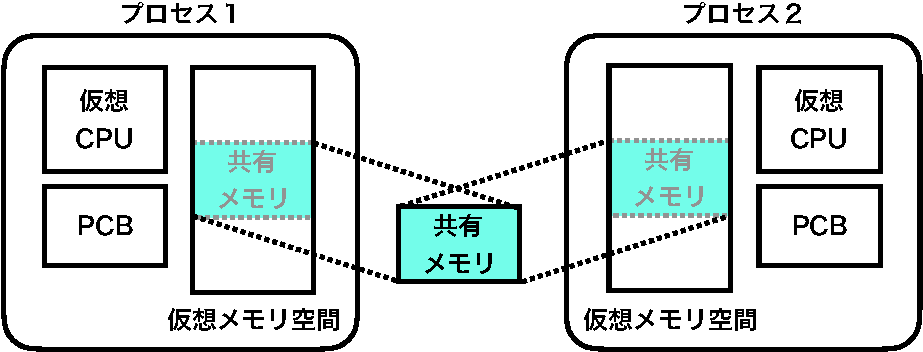
\includegraphics[scale=0.6]{Fig/ipcShearedMemory-crop.pdf}
\end{myfig}

メモリ管理のハードウェア(Memory Management Unit : MMU)\footnote{
  MMUに付いては「第\ref{memoryManagement}部 メモリ管理」で解説する.
}を適切に設定することで,
複数のプロセスの仮想メモリ空間に同じ物理メモリを貼り付ける.
メモリを貼り付ける操作はシステムコールを用いて行う.
貼り付けが完了した後は,
システムコールを用いることなく情報の共有が可能であるが,
プロセス間の同期機構は別に準備する必要がある.

\subsection{UNIXの共有メモリ関連システムコール等}
UNIXの共有メモリ関連のシステムコールとライブラリ関数を
\figref{ipcUnixSharedMemory}に紹介する.

\begin{myfig}{btp}{UNIXの共有メモリ関連システムコールとライブラリ関数}
  {ipcUnixSharedMemory}
  \lstinputlisting[numbers=none]{Lst/ipcUnixSharedMemory.txt}
\end{myfig}

\begin{quote}
  \begin{description}
  \item [\texttt{ftok()}ライブラリ関数]
    \|ftok()|は,\|path|と\|id|の組合せからから,
    システム内で一意な\|key|値を生成する.

  \item [shmgetシステムコール]
    \|key|値で識別される共有メモリセグメントのID返す.
    \|key|値で識別される共有メモリセグメントが存在しない場合は,
    \|size|バイトのものを新しく作ることも可能である.
    \|flag|の値は共有メモリのアクセス許可ビット(\|rwxrwxrwx|)と,
    \|IPC_CREAT|等のフラグである.

  \item [shmatシステムコール]
    共有メモリセグメントをID(\|shmId|)で指定し,
    プロセスの仮想アドレス空間に貼り付ける.

  \item [shmdtシステムコール]
    共有メモリセグメントをアドレス(\|addr|)で指定し,
    プロセスの仮想アドレス空間から取り除く.

  \item [shmctlシステムコール]
    共有メモリセグメントをID(\|shmId|)で指定し操作する.
    共有メモリセグメントの削除等の操作ができる.
  \end{description}
\end{quote}

\subsection{UNIXの共有メモリ使用例}
共有メモリセグメントを作成し,
そこから定期的にデータを読み出し表示するサーバプログラムの例を
リスト\ref{ipcUnixSharedMemoryServer}に示す\footnote{
  ここで示すプログラムは macOS 10.13.2 で動作確認してあるが,
  他のUNIXでも動作するはずである.}.
また,サーバプログラムが作成した共有メモリセグメントにデータを書き込む
クライアントプログラムの例を
リスト\ref{ipcUnixSharedMemoryClient}に示す.

\lstinputlisting[numbers=left,float=btp,label=ipcUnixSharedMemoryServer,
  caption=UNIXの共有メモリサーバ例]
  {SampleCode/UnixSharedMemory/ipcUnixSharedMemoryServer.c}

\lstinputlisting[numbers=left,float=btp,label=ipcUnixSharedMemoryClient,
  caption=UNIXの共有メモリクライアント例]
  {SampleCode/UnixSharedMemory/ipcUnixSharedMemoryClient.c}

サーバプログラムでは,
28行の\|printf()|が共有メモリ(\|data|)から文字列を読み出し表示する.
文字列が\|end|ならプログラムを終了する.
クライアントプログラムでは,
27行の\|fgets()|が共有メモリ(\|data|)に文字列を書き込む.
これらのプログラムでは,
共有メモリが普通の文字配列のように\|printf()|や\|fgets()|に渡されている.
共有メモリなので,
\|fgets()|が書き込んだ内容を\|printf()|が読み出すことになる.

実行例は\figref{ipcUnixSharedMemoryTest}のようになる.
図は二つのターミナルを開いて操作した状態を示している.
左半分が第一のターミナル,
右半分が第二のターミナルである.
まず,左のターミナルで
サーバプログラム(ipcUnixSharedMemoryServer)を起動する.
これで共有メモリセグメントが準備された.
次に,右のターミナルで
クライアントプログラム(ipcUnixSharedMemoryClient)を起動する.
この状態で右のターミナルに入力した文字列が,
クライアントプログラムにより共有メモリに書き込まれる.
左のターミナルで実行中のサーバプログラムは,
共有メモリの内容を定期的に表示する.

\begin{myfig}{btp}{UNIXのメモリ共有プログラム実行例}{ipcUnixSharedMemoryTest}
  \lstinputlisting[numbers=none]{Lst/ipcUnixSharedMemoryTest.txt}
\end{myfig}

ここに紹介した簡単なプログラムでは,
クライアントプロセスがデータを書き換え中に,
サーバプロセスがデータを読み出す可能性がある.
\emph{このようなプログラムを使用してはならない.}
実際に使用する場合は書き換え中のデータを読み出さないように,
セマフォ等\footnote{UNIXではセマフォも使用できる.}を
用いて相互排除を行う必要がある.
原理の確認以外の目的に,\emph{このプログラムを使用してはならない.}

%==============================================================================
\section{メッセージ通信}
メッセージ通信は\figref{ipcMessagePassing}に示すように,
システムコールを用いてプロセス間で情報をコピーする方式である.
プロセス1はsendシステムコールを用いてプロセス2へメッセージを送る.
プロセス2はreceiveシステムコールを用いてプロセス1からメッセージを受取る.
メッセージ通信は,
データを送る度にシステムコールを使用するのでオーバーヘッドが大きいが,
プロセス間の同期機構としても働く.

\begin{myfig}{btp}{メッセージ通信}{ipcMessagePassing}
  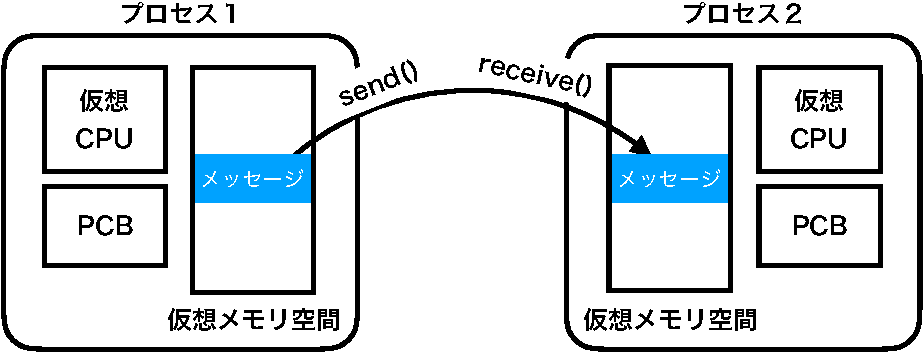
\includegraphics[scale=0.6]{Fig/ipcMessagePassing-crop.pdf}
\end{myfig}

\subsection{通信相手の指定方式(Naming)}
メッセージの通信相手を指定する方式が二つある.

\begin{quote}
  \begin{description}
  \item[直接指定方式]
    相手プロセスを直接指定する方式である.
    \figref{ipcDirect}は直接指定方式を表している.
    send,receiveシステムコールの引数は,
    \emph{相手プロセス}と\emph{メッセージ}になる.
    \emph{相手プロセス}として\|ANY|のような記述を許すことで,
    多対多の通信も可能である.
    また,受信したメッセージをいくつか貯めることが可能な,
    バッファ付きの通信方式もあり得る.
    \begin{myfig}{btp}{直接指定方式}{ipcDirect}
      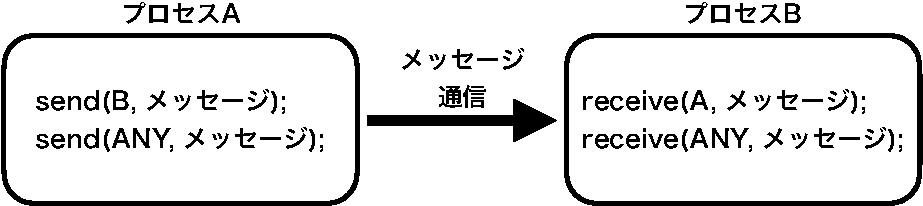
\includegraphics[scale=0.6]{Fig/ipcDirect-crop.pdf}
    \end{myfig}
  \item[間接指定方式]
    \emph{リンク(ポート,ソケット,チャネルとも呼ばれる)}を作成し,
    通信先としてリンクの名前を用いる方式である.
    \figref{ipcIndirect}は間接指定方式を表している.
    send,receiveシステムコールの引数は,
    \emph{リンク}と\emph{メッセージ}になる.
    同じリンクを共有する複数のプロセスが存在すると,
    自然に多対多の通信方式が実現できる.
    リンクにメッセージをいくつか貯めるバッファ機能を持たせる.
    %UNIXのソケットやパイプはこの方式によく似ている.
    \begin{myfig}{btp}{間接指定方式}{ipcIndirect}
      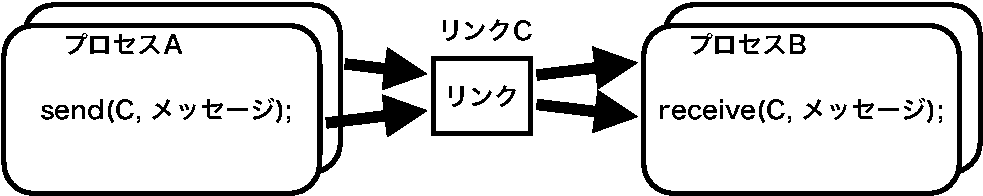
\includegraphics[scale=0.6]{Fig/ipcIndirect-crop.pdf}
    \end{myfig}
  \end{description}
\end{quote}

\subsection{バッファリング(Buffering)}
直接指定方式か間接指定方式かに関わりなく,
メッセージを格納するバッファを用意することができる.
送信プロセスはバッファに空きがあれば待ち時間なしに
sendシステムコールを完了できる.
受信プロセスはバッファにメッセージがあれば待ち時間なしに
receiveシステムコールを完了できる.

間接指定方式ではリンクがバッファを持つと考え,
リンクを作成する時点でバッファの大きさを指定する場合が多い.
\figref{ipcIndirect}で「リンク」の位置にバッファがあると考えると分かりやすい.

\subsection{メッセージの形式}
通信に用いられるメッセージの形式には次の選択肢がある.

\begin{quote}
  \begin{description}
  \item [メッセージ長] \emph{固定長方式}または\emph{可変長方式}
  \item [メッセージ形式] \emph{タグ付き}または\emph{タグなし}
  \end{description}
\end{quote}

\emph{タグ}は種類を表すためにメッセージに付加されるデータのことである.
タグ付きのメッセージ通信機構では,
送信側はメッセージにタグを付加する.
受信側はタグを指定してメッセージを選択的に受信することができる.

\subsection{同期方式(Synchronization)}
\emph{非同期方式(ノンブロッキング:Nonblocking)}と
\emph{同期方式(ブロッキング:Blocking)}の二つがある.
同期式の特別な場合としてバッファを用いない\emph{ランデブー方式}も考えられる.

\begin{quote}
  \begin{description}
  \item [非同期方式]
    \|send()|はバッファに空きがない場合エラーで終了する.
    \|receive()|はバッファにメッセージがない場合エラーで終了する.
  \item [同期方式]
    \|send()|はバッファに空きがない場合はブロックし,空きができるのを待つ.
    \|receive()|はバッファにメッセージがない場合はブロックし,
    メッセージが届くのを待つ.
  \item [ランデブー方式]
    \|send()|は受信プロセスが\|receive()|を実行するまでブロックする.
    \|receive()|は送信プロセスが\|send()|を実行するまでブロックする.
    両方のプロセスが\|send()|と\|receive()|を
    実行したらプロセス間でメッセージをコピーする.
    プロセス間で直にメッセージをコピーするので,
    バッファは不要である.
  \end{description}
\end{quote}

\subsection{UNIXのメッセージ通信システムコール}
UNIXでは複数種類のメッセージ通信機構が利用可能である.
ここでは,System V 系のUNIXを起原とする方式を紹介する.
この方式は,\emph{間接指定方式},\emph{バッファリングあり},
\emph{可変長},\emph{タグ付き}の方式である.
システムコールの引数によって,
\emph{同期方式}と\emph{非同期方式}のどちらにも対応することができる.
UNIXのメッセージ通信関連のシステムコール等を\figref{ipcUnixMessage}に示す.

\begin{myfig}{btp}{UNIXのメッセージ通信関連システムコールとデータ構造}
  {ipcUnixMessage}
  \lstinputlisting[numbers=none]{Lst/ipcUnixMessage.txt}
\end{myfig}

\begin{quote}
  \begin{description}
  \item [msgBuf構造体]
    ユーザが宣言する構造体である.
    必ず,long型の\|mtype|フィールドから始める必要がある.
    このフィールドが\emph{タグ}の役割を持つ.
    \|mtext|はメッセージの本体を格納する領域であり,
    ユーザが自由に大きさや用途を決めることができる.
  \item [msggetシステムコール]
    リンク(メッセージキューと呼ぶ)のIDを返す.
    \|key|は,共有メモリの場合と同様に\|ftok()|関数を用いて生成した値である.
    メッセージキューを識別するために用いる.
    \|msgflg|に\|IPC_CREAT|を指定すると,メッセージキューを新規に作成する.
  \item [msgsndシステムコール]
    \|msqid|で指定したメッセージキューにメッセージを送信する.
    \|msgp|に送信するメッセージを格納した\|msgBuf|構造体のポインタを渡す.
    メッセージは\emph{可変長方式}なので\|msgsz|で長さを指定する.
    \|msgsz|は構造体全体ではなく,構造体の\|mtext|部分のバイト数である.
    \|msgflg|に\|IPC_NOWAIT|フラグを指定すると\emph{非同期方式}になり,
    指定しないと\emph{同期方式}になる.
  \item [msgrcvシステムコール]
    \|msqid|で指定したメッセージキューからメッセージを受信する.
    \|msgp|に受信したメッセージを格納する\|msgBuf|構造体のポインタを渡す.
    \|msgsz|は受信可能な\|mtext|の最大バイト数である.
    \|msgtyp|に受信したいメッセージの\|mtype|を指定し,
    \emph{タグ}が合致するメッセージを選択的に受信できる.
    \|msgflg|に\|IPC_NOWAIT|フラグを指定すると\emph{非同期方式}になる.
  \item [msgctlシステムコール]
    \|msqid|で指定したメッセージキューに対して操作を行う.
    \|cmd|に操作の種類(コマンド),
    \|buf|にコマンドのパラメータを渡す.
    \|IPC_RMID|コマンドを指定するとメッセージキューの削除ができる.
  \end{description}
\end{quote}

\subsection{UNIXのメッセージ通信プログラム例}
メッセージを表現する構造体の例をリスト\ref{ipcUnixMessageH}に示す\footnote{
  ここで紹介するプログラムはmacOS 10.13.2 で動作確認した.
  macOSのオンラインマニュアルには,
  ここで紹介するメッセージ通信方式について記載がないが,
  試してみると使用できた.}.
メッセージ本体の長さは\|MAXMSG|に定義している.
以下のプログラムは,メッセージ長をこの値に固定した例になっている.

\lstinputlisting[caption=UNIXのメッセージ通信プログラム例(メッセージ構造体),
  numbers=left,float=btp,label=ipcUnixMessageH]
  {SampleCode/UnixMessage/ipcUnixMessage.h}

リスト\ref{ipcUnixMessageWriter}に
メッセージキューを作成しメッセージを書き込むプログラムの例を示す.
このプログラムは入力した文字列をメッセージ本体に格納して
メッセージキューに送信する.
タグの役割を持つ\|mtype|は常に1にしている.

\lstinputlisting[numbers=left,float=btp,label=ipcUnixMessageWriter,
  caption=UNIXのメッセージ通信プログラム例(メッセージ送信側)]
  {SampleCode/UnixMessage/ipcUnixMessageWriter.c}

リスト\ref{ipcUnixMessageReader}に,
メッセージキューからメッセージを読み込み内容を表示するプログラムの例を示す.
22行で\|msgtyp|を0にして\|msgrcv()|を実行している.
\|msgtyp|が0の場合は,
メッセージの\|mtype|(タグ)を無視して
メッセージキューの先頭から順にメッセージを受信する.
26行で\|mtype|と\|mtext|の内容を表示している.
送信側のプログラムがメッセージキューを削除すると
22行でエラーが発生し24行で終了する.

\lstinputlisting[numbers=left,float=btp,label=ipcUnixMessageReader,
  caption=UNIXのメッセージ通信プログラム例(メッセージ受信側)]
  {SampleCode/UnixMessage/ipcUnixMessageReader.c}

\subsection{UNIXのメッセージ通信プログラムの実行例}
メッセージ通信プログラムの実行例を
\figref{ipcUnixMessageTest}に示す.
図は二つのターミナルを開いて操作した状態を示している.
左半分が第一のターミナル,
右半分が第二のターミナルである.
まず,左のターミナルで送信プログラム(ipcUnixMessageWriter)を起動する.
これでメッセージキューが準備された.
次に,右のターミナルで受信プログラム(ipcUnixMessageReader)を起動する.
この状態で左のターミナルに入力した文字列が,
メッセージ通信を用いて右のターミナルで実行中のプログラムに送信される.
右のターミナルには
受信したメッセージの\|mtype|と\|mtext|の内容が表示される.

\begin{myfig}{btp}{UNIXのメッセージ通信プログラム実行例}{ipcUnixMessageTest}
  \lstinputlisting[numbers=none]{Lst/ipcUnixMessageTest.txt}
\end{myfig}

%==============================================================================
\section{メッセージ通信機構の実装例}
第\ref{tacosIPC}章に
TacOSにおけるメッセージ通信機構の実装例を紹介する.
TacOSのメッセージ通信機構はセマフォを利用して実装されている.

%==============================================================================
\section{まとめ}
この章ではプロセス間通信(IPC)について学んだ.
IPCには共有メモリとメッセージ通信の二種類があった.
UNIXの共有メモリとメッセージ通信についてプログラム例を示した.

%==============================================================================
\section*{練習問題}
\begin{enumerate}
  \renewcommand{\labelenumi}{\ttfamily\arabic{chapter}.\arabic{enumi}}
  \setlength{\leftskip}{1em}
\item 次の言葉の意味を説明しなさい.
  \begin{enumerate}
  \item 共有メモリ
  \item メッセージ通信
  \item 直接指定方式
  \item 間接指定方式
  \item バッファリング
  \item 同期方式
  \item 非同期方式
  \item ランデブー方式
  \item メッセージのタグ
  \end{enumerate}
\item プロセス間の共有メモリとスレッド間の共有変数の違いは何か?
\item UNIXの共有メモリ使用例
  (リスト\ref{ipcUnixSharedMemoryServer},
    リスト\ref{ipcUnixSharedMemoryClient})
  を実際に実行し動作確認しなさい.
  なお,ソースプログラムは以下から入手可能である. \\
  \url{\git/SampleCode/UnixSharedMemory}
\item 動作確認したプログラムでは,
  サーバプログラムは共有メモリが変更されたことを確認しないで,
  一定の時間間隔で共有メモリの内容を表示している.
  \begin{enumerate}
  \item どのような不都合が予想されるか?
  \item クライアントとサーバで同期をする方法はあるか?
  \end{enumerate}
\item メッセージ通信でバッファを大きくすることのメリットは何か?
\item UNIXのメッセージ通信プログラム例(リスト\ref{ipcUnixMessageH},
  リスト\ref{ipcUnixMessageWriter},リスト\ref{ipcUnixMessageReader})
  を実際に実行し動作確認しなさい.
  なお,ソースプログラムは以下から入手可能である. \\
  \url{\git/SampleCode/UnixMessage}
\item UNIXのメッセージ通信プログラム例は生産者と消費者の問題の解になっている.
  複数生産者と複数消費者の問題の解にもなっているか?
\item UNIXのメッセージ通信プログラム例が
  複数生産者と複数消費者の問題の解にもなっているか,
  動作確認する手順を説明しなさい.
\end{enumerate}
 % プロセス間通信
\chapter{モニタ}
\label{monitor}
複数のプロセス(スレッド)で資源を共有する際に,
プロセスの同期や相互排除にセマフォを用いることを既に学んだ.
しかし,
セマフォは基本的な機能を提供するだけで使い方はプログラマ任せなので,
間違った使用がされる可能性が高い.
その結果,
タイミングに依存した発見の難しいバグを持ったプログラムが作成される.
そこで,プログラミング言語と一体になり\footnote{
本章の話題はオペレーティングシステムではなくプログラミング言語である.},
プログラマに同期機構を強制的に利用させる仕組みが考案された.
そのような仕組みの一つとして{\bf モニタ(Monitor)}を紹介する.

\section{概要}
モニタはリソース管理用の機能と制約を持った
{\bf 抽象データ型}\cite{AbstractDataType}である.
C++やJavaなどを学んだことのある人なら,
「抽象データ型はクラスのこと」と言えば分かりやすいと思われる.

モニタは抽象データ型の一種であるが,
プロセス(スレッド)間の同期を行う機構が予め組込まれ,
その制約の下で使用するものである.
モニタの特長を以下に箇条書きにする.
% その中で,最初の二つは抽象データ型に一般的な特長である.
% 最後の一つはモニタ独特の特長である.

\begin{itemize}
\item プログラマが定義できる型である.(抽象データ型で一般的)
\item データと操作をまとめて定義する.(抽象データ型で一般的)
\item 同期のための機能が組込まれている.(モニタ独特)
\end{itemize}

なお,
Javaのクラスは同期のための機構も持っており,
一定のルールに従って使用すればモニタに近い使用もできる.
%(ただし,完全ではモニタない.)
モニタをサポートするプログラミング言語は Concurrent Pascal が有名である.

\section{構成要素}
モニタは次の要素を持つ抽象データ型である.
\figref{monitor}にモニタの模式図\footnote{
\figref{monitor}では,初期化プログラムが省略してある.}を示す.

\begin{itemize}
\item 資源(データ,変数)
\item 手続き(操作,メソッド)
\item ガード
\item 条件変数
\end{itemize}

\myfigure{btp}{scale=0.6}{Fig/monitor-crop.pdf}{モニタの模式図}{monitor}

\subsection{資源(データ,変数)}
複数のスレッドによって共有される変数のことである.
モニタの内部に必要に応じて名前付きで宣言する.
モニタの外から直接アクセスすることはできない.

\subsection{手続き(操作,メソッド)}
外部から呼び出されるプログラムである.
モニタの内部に必要に応じて名前付きで定義する.
モニタの外部から資源にアクセスできるインタフェースは手続きだけである.
手続きの実行は{\bf ガード}の働きにより排他的に行われ,
同時に実行される手続きは必ず一つ以内である.

\subsection{ガード}
モニタに一つのガードが存在し,
手続きを排他的に実行するために用いられる.
手続きを実行するときは自動的にガードにロックがかけられる.
複数のスレッドが同時にモニタに入ることはできない.
%これにより複数のスレッドが同時にモニタの手続きを実行しないようにする.

\subsection{条件変数}
モニタの内部に必要に応じて名前付きで宣言する.
条件変数にはwaitとsignalの二つの操作ができる.
wait操作を行ったスレッドは{\bf ガードを外して}条件変数の待ち行列に入る.
signal操作は条件変数の待ち行列から一つのスレッドを選んで実行可能にする.
実行可能になったスレッドは{\bf ただちに}実行を再開する.
待ち行列にスレッドが複数ある時,
どのスレッドが実行可能になるか明確な決まりはない.

\subsection{初期化プログラム}
モニタのインスタンスを作成する時に,
初期化のために実行されるプログラムである.

\section{相互排除問題の解}
前出の架空の銀行口座管理プログラムの例をモニタに置換える.
残高がスレッド間で共有される変数である.
共有変数をスレッド間で安全に共有させるためにモニタを用いる.

\subsection{共有変数の記述}
\figref{monAccount}にJava風の仮想言語による銀行口座の記述を示す.
本物の口座は他にも情報を持っているだろうが,
ここでは口座は残高だけ持っていることにする.

\begin{myfig}{btp}{モニタによる相互排除の実現(仮想言語版)}{monAccount}
\lstinputlisting[numbers=left]{Lst/MonAccount.jama}
\end{myfig}

\begin{description}
\item [2行]
この仮想言語では,Java の class 定義に似た monitor 定義ができるものとす

\item [3〜4行]
{\bf 資源}の例である.
この例では残高を表すスレッド間の共有変数({\tt money})が資源である.

\item [5〜8行]
{\bf 初期化プログラム}の例である.
モニタのインスタンス生成時に残高を引数で初期化する.

\item [9〜15行]
{\bf 手続き}の例である.
手続きは共有資源を書換えるので{\bf クリティカルセクション}であるが,
自動的に{\bf ガード}をロックし排他的に実行されるので
{\bf 明示的な相互排除を行う必要はない}.
\end{description}

\subsection{共有変数の利用}
\figref{monAccountMain}に,
\figref{monAccount}で定義した\|MonAccount|モニタを
利用した相互排除問題の解を示す.

\begin{myfig}{btp}{モニタによる相互排除の利用(仮想言語版)}{monAccountMain}
\lstinputlisting[numbers=left]{Lst/MonAccountMain.jama}
\end{myfig}

\begin{description}
\item [2行]
\figref{monAccount}に示した\|MonAccount|モニタ型のインスタンスを生成する.

\item [3〜8行]
入金管理スレッドが実行するメソッドである.
入金額を受信し口座に入金する.

\item [9〜13行]
引落し管理スレッドが実行するメソッドである.
支払い金額を受信し口座から引落す.

\item [14〜17行]
プログラムは\|main()|から実行を開始する.
\|main()|では「入金管理スレッド」と「引落し管理スレッド」を起動する.
これらのスレッドがそれぞれ,
\|receiveThread()|メソッドと\|payThread()|メソッドを実行するものとする.
\end{description}

\section{生産者と消費者問題の解}
この問題で{\bf 資源}はデータを保管するFIFO構造のバッファである.
このバッファを以下では{\bf キュー}と呼ぶことにする.
キューとキューを操作する手続きは,
全てモニタの中にまとめられる.
キューを使用するユーザプログラムには,
排他や同期に関わる難しいプログラムが含まれない.
資源の操作に関する難しいプログラムが一箇所にまとめられることも,
モニタを使用するメリットである.

以下では生産者と消費者問題の解を示すために,
まず,データのバッファになるキューをモニタを用いて記述する.
次に,キューを使用する生産者スレッドと消費者スレッド作る.

\subsection{キューの記述}
\figref{monProducerConsumer}にJava風の仮想言語によるキューの記述例を示す.
このプログラムは次のようになっている.

\begin{myfig}{btp}{モニタによるキューの実現(仮想言語版)}{monProducerConsumer}
\lstinputlisting[numbers=left]{Lst/BoundedBuffer.jama}
\end{myfig}

\begin{description}
\item [1行] この仮想言語では,
Javaの\|class|定義に似た\|monitor|定義ができるものとする.

\item [2〜5行] {\bf 資源}の例である.
キューとして使用するリングバッファのデータ構造を宣言している.
このモニタの目的は,資源であるキューを管理することである.
手続きを介すること無しに資源にアクセスすることは禁止なので,
モニタの外部からこれらのデータにアクセスできない.
\|N|がバッファの大きさ,
\|buf|がバッファ本体,
\|first|がバッファ中の次のデータ読みだし位置,
\|last|がバッファ中の次のデータ書込み位置,
\|cnt|がバッファ中のデータ件数を表す.

\item [6〜8行] {\bf 条件変数}の例である.
この仮想言語では,\|Condition|型の変数として条件変数を宣言する.
\|empty|は,
キューが空の時にデータを取り出そうとしたスレッドが,
キューにデータが書き込まれるまで待つために使用する条件変数である.
\|full|は,
キューが満杯の時にデータを書き込もうとしたスレッドが,
キューに空きができるまで待つために使用する条件変数である.

\item [9〜14行] {\bf 初期化プログラム}の例である.
モニタのインスタンスを作る際に実行されるものとする.
引数はバッファの大きさである.

\item [15〜30行] {\bf 手続き}の例である.
手続きはモニタの外部から呼び出し可能なプログラムである.
\|append()|はキューにデータを追加する.
\|remove()|はキューからデータを取り出す.
これらのプログラムが実行される時は{\bf ガード}による排他制御がされる.
次にバッファが満杯で待ちが発生する例を考えてみる.

データをキューに追加するために\|append()|を呼出したスレッドは,
コメントに\|(1)|と記された行を実行し,
キューが満杯の時17行の\|full.wait()|で待ち状態になる.
待ち状態になる時はガードを外すので,
他のスレッドがモニタに入ることができる.

他のスレッドがデータをキューから取り出すために\|remove()|を呼び出すと,
\|(2)|の行が実行され28行の\|full.signal()|まで進む.
\|full.signal()|が実行されると待ち状態のスレッドが一つ起床し,
\|(3)|の行が{\bf ただちに}実行される.
\|(3)|の実行が終了した後に(4)の行が実行される.
{\bf \|(2)|から\|(4)|の実行の間,
ガードは外さないので他のスレッドがモニタに入ることはない.}

\end{description}

\subsection{生産者と消費者スレッドの記述}
\figref{monProducerConsumerMain}に
Java風の仮想言語による生産者と消費者問題の解を示す.
このプログラムは\figref{monProducerConsumer}で定義したキューを使用する.

\begin{myfig}{btp}{モニタによる生産者と消費者問題の解(仮想言語版)}
{monProducerConsumerMain}
\lstinputlisting[numbers=left]{Lst/BoundedBufferMain.jama}
\end{myfig}

\begin{description}
\item [2行] 
\figref{monProducerConsumer}に示した
\|BoundedBuffer|モニタ型のインスタンスである.

\item [3〜8行]
生産者スレッドが実行するメソッドである.
無限にデータを生産し\|queue|に追加し続ける.

\item [9〜14行]
消費者スレッドが実行するメソッドである.
\|queue|からデータを取出し処理することを無限に繰り返す.

\item [15〜18行]
プログラムは\|main()|から実行を開始する.
\|main()|では「生産者スレッド」と「消費者スレッド」を起動する.
これらのスレッドがそれぞれ,
\|producer()|メソッドと\|consumer()|メソッドを実行する.

\end{description}

\section{セマフォによるモニタの実装}
モニタの仕組みをより正確に理解するために,
セマフォによるモニタの実装方法を考えてみる.
\figref{monProducerConsumer}の仮想言語で記述されたモニタを
Javaクラスに書換えたものを
\figref{semProducerBuffer1}と\figref{semProducerBuffer2}に示す.
モニタをサポートする言語のコンパイラは,
自動的にこのような変換を行っている.

\begin{myfig}{btp}{モニタと同等なキューをセマフォで実現(Java版,前半)}
{semProducerBuffer1}
\lstinputlisting{Lst/SemBoundedBuffer.java1}
\end{myfig}

\begin{myfig}{btp}{モニタと同等なキューをセマフォで実現(Java版,後半)}
{semProducerBuffer2}
\lstinputlisting[firstnumber=last]{Lst/SemBoundedBuffer.java2}
\end{myfig}

\subsection{モニタ機能のJavaによる実装}
\figref{semProducerBuffer1}に\|SemBoundedBuffer|クラスが
モニタと同等な動作をするために必要な機能の実装を示す.

\begin{description}
\item [1行]
\|java.util.concurrent|パッケージの\|Semaphore|クラスを使用する.
\|Semaphore|クラスはカウンティングセマフォ型である.

\item [2行]
セマフォを使用したキュークラスを\|SemBoundedBuffer|と名付ける.

\item [3行]
セマフォ(\|guard|)はモニタのガードの役割りを持っている.
スレッドは,モニタ(\|SemBoundedBuffer|クラス)内の手続き(メソッド)を実行する前に,
\|guard|をロックする.

\item [4〜5行]
モニタの条件変数に\|signal()|操作を行った時,
条件変数で待っていたスレッドがあれば{\bf ただちに}実行しなければならない.
待っていたスレッドを先に実行させるために,
\|signal()|操作を行ったスレッドを待ちにするセマフォ(\|next|)と
\|next|を待っているスレッドの数を記憶する変数(\|nextCont|)を準備する.

\item [6行]
{\bf 条件変数型}(\|Condition|)を内部クラスとして定義する.

\item [7〜8行]
条件変数にwait操作を行った時に
スレッドを待ち状態にするためのセマフォ(\|sem|)と
待っているスレッドの数をカウントする変数(\|count|)である.

\item [9行]
\|await()|は条件変数のwait操作を行うメソッドである.
Javaの\|Object|クラスに別の\|wait()|メソッドが定義さているので,
名前を\|await|にした.

\item [11〜15行]
\|release()|はセマフォにV操作を行う.
%\|Semaphore|クラスのインスタンスメソッドである.
\|nextCont|は\|signal()|中で待っているスレッドの数である.
待っているスレッドがある場合は起こす.
そうでなければモニタのガードを外す.

\item [16行]
\|acquireUninterruptibly()|はセマフォにP操作を行う.
%\|Semaphore|クラスのインスタンスメソッドである.
\|sem|は初期値0のセマフォなので,
\|await()|を呼出したスレッドがここでブロックする.

\item [19行]
条件変数にsignal操作を行うメソッドである.

\item [20〜25行]
条件変数を待っているスレッドの数(\|count|)を調べ,
1以上なら22行で起床させる.
自身は23行でブロックし,
起床したスレッドが\|exitProc()|を実行しモニタを出るのを待つ.

\item [28行]
モニタ手続きの最後の行で呼び出すメソッドである.
\|signal()|中の23行でブロックしているスレッドがあれば起床させる.
なければモニタのガードを外す.

\end{description}

\subsection{モニタ機能の使用}
\figref{semProducerBuffer2}に\|SemBoundedBuffer|クラスの後半を示す.
ここでは,\|SemBoundedBuffer|クラスの前半で定義したモニタ機能を使用している.

\begin{description}
\item [35〜38行]
{\bf 資源}(リングバッファ)を表現するための変数を宣言する.
モニタ(クラス)の外部から資源を隠蔽するために
\|private|修飾子を付けて宣言する.

\item [39〜41行]
{\bf 条件変数}は
前半で定義した\|Condition|クラスのインスタンス変数である.

\item [42〜47行]
{\bf 初期化}はクラスのコンストラクタとして実装する.

\item [48〜67行]
{\bf 手続き}は仮想言語で定義したものに,
50行と59行の「ガード取得」,
56行と65行の「手続きの出口処理」が追加されている.

\end{description}

% \section{Javaのモニタ風機構によるリーダ・ライタ問題の解}
% モニタについて理解を深めるために,
% 仮想言語によるリーダ・ライタ問題の解を示す.
% 
% \begin{myfig}{btp}{モニタによるリータ・ライタの問題(仮想言語版)}
% {monProducerConsumerMain}
% \lstinputlisting[numbers=left]{Lst/BoundedBufferMain.jama}
% \end{myfig}

\section{Javaのモニタ風機構による生産者と消費者問題の解}
Java言語はモニタに似た同期機構をサポートしている.
\figref{javaMonProducerConsumer}にJavaによる生産者と消費者問題の解を示す.
Javaには{\bf 条件変数}に相当するものが無い.

\begin{myfig}{btp}{Javaのモニタ風機構による生産者と消費者問題の解}
{javaMonProducerConsumer}
\lstinputlisting[numbers=left]{Lst/MonBoundedBuffer.java}
\end{myfig}

\begin{description}
\item [1行]
Javaのモニタ風機構を利用したキュークラスを\|MonBoundedBuffer|と名付ける.

\item [2〜5行]
{\bf 資源}(リングバッファ)を表現するための変数を宣言する.
クラスの外部から資源を隠蔽するために\|private|修飾子を付けて宣言する.

\item [6〜11行]
{\bf 初期化}をコンストラクタとして実装する.

\item [13行]
クラスの内部だけで呼び出す\|private|なメソッドである.
\|await()|メソッドは条件変数の\|wait()|に似た働きをする.

\item [14行]
\|await()|メソッドは\|Object|クラスの\|wait()|メソッドを呼び出す.
Javaオブジェクトは暗黙の条件変数が一つあるような構造になっている.
\|wait()|メソッドは暗黙の条件変数の待ち行列\footnote{
Javaでは待機セットと呼ぶ.}にスレッドを入れる.
\|wait()|メソッドは割込みなどでも終了するのでtry-catch構文で使用する.

\item [16,23行]
外部から呼び出すことができるメソッドは\|synchronized|修飾子を付けて定義する.
\|synchronized|メソッドは{\bf モニタの手続き}と同様に,
オブジェクトの{\bf ガード}をロックした\footnote{
Javaではモニタを所有すると言う.}スレッドだけが実行できる.
オブジェクトのガードをロックできない場合はガードの待ち行列に入る.

\item [17行]
バッファが満杯の場合に\|await()|を用いて暗黙の条件変数で待ち状態になる.
\|await()|は割込みなど別の理由でも終了するので,
バッファに空きができるまで繰り返し\|await()|を呼び出す.

\item [21行]
\|notify()|は暗黙の条件変数の\|signal()|に相当する.
暗黙の条件変数は一つしかないので,
スレッドが\|remove()|で待ちになっている可能性ある
(直前までバッファが空だった)場合だけ\|notify()|するようにしている.
無条件に\|notify()|を実行するようにすると,
\|append()|で複数のスレッドが待ちになっている場合に,
それらを起床させてしまう.

\item [24行]
バッファが空の場合に\|await()|を用いて暗黙の条件変数で待ち状態になる.

\item [28行]
暗黙の条件変数は一つしかないので,
スレッドが\|append()|で待ちになっている可能性ある
(直前までバッファが満杯だった)場合だけ\|notify()|するようにしている.

\item [29行]
取り出したデータを呼出し側に返す.
16行から28行の右端に書いてあるコメントは\figref{monProducerConsumer}と同様に,
生産者スレッドが17行でブロックした後,
消費者スレッドが28行で生産者スレッドを起床させるときの実行順である.
これまでの例と比較して29行が異なっている.
Javaの\|notify()|はモニタの\|signal()|と異なり,
\|synchronized|メソッドの最後まで実行した後,
スレッドの切換えが起こるからである.
\end{description}

\section{まとめ}
モニタについて学んだ.
モニタはスレッド間の同期と相互排除に使用できる
「高級言語に組込まれた仕組み」である.
モニタ内に資源と,資源を操作する手続きを記述する.
資源の相互排除と同期に関わる難しい処理が
プログラムのあちこちに分散しない.
また,モニタ内の手続き(プログラム)の実行は自動的に相互排除されるので,
クリティカルセクションを明示する必要もない.

モニタで記述した「生産者と消費者問題」の解を,
セマフォを用いて実装し直す例を示した。
この例をよく観察するとモニタの動作が細部まで理解できる.

Java言語はモニタに似た機能をサポートする言語であるが,
資源が外部からアクセスできないように\|private|修飾が必要なこと,
条件変数がないこと,
\|wait()|が\|signal()|以外でも終了すること,
\|signal()|を実行した後手続きの最後まで実行されること
等が異なる.

\section*{練習問題}
\begin{enumerate}
\renewcommand{\labelenumi}{\tt \arabic{chapter}.\arabic{enumi}}
 \setlength{\leftskip}{1em}

\item {\bf 抽象データ型}の定義を調べなさい.

\item \figref{monProducerConsumer}のプログラムにおいて,
{\tt cnt}なしにキュー(リングバッファ)を記述できるか?

\item \figref{monProducerConsumer}のプログラムにおいて,
キューが空のとき一つのスレッドが{\tt remove()}を実行した.
その後,別のスレッドが{\tt append()}を実行した.
この時の{\tt append()},{\tt remove()}内が実行される順を答えなさい.

\item \figref{monProducerConsumer}のプログラムは,
複数生産者と複数消費者問題の解に使用できるか?

\item Java風仮想言語のモニタを用いてリーダ・ライタ問題の解を示しなさい.

\item Java風仮想言語のモニタを用いてセマフォを記述しなさい.

\item {\tt semBoundedBuffer}
(\figref{semProducerBuffer1},\figref{semProducerBuffer2})に
メインルーチンを補って実際に実行しなさい.
ソースプログラムは以下から入手できる. \\
\url{https://github.com/tctsigemura/OSTextBook/blob/master/Lst/SemBoundedBuffer.java}

\item {\bf \|signal()|は手続きの最後でしか使用できないことにすると},
{\tt semBoundedBuffer}
(\figref{semProducerBuffer1},\figref{semProducerBuffer2})は
どのように簡略化できるか.

\item {\tt MonBoundedBuffer}(\figref{javaMonProducerConsumer})に
メインルーチンを補って実際に実行しなさい.
ソースプログラムは以下から入手できる.\\
\url{https://github.com/tctsigemura/OSTextBook/blob/master/Lst/MonBoundedBuffer.java}

\item \figref{monProducerConsumer}のプログラムと,
\figref{javaMonProducerConsumer}でコメントに示すように実行順序が異なる.
Javaのモニタ風機構と従来のモニタのどのような違いによるものか?

\item その他に従来のモニタとJavaのモニタ風機構の違いは何があるか?

\item モニタの signal と、セマフォのV操作の違いは何があるか?
\end{enumerate}
 % モニタ
\part{主記憶管理}
\chapter{主記憶(メモリ)}
コンピュータシステムにおいて,
主記憶(メモリ)\footnote{
  本章で「主記憶」と「メモリ」は同じ意味で用いられる.
}はCPUと同様に重要な装置である.
CPUを仮想化し複数のプロセスを同時に実行可能にするには,
主記憶も管理し複数のプロセスに適切に主記憶が割り振られ,
かつ,プロセス同士が干渉しないように分離する必要がある.
この章では主記憶と主記憶管理の基本的なアイデアについて学ぶ.

%==============================================================================
\section{ハードウェア構成}
主記憶はCPUがプログラムを実行する際に,
プログラムの機械語やデータ,スタック領域等を置くメモリのことである.
TeCの主記憶は256バイトのRAM領域であったし,
4年生の実験で使用したH8/3664では32KiBのROMと2KiBのRAMであった.
現代のPCなら4GiBから16GiB程度の大きさを持つ「メモリ」のことである.

本書で前提とする
コンピュタのハードウェア構成は\figref{hardBlock}に示した.
この章ではCPUとメモリに着目するので,
図を単純化し\figref{cpuMemory}のようなモデルを用いる.
この図はCPUがアドレスを指定してメモリのデータを読み書きすることを表している.

\begin{myfig}{btp}{CPUとメモリの関係を表す単純なモデル}{cpuAndMemory}
  \begin{minipage}{0.49\columnwidth}
    \begin{center}
      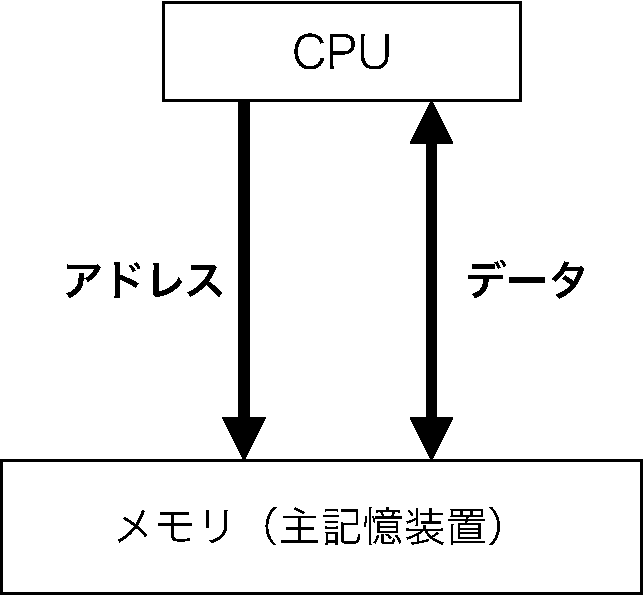
\includegraphics[scale=0.4]{Fig/cpuMemory-crop.pdf}
      \subcaption{単純なモデル}
      \label{fig:cpuMemory}
    \end{center}
  \end{minipage}
  \begin{minipage}{0.49\columnwidth}
    \begin{center}
      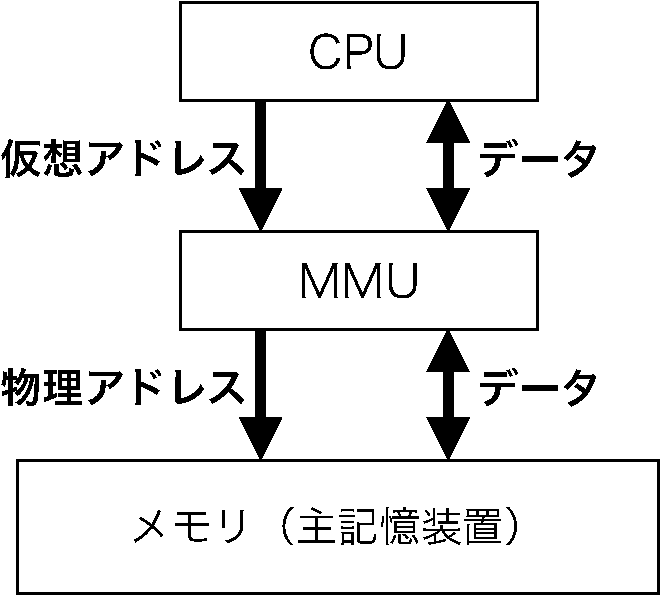
\includegraphics[scale=0.4]{Fig/cpuMmuMemory-crop.pdf}
      \subcaption{仮想化が可能なモデル}
      \label{fig:cpuMmuMemory}
    \end{center}
  \end{minipage}
\end{myfig}

プログラム実行時にCPUは以下のようにメモリをアクセスする.
\begin{enumerate}
\item 命令フェッチ(fetch)\\
  PCの値をアドレスとして出力し主記憶からデータ(命令コード)を\emph{読む}.
\item 命令デコード(decode) \\
  フェッチした命令の種類を調べる.
\item 命令実行(execution)\\
  命令を実行する際に必要に応じてデータのアドレス
  (実効アドレス:Effective Address(EA))を出力し
  主記憶のデータを\emph{読み書きする}.
\end{enumerate}

\figref{cpuMemory}のモデルは,
TeCやH8/3664のようなマイクロコンピュータの様子を表すためには十分である.
しかし,この単純なモデルでは現代の本格的なオペレーティングシステムを
作動させるには次の点で不十分である.
\begin{enumerate}
\item メモリ保護機構がない.\\
  ユーザプロセスがOSのカーネルや,
  他のプロセスを破壊することを防ぐことができない.
\item メモリの再配置機構がない.\\
  同時に複数のプロセスが主記憶にロードされる環境では,
  プロセスの起動と終了が繰り返されるうちに使用できない
  小さなメモリの断片(フラグメント)ができる.
  フラグメントを解消するために,
  実行中プロセスをメモリ内で移動する機能が必要である.
\item 仮想記憶機構が実現できない.\\
  メモリより大きなプログラムを実行するために,
  仮想記憶機構を導入したいができない.
\end{enumerate}

そこで,\figref{cpuMmuMemory}のモデルを用いる.
CPUとメモリの間に
\emph{MMU(Memory Management Unit:メモリ管理装置)}を追加する.
MMUはCPUが出力した\emph{仮想アドレス}をOSが指示したルールに則り
\emph{物理アドレス}に変換してメモリに送るハードウェアである.
\emph{OSの主記憶管理プログラムがMMUを制御することによって,
  使いやすく安全な仮想の主記憶をプロセスに提供する.}

%==============================================================================
\section{メモリ保護機構}
CPUを仮想化したことによって,
複数のユーザプロセスをメモリに同時にロードし並列実行することが可能になった.
これにより,CPUの使用効率が良くなるだけでなく,
コンピュータの使い勝手が非常に良くなった.
しかし,ユーザプログラムのバグや悪意によって,
OSカーネルや他のユーザプログラムが破壊される可能性がでてきた.
OSカーネルはそれの性質上全てのメモリ領域にアクセスする必要がある.
一方でユーザプロセスは自身に割当てられたメモリ以外に
アクセスできない仕組みが必要である.

\subsection{上限・下限レジスタ}
プロセスがアクセスしても良いメモリのアドレスの範囲をレジスタに設定し,
メモリアクセスする度にCPUが出力するアドレスとレジスタの値を比較する.
\figref{baseLimitAddrSpace}はプロセス2が実行中の
上限・下限レジスタの状態を表している.
\figref{baseLimitHardware}はアドレスを比較するハードウェアの
構成を示している.

\begin{myfig}{btp}{上限・下限レジスタの仕組み}{baseLimitRegister}
  \begin{minipage}{0.49\columnwidth}
    \begin{center}
      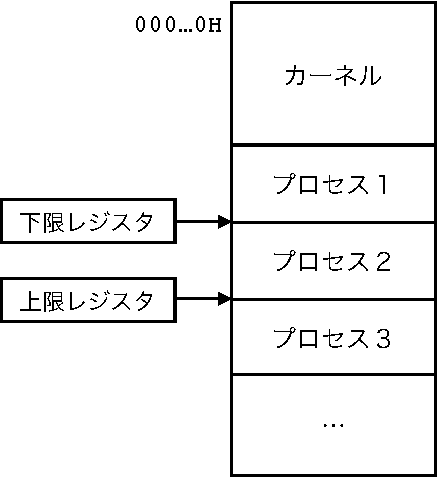
\includegraphics[scale=0.6]{Fig/baseLimitAddrSpace-crop.pdf}
      \subcaption{物理アドレス空間}
      \label{fig:baseLimitAddrSpace}
    \end{center}
  \end{minipage}
  \begin{minipage}{0.49\columnwidth}
    \begin{center}
      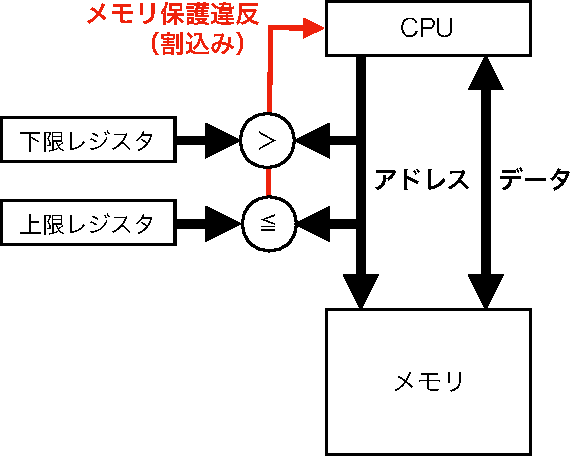
\includegraphics[scale=0.6]{Fig/baseLimitHardware-crop.pdf}
      \subcaption{ハードウェア構成}
      \label{fig:baseLimitHardware}
    \end{center}
  \end{minipage}
\end{myfig}

\begin{enumerate}
\item OSカーネルはプロセスの実行を開始する前に,
  プロセスの上限ドレスと下限ドレスを上限・下限レジスタに設定する.
  上限・下限レジスタを操作できるのはカーネルモード\footnote{
    実行モードは\ref{gen2nd}で紹介したので忘れた人は再確認すること.}で
  実行されるカーネルだけである.
  ユーザプロセスが自身のアクセスできる領域を変更することはできない.
\item カーネルはプロセスの実行を開始させる.
\item プロセスはユーザモードで実行される.
  ユーザモードで実行中は
  ハードウェアがCPUの出力するアドレスを上限・下限レジスタと比較する.
\item 上限・下限アドレスの範囲外へのアクセスの場合,
  ハードウェアがメモリアクセスを阻止しCPUに割込みをかける.
\item 割込みが発生するとユーザプロセスの実行が打ち切られ,
  制御がカーネルに移る.
\end{enumerate}

\subsection{ロック/キー機構}
主記憶をページに分割しページ毎にアクセス許可情報を持たせる.
64KiBのメモリを256ページに分割した例を\figref{lockKeyAddrSpace}に示す.
16bitのアドレスはページ番号を表す上位8bitと,
ページ内オフセットを表す下位8bitに分割される.

\figref{lockKeyHardware}に示すようにCPUは,
アドレス,アクセスキー,R/W/XをMMUに出力する.
アクセスキーはプロセス毎に決まる数字\footnote{プロセス番号でも良い.},
R/W/Xはメモリアクセスの種類を表す次のどれかである.
R(Read)は読み込みを,W(Write)書き込みを,
X(eXecute)は命令のフェッチを意味する.

MMUは許可情報表を内蔵している.
MMUはCPUが出力したアドレスからページ番号を求め表を引く.
表のプロテクションキーがアクセスキーと一致していない場合,
または,CPUのR/W/Xが表のアクセスモードに含まれていない場合は
メモリ保護違反の割込みを発生する.
MMUを操作できるのはCPUの実行モードがカーネルモードの時だけ,
MMUがメモリ保護違反の割込みを発生するのはユーザモード時だけである.

\begin{myfig}{btp}{ロック/キー機構の仕組み}{lockKey}
  \begin{minipage}{0.49\columnwidth}
    \begin{center}
      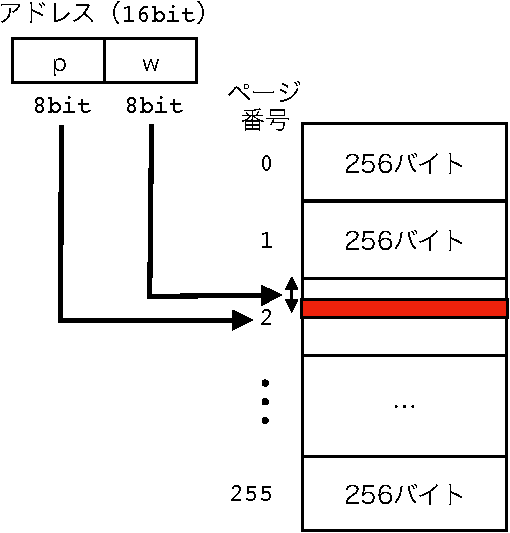
\includegraphics[scale=0.66]{Fig/lockKeyAddrSpace-crop.pdf}
      \subcaption{アドレス空間}
      \label{fig:lockKeyAddrSpace}
    \end{center}
  \end{minipage}
  \begin{minipage}{0.49\columnwidth}
    \begin{center}
      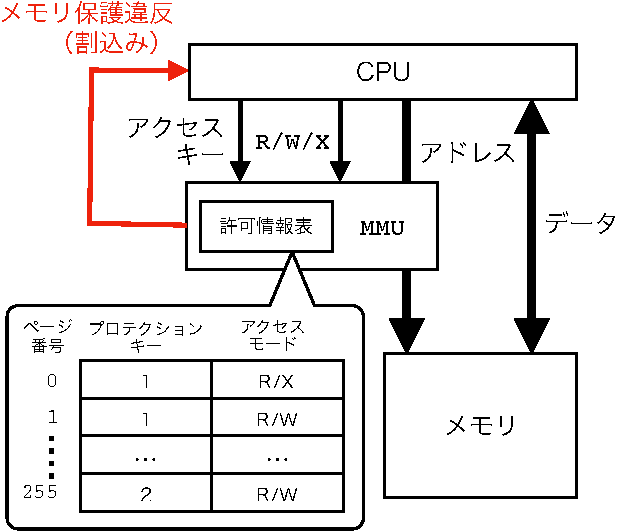
\includegraphics[scale=0.66]{Fig/lockKeyHardware-crop.pdf}
      \subcaption{ハードウェア構成}
      \label{fig:lockKeyHardware}
    \end{center}
  \end{minipage}
\end{myfig}

特別なプロテクションキー(例えば0)のページは
全てのプロセスがアクセス可能とすれば,
プロセス間の共有メモリを実現できる.

%==============================================================================
\section{プログラムの再配置}
コンパイルされたプログラムはメモリにロードされる時にアドレスが確定する.
ファイルに格納された実行可能形式プログラムは,
ロード時にアドレスを変更できる必要がある.

また,実行途中のプログラムのアドレスを変更することがある.
\figref{memoryCompaction}のようにメモリが多くの領域に分断され,
領域の間に小さなメモリの断片(\emph{メモリフラグメント})が沢山できた場合は,
プログラムの詰め合わせ(\emph{メモリコンパクション})を行う.
実行途中のプログラムを移動することを\emph{動的再配置}と呼ぶ.

\begin{myfig}{btp}{プログラムの動的再配置}{memoryCompaction}
  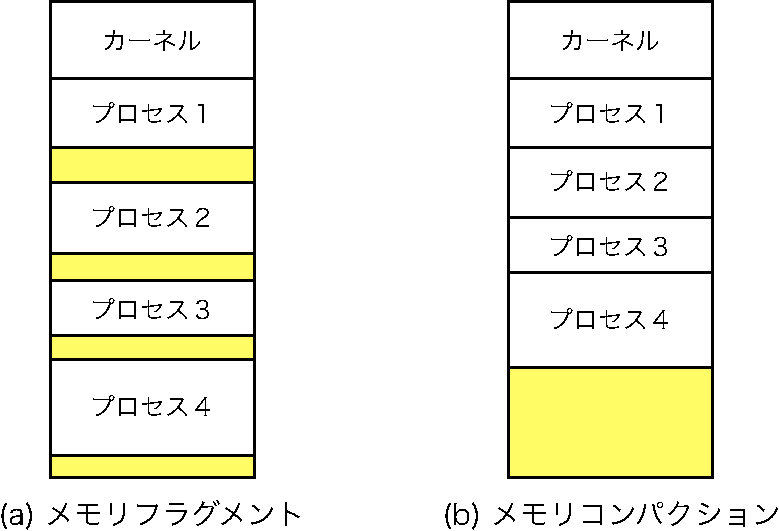
\includegraphics[scale=0.60]{Fig/memoryCompaction-crop.pdf}
\end{myfig}

\subsection{再配置可能オブジェクトファイル}
プログラミング言語で記述されたプログラムは,
コンパイルされ実行可能な機械語ファイルに変換される.
しかしコンパイル時には,
プログラムがメモリの何番地にロードされるか分からない.
そこで,
実行可能形式の機械語プログラムはジャンプ先アドレスや,
データアドレスの確定をロード時に行うことができなければならない.

ロードアドレスが確定しおらず,アドレスを変更可能な機械語プログラムは
\emph{再配置可能オブジェクト(relocatable object)}と呼ばれる.
再配置可能オブジェクトファイルは,
コンパイル済みの機械語プログラムの他に,
ファイル中のどの部分がアドレスであるかを記録した\emph{再配置表}も含む.
プログラムを主記憶にロードする際に再配置表を参照し,
プログラムやデータ中の全てのアドレス情報にロードアドレスを足し込む必要がある.
例えばプログラムを\|1234H|番地にロードすると,
\|JMP 0100H|の機械語は\|JMP 1334H|に書換える必要がある.
ロード時にアドレスを変換する方式を\emph{静的再配置}と呼ぶ.
再配置可能オブジェクトファイルの例としてTacOSが使用する
ファイルのフォーマットを付録\ref{appTacosFileFormat}に示す.

\subsection{リロケーションレジスタ}
動的再配置を行うためには,
実行中のプログラムがどこにアドレスを記憶しているか全て管理する必要がある.
しかし,CPUレジスタやスタックに書き込まれたアドレス,
リスト構造に含まれるポインタ等,
すべてのアドレスデータを追跡することは困難である.

動的再配置を可能にするための一つのアイデアは,
\emph{リロケーションレジスタ}と呼ばれる特別なハードウェアを用いることである.
\figref{relocationAddrSpace}に示すように\footnote{
  図はプロセス2を実行するための設定を表している}
リロケーションレジスタは,
プロセスのロードアドレス(B:Base)と大きさ(L:Limit)を記録するレジスタである.
ディスパッチャがプロセスを実行する時に値を設定する.

\figref{relocationHardware}に示すように
CPUが出力したアドレスはプロセスの大きさ(L)と比較される.
アドレスがL以上の場合はプロセス領域外のアドレスになるので
メモリ保護違反の割込みを発生する.
CPUのアドレスにプロセスのロードアドレス(B)を足した値がメモリアドレスになる.

\begin{myfig}{btp}{リロケーションレジスタ}{relocationRegister}
  \begin{minipage}{0.49\columnwidth}
    \begin{center}
      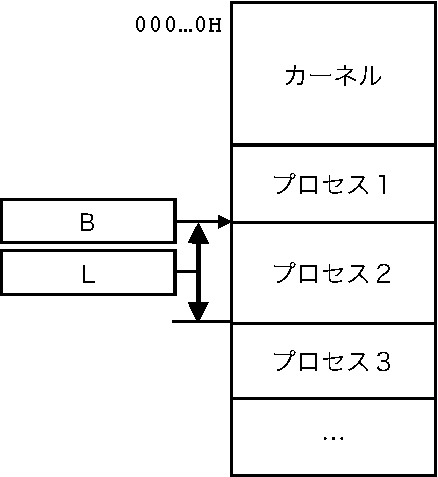
\includegraphics[scale=0.6]{Fig/relocationAddrSpace-crop.pdf}
      \subcaption{物理アドレス空間}
      \label{fig:relocationAddrSpace}
    \end{center}
  \end{minipage}
  \begin{minipage}{0.49\columnwidth}
    \begin{center}
      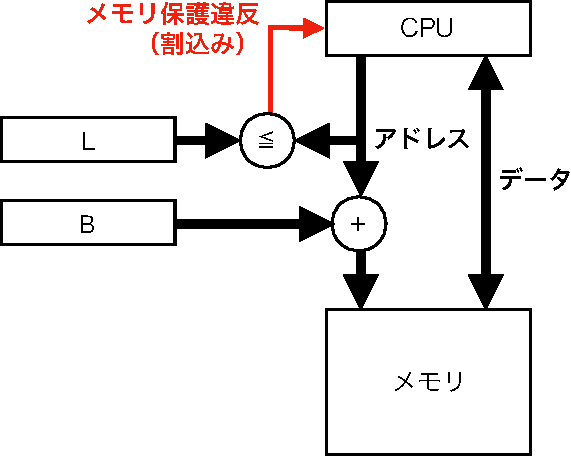
\includegraphics[scale=0.6]{Fig/relocationHardware-crop.pdf}
      \subcaption{ハードウェア構成}
      \label{fig:relocationHardware}
    \end{center}
  \end{minipage}
\end{myfig}

動的再配置を行うにはプロセスがRunning以外の状態の時に,
主記憶上でプロセスのメモリ領域を新しい領域にコピーする.
次回プロセスが実行される時,
ディスパッチャは新しい領域のアドレスをBにロードする.
ユーザプログラムは再配置されたことを知る必要はない.
しかし,プロセスの領域の移動は大量のメモリコピーを伴うので,
\emph{オーバーヘッドが大きい}処理である.

%==============================================================================
\section{アドレス空間の仮想化}
\figref{procOrganization}で示したように,
プロセスは各々が専用の\emph{仮想アドレス空間}(仮想メモリ空間)を持つ.
仮想アドレス空間は仮想アドレスで番地付けされている.
それに対しハードウェアとしてのメモリはシステム全体で一つしかない.
ハードウェアメモリは物理アドレスで番地付けされており,
\emph{物理アドレス空間}を形成する.
\figref{memorySpaceMapping}にプロセスの仮想アドレス空間が,
物理アドレス空間にマッピングされる様子を示す.
マッピングは,MMUよる仮想アドレスから物理アドレスへの変換によってなされる.

\begin{myfig}{btp}{仮想アドレス空間から物理アドレス空間へのマッピング}
  {memorySpaceMapping}
  \includegraphics[scale=0.60]{Fig/memorySpaceMapping-crop.pdf}
\end{myfig}

\subsection{単一仮想記憶}
多重仮想記憶に移行する中間的な形式である.
プロセスの仮想アドレスと物理アドレスが同じ方式である.
メリットが少ないので通常は次に紹介する多重仮想記憶を用いる.

\subsection{多重仮想記憶}
アドレス空間が仮想化されることにより,
全てのプロセスが0番地から始まるアドレス空間を持つことが可能になる.
プロセス毎に完全に独立したアドレス空間を持つ方式を\emph{多重仮想記憶}と呼ぶ.
実行可能形式のプログラムは,いつも0番地にロードされ実行される.
%再配置可能なオブジェクトでなくても良い.

\subsection{仮想アドレス空間の配置}
仮想アドレス空間にプログラムや変数を配置する方法は
オペレーティングシステムの種類により一定ではない.
\figref{memoryMapVsClang}とリスト\ref{cmmSample}に
UNIX上でC言語プログラムが配置される様子を示す.

\begin{myfig}{btp}{仮想アドレス空間の配置例}{memoryMapVsClang}
  \includegraphics[scale=0.6]{Fig/memoryMapVsClang-crop.pdf}
\end{myfig}

\begin{itemize}
\item 初期化済みのグローバル変数\footnote{
  正確には初期化済みの静的な変数.
  関数内で\texttt{static}修飾した変数も含まれる.}は,
  初期化データ領域(\emph{dataセグメント})に配置される.
\item 初期化されないグローバル変数\footnote{
  正確には初期化されない静的な変数.
  関数内で\texttt{static}修飾した変数も含まれる.}は,
  非初期化データ領域(\emph{bssセグメント})に配置される.
\item \texttt{main()}関数は機械語に変換され,
  プログラム領域(\emph{textセグメント})に配置される.
\item 関数のローカル変数\footnote{
  正確には自動変数.
  関数内で\texttt{static}修飾した変数は含まれない.}は,
  関数の実行開始時に\emph{スタック}または\emph{CPUレジスタ}に割り付けられ,
  関数を終了する時に破棄される.
  同じスタックを関数呼出しのために CALL 機械語命令も使用する.
  スタックは,必要に応じて仮想アドレス空間を0番地側に伸びていく.
\item \|malloc()|関数等を用いて動的に領域を割り当てると
  \emph{ヒープ}が使用される.
  ヒープは必要に応じて仮想アドレス空間を0番地とは逆の方向に伸びていく.
\end{itemize}

\lstinputlisting[caption=C言語プログラムをTaCの機械語に変換した例,
  numbers=none,float=btp,label=cmmSample]{Lst/cmmSample.s}
 % 主記憶
\begin{thebibliography}{9}

\bibitem{tec}
重村哲至,古川達也,相知政司,林 敏浩:
コンソールパネルを持つ機械語教育用マイコンの開発と授業への応用,
情報処理学会論文誌,Vol.48,No.9,pp.3318--3327(2007).

\bibitem{os360}
ウキペディア,
OS/360,
\url{https://ja.wikipedia.org/wiki/OS/360}(2017.10.03 閲覧)

\bibitem{mvs}
ウキペディア,
MVS,
\url{https://ja.wikipedia.org/wiki/Multiple_Virtual_Storage}(2017.10.03 閲覧)

\bibitem{os390}
ウキペディア,
OS/390,
\url{https://ja.wikipedia.org/wiki/OS/390}(2017.10.03 閲覧)

\bibitem{zos}
ウキペディア,
z/OS,
\url{https://ja.wikipedia.org/wiki/Z/OS}(2017.10.03 閲覧)

\bibitem{unix}
ウキペディア,
UNIX(「UNIXおよびUNIX系システムの系統図」を含む),
\url{https://ja.wikipedia.org/wiki/UNIX}(2017.10.03 閲覧)

\bibitem{solaris}
ウキペディア,
Solaris,
\url{https://ja.wikipedia.org/wiki/Solaris}(2017.10.03 閲覧)

\bibitem{aix}
ウキペディア,
AIX,
\url{https://ja.wikipedia.org/wiki/AIX}(2017.10.03 閲覧)

\bibitem{mach}
ウキペディア,
Mach,
\url{https://ja.wikipedia.org/wiki/Mach}(2017.10.03 閲覧)

\bibitem{bsdd}
ウキペディア,
BSDの子孫,
\url{https://ja.wikipedia.org/wiki/BSD%E3%81%AE%E5%AD%90%E5%AD%AB}(2017.10.03 閲覧)

\bibitem{bsd}
ウキペディア,
BSD,
\url{https://ja.wikipedia.org/wiki/BSD}(2017.10.04 閲覧)

\bibitem{386bsd}
ウキペディア,
386BSD,
\url{https://ja.wikipedia.org/wiki/386BSD}(2017.10.04 閲覧)

\bibitem{freebsd}
ウキペディア,
FreeBSD,
\url{https://ja.wikipedia.org/wiki/FreeBSD}(2017.10.03 閲覧)

\bibitem{freenas}
ウキペディア,
FreeNAS,
\url{https://ja.wikipedia.org/wiki/FreeNAS}(2017.10.03 閲覧)

\bibitem{nextstep}
ウキペディア,
NEXTSTEP,
\url{https://ja.wikipedia.org/wiki/NEXTSTEP}(2017.10.03 閲覧)

\bibitem{classicmacos}
ウキペディア,
Classic Mac OS,
\url{https://ja.wikipedia.org/wiki/Classic_Mac_OS}(2017.10.03 閲覧)

\bibitem{dynabook}
ウキペディア,
ダイナブック,
\url{
https://ja.wikipedia.org/wiki/ダイナブック
}(2017.10.03 閲覧)

\bibitem{macos}
ウキペディア,
macOS,
\url{
https://ja.wikipedia.org/wiki/MacOS
}(2017.10.03 閲覧)

\bibitem{ios}
ウキペディア,
iOS (アップル),
\url{
https://ja.wikipedia.org/wiki/IOS_(アップル)
}(2017.10.03 閲覧)

\bibitem{linux}
ウキペディア,
Linux,
\url{
https://ja.wikipedia.org/wiki/Linux
}(2017.10.03 閲覧)

\bibitem{android}
ウキペディア,
Andriod,
\url{
https://ja.wikipedia.org/wiki/Android
}(2017.10.03 閲覧)

\bibitem{msdos}
ウキペディア,
MS-DOS,
\url{
https://ja.wikipedia.org/wiki/MS-DOS
}(2017.10.03 閲覧)

\bibitem{windows}
ウキペディア,
Microsoft Windows(「Windows ファミリー系統図」含む),
\url{
https://ja.wikipedia.org/wiki/Microsoft_Windows
}(2017.10.03 閲覧)

\bibitem{ibmpc81}
ウキペディア,IBM PC,
\url{
https://ja.wikipedia.org/wiki/IBM_PC
}(2017.10.04 閲覧)

\bibitem{svr4}
ウキペディア,UNIX System V,
\url{
https://ja.wikipedia.org/wiki/UNIX_System_V
}(2017.10.04 閲覧)

\bibitem{iebsd}
重村哲至,情報電子工学科電算機室におけるPC-UNIXの歴史,
\url{
http://www2.tokuyama.ac.jp/giga/Sigemura/Public/IeNet/history.html
}(2017.10.03 閲覧)

\bibitem{linux1}
Linux kernel release 1.0,
\url{
https://www.kernel.org/pub/linux/kernel/v1.0/linux-1.0.tar.gz
}(2017.10.04)

\bibitem{third}
Andrew S. Tanenbaum, Herbert Bos:
``The Third Generaton(1965--1980):ICs and Multiproguramming'',
Modern Operating Systems(4th Edition),pp.9-14,
Pearson Education,Inc(2014).

\bibitem{fourth}
Andrew S. Tanenbaum, Herbert Bos:
``The Fourth Generation(1980--Present):Personal Computers'',
Modern Operating Systems(4th Edition),pp.15--19,
Pearson Education,Inc(2014).

\bibitem{key72}
Alan C. Kay:
``A Personal Computer for Children of All Ages'',
Proceeding ACM '72 Proceedings of the ACM annual conference - Volume 1
Article No 1 (1972).

\bibitem{key72J}
アラン・ケイ:すべての年齢の「子供たち」のためのパーソナルコンピュータ,
阿部和広,小学生からはじめるわくわくプログラミング,pp.130--141,
日経BP社(2013).

\bibitem{dynabook2}
アラン・ケイ:Dynabookとは何か?
「すべての年齢の「子供たち」のためのパーソナルコンピュータ」の後日談,
阿部和広,小学生からはじめるわくわくプログラミング,pp.142--149,
日経BP社(2013).

\bibitem{kei}
師尾 潤 他:スーパーコンピュータ「京」のオペレーティングシステム,
\url{http://img.jp.fujitsu.com/downloads/jp/jmag/vol63-3/paper07.pdf}
(2017.10.03 閲覧),
富士通(2012).

\bibitem{zfs}
Marshall Kirk McKusick,
George V. Neville-Neil,
Robert N. M. Watson:``The Zettabyte Filesystem,''
The Design and Implementation of the FreeBSD Operating System
Second Edition,Pearson Education,Inc,pp.523-550(2015).

%\bibitem{cpmJ}
%アンドリュー・S・タネンバウム,
%モダンオペレーティングシステム原著第2版,13ページ,
%ピアソン・エデュケーション(2004).

\bibitem{lines}
Andrew S. Tanenbaum, Herbert Bos:
``INTRODUCTION'',
Modern Operating Systems(4th Edition),pp.1-3,
Pearson Education,Inc(2014).

\bibitem{virtualization}
Andrew S. Tanenbaum, Herbert Bos:
``VIRTUALIZATION AND THE CLOUD'',
Modern Operating Systems(4th Edition),pp.471-516,
Pearson Education,Inc(2014).

\bibitem{vsphere}
ヴイエムウェア株式会社:
``VMware 徹底入門 第3版'',
廣済堂(2012).

\bibitem{ubuntu}
仮想ハードディスクイメージのダウンロード,
\url{https://www.ubuntulinux.jp/download/ja-remix-vhd}
(2017.10.19 閲覧),
Ubuntu Japanese Team(2012).

\bibitem{lightWeight}
Andrew S. Tanenbaum, Herbert Bos:
``Thread Usage'',
Modern Operating Systems(4th Edition),pp.97-102,
Pearson Education,Inc(2014).

\bibitem{hyperThreading}
ウキペディア,ハイパースレッディング・テクノロジー,
\url{
https://ja.wikipedia.org/wiki/%E3%83%8F%E3%82%A4%E3%83%91%E3%83%BC%E3%82%B9%E3%83%AC%E3%83%83%E3%83%87%E3%82%A3%E3%83%B3%E3%82%B0%E3%83%BB%E3%83%86%E3%82%AF%E3%83%8E%E3%83%AD%E3%82%B8%E3%83%BC
}(2017.11.02 閲覧)

\bibitem{AbstractDataType}
B.H.Liskov, S.N.Zilles:``Programming with Abstract Data Type'',
SIGPLAN Notices,9,4,pp.50-59(1974).

\bibitem{MemoryAllocation}
Abraham Silberschatz, Peter Baer Galvin, Greg Gagne:
``Memory Allocation'',
Operating System Concepts(9th Edition), pp.362-363,
John Wiley \& Sons,Inc(2013).

\bibitem{ia32Segmentation}
John H. Crawford, Patrick P. Gelsinger:``ベースとリミット'',
80386プログラミング, 工学社, pp.413-414(1988).

\bibitem{ia32SegmentReg}
John H. Crawford, Patrick P. Gelsinger:
``セグメント部:セグメント・レジスタ'',
80386プログラミング, 工学社, pp.48-50(1988).

\bibitem{ia32SegmentHiddenReg}
John H. Crawford, Patrick P. Gelsinger:
``デスクリプタ用の裏レジスタ'',
80386プログラミング, 工学社, pp.420-421(1988).

\bibitem{invertedPageTable}
Albert Chang, Mark F. Mergen:
``801 storage: architecture and programming'',
ACM Transactions on Computer Systems, 6, 1,
pp.28-50 (1988).

\bibitem{execOfFreeBSD}
Marshall Kirk McKusick,
George V. Neville-Neil,
Robert N. M. Watson:``Execution of a File'',
The Design and Implementation of the FreeBSD Operating System
Second Edition,Pearson Education,Inc,pp.262-263(2015).

\bibitem{wsClock}
Andrew S. Tanenbaum, Herbert Bos:
``The WSClock Page Replacement Algorithm'',
Modern Operating Systems(4th Edition),pp.219-221,
Pearson Education,Inc(2014).

\bibitem{RaidzOfFreeBSD}
Marshall Kirk McKusick,
George V. Neville-Neil,
Robert N. M. Watson:``RAIDZ'',
The Design and Implementation of the FreeBSD Operating System
Second Edition,Pearson Education,Inc,pp.540-541(2015).

\bibitem{DeduplicationOfFreeBSD}
Marshall Kirk McKusick,
George V. Neville-Neil,
Robert N. M. Watson:``Dedupliation'',
The Design and Implementation of the FreeBSD Operating System
Second Edition,Pearson Education,Inc,pp.545-546(2015).

\end{thebibliography}
 % 参考文献
\appendix
\chapter{TaCに関する資料}
\label{appTac}

%==============================================================================
\section{CPUの概要}
TaCで使用できるデータの形式,
CPU内部のレジスタ構成,
機械語命令について説明する.

\subsection{データ形式}
\figref{tacData}にTaCが扱うことができるデータ形式を示す.
16ビットの整数データと,16ビットのアドレスデータの他に,
8ビットのデータを扱うことができる.
16ビットのデータはCPUの内部でもメモリやI/Oでも使用できる.
メモリやI/Oの16ビットデータにアクセスする場合は偶数番地を用いる.
8ビットデータはメモリとI/Oの読み書きだけに使用できる.
メモリやI/Oの8ビットデータにアクセスする場合は,
CPUレジスタの下位8ビットが使用される.

\begin{myfig}{btp}{データ形式}{tacData}
  \includegraphics[scale=0.7]{Tbl/TaC7a-instruction-p1-1-crop.pdf}
\end{myfig}

\subsection{CPUレジスタとPSW}
\figref{tacRegPsw}にCPU内部のレジスタなどを示す.
レジスタはどれも16ビット幅である.
CPUレジスタは,
汎用のG0からG11,
フレームポインタとして使用するFP,
カーネルモード用のスタックポインタSSP,
ユーザモード用のスタックポインタUSPからなる.
これらは全て計算用にもアドレス用にも使用できる.
FP,SSP,USPは,以下に説明する特別な意味も持っている.

FPはフレームポインタ相対アドレッシングモードで使用できる.
このアドレッシングモードを用いると,
スタックフレーム内のローカル変数や関数引数へ,
1ワードの機械語命令でアクセスできる.

SSPはカーネルモードでSPの位置にマップされスタックポインタとして使用される.
USPはユーザモードでSPの位置にマップされスタックポインタとして使用される.
USPは最後のレジスタとして常時マップされており,
カーネルモードでもUSPをアクセスすることができる.

PSWはPCとFLAGからなる.
PCはプログラムカウンタのことである.
FLAGには,計算結果で変化するV,C,S,Zと,
割込み許可E,カーネルモードPの各ビットがある.
割込みが発生するとPCとFLAGが順にカーネルスタックにPUSHされた後で,
割込みが禁止された上でカーネルモードに切り換わる
(Eビットが0,Pビットが1になる).

\begin{myfig}{btp}{CPU内部の記憶装置}{tacRegPsw}
  \includegraphics[scale=0.7]{Tbl/TaC7a-instruction-p1-3-crop.pdf}
\end{myfig}

\subsection{機械語命令}
\figref{tacInsTbl}にTaCの機械語命令の一覧表を示す.
IN,OUT,RETI,EI,DI,HALTはカーネルモードでしか使用できない特権命令である.
SVC命令はシステムコールを発行するためにSVC割込みを発生する.

ほとんどの転送命令と計算命令で8種類のアドレッシング・モードが使用できる.
Direct,Indexed,Immediateの
三つのアドレッシング・モードを使用する場合は2ワードの機械語命令になる.
他のアドレッシング・モードの場合は全て1ワード命令である.

Byte Register Indirect アドレッシング・モードだけが,
メモリの8ビットデータをアクセスする.
Byte Register Indirect アドレッシング・モードの
ST命令はCPUレジスタの下位8ビットがメモリに書き込まれる.
その他の命令ではメモリから読み出した8ビットデータの上位に
\|00h|を付加した16ビットデータに変換して使用する.

\begin{myfig}{btp}{命令表}{tacInsTbl}
  \includegraphics[scale=0.94]{Tbl/TaC7a-instruction-p2-crop.pdf}
\end{myfig}

%==============================================================================
\newpage
\section{メモリマップとI/Oマップ}
\figref{tacMap}にTaCのメモリマップとI/Oマップを示す.
メモリやI/Oは8ビット毎にアドレス付けされており,
8ビットデータ,16ビットデータのどちらも読み書きできる.
アドレッシング・モードによって,8ビットデータと16ビットデータの区別をする.
16ビットデータは偶数アドレスを指定してアクセスしなければならない.

\subsection{メモリ空間}
TaCのメモリ空間は\|0000h|から\|FFFFh|の64KiBである.
16ビットデータは偶数アドレスからの2バイトに配置され,
偶数アドレスを指定してアクセスする.
16ビットデータにアクセスするには,
Byte Register Indirect モード\emph{以外}のアドレッシング・モードを用いる.
8ビットデータにアクセスするには,
Byte Register Indirect モードを用いる.

メモリ空間の最初から56KiBは自由に使用できるメモリであり,
ここにTacOSのカーネルやユーザプロセスがロードされる.
\|E000h|から\|EFFFh|まではVRAMが配置されている.
VRAMにASCIIコードを書き込むと対応する文字がディスプレイに表示される.
VRAMのアドレスがディスプレイの表示位置に対応する.
\|F000h|から\|FFDFh|はIPL(ROM)が配置される.
IPLはマイクロSDカードからTacOSを読み出して起動する.
\|FFE0h|から\|FFFFh|は割込みベクタ領域である.
16種類の割込みに対応するハンドラの入口番地をTacOSがセットする.

\subsection{I/O空間}
TaCのI/O空間は\|00h|から\|FFh|の256Bである.
I/O空間のアドレス幅は8ビットだが,
IN,OUT命令ではI/Oアドレスが16ビットで表現される.
I/Oアドレスの上位8ビットは\|00h|になるようにする.
上位8ビットが\|00h|以外になった場合の動作は保証されない.

メモリ空間と同様に8ビットデータと16ビットデータの両方を読み書きできる.
8ビットデータと16ビットデータの区別は,
IN,OUT命令のアドレッシングモードにより行う.
I/Oの8ビットデータにアクセスするには,
Byte Register Indirect モードを用いる.

\begin{myfig}{btp}{メモリマップとI/Oマップ}{tacMap}
  \includegraphics[scale=0.8]{Tbl/TaC7a-instruction-p4-crop.pdf}
\end{myfig}
  % 付録A

%------------------------------------------------------------------------------
% 発行元
\backmatter
\pagestyle{empty}
\onecolumn
~
\vfill\vfill\vfill
\begin{center}
\fbox{\parbox{10cm}{ \vspace{0.3cm}
\large{\bf{オペレーティングシステム Ver. 0.0.0}} \\
\\
 発行年月 2017年10月 Ver.0.0.0 \\
 発  行 独立行政法人国立高等専門学校機構 \\
      徳山工業高等専門学校 \\
      情報電子工学科 重村哲至 \\
      〒745-8585 山口県周南市学園台 \\
      sigemura@tokuyama.ac.jp \\
}}
\end{center}
\vfill
\end{document}
